%
% Copyright (c) 2006 XenSource, Inc.
%
% Permission is granted to copy, distribute and/or modify this document under
% the terms of the GNU Free Documentation License, Version 1.2 or any later
% version published by the Free Software Foundation; with no Invariant
% Sections, no Front-Cover Texts and no Back-Cover Texts.  A copy of the
% license is included in the section entitled
% "GNU Free Documentation License" or the file fdl.tex.
%
% Authors: Ewan Mellor, Richard Sharp, Dave Scott, Jon Harrop.
%

\chapter{API Reference}
\label{api-reference}


\section{Classes}
The following classes are defined:

\begin{center}\begin{tabular}{|lp{10cm}|}
\hline
Name & Description \\
\hline
{\tt session} & A session \\
{\tt task} & A long-running asynchronous task \\
{\tt event} & Asynchronous event registration and handling \\
{\tt VM} & A virtual machine (or 'guest') \\
{\tt VM\_metrics} & The metrics associated with a VM \\
{\tt VM\_guest\_metrics} & The metrics reported by the guest (as opposed to inferred from outside) \\
{\tt host} & A physical host \\
{\tt host\_metrics} & The metrics associated with a host \\
{\tt host\_cpu} & A physical CPU \\
{\tt network} & A virtual network \\
{\tt VIF} & A virtual network interface \\
{\tt VIF\_metrics} & The metrics associated with a virtual network device \\
{\tt PIF} & A physical network interface (note separate VLANs are represented as several PIFs) \\
{\tt PIF\_metrics} & The metrics associated with a physical network interface \\
{\tt SR} & A storage repository \\
{\tt VDI} & A virtual disk image \\
{\tt VBD} & A virtual block device \\
{\tt VBD\_metrics} & The metrics associated with a virtual block device \\
{\tt PBD} & The physical block devices through which hosts access SRs \\
{\tt crashdump} & A VM crashdump \\
{\tt VTPM} & A virtual TPM device \\
{\tt console} & A console \\
{\tt user} & A user of the system \\
{\tt debug} & A basic class for testing \\
\hline
\end{tabular}\end{center}
\section{Relationships Between Classes}
Fields that are bound together are shown in the following table: 
\begin{center}\begin{tabular}{|ll|l|}
\hline
{\em object.field} & {\em object.field} & {\em relationship} \\

\hline
host.PBDs & PBD.host & many-to-one\\
SR.PBDs & PBD.SR & many-to-one\\
VDI.VBDs & VBD.VDI & many-to-one\\
VDI.crash\_dumps & crashdump.VDI & many-to-one\\
VBD.VM & VM.VBDs & one-to-many\\
crashdump.VM & VM.crash\_dumps & one-to-many\\
VIF.VM & VM.VIFs & one-to-many\\
VIF.network & network.VIFs & one-to-many\\
PIF.host & host.PIFs & one-to-many\\
PIF.network & network.PIFs & one-to-many\\
SR.VDIs & VDI.SR & many-to-one\\
VTPM.VM & VM.VTPMs & one-to-many\\
console.VM & VM.consoles & one-to-many\\
host.resident\_VMs & VM.resident\_on & many-to-one\\
host.host\_CPUs & host\_cpu.host & many-to-one\\
\hline
\end{tabular}\end{center}

The following represents bound fields (as specified above) diagramatically, using crows-foot notation to specify one-to-one, one-to-many or many-to-many
                   relationships:

\begin{center}\resizebox{0.8\textwidth}{!}{
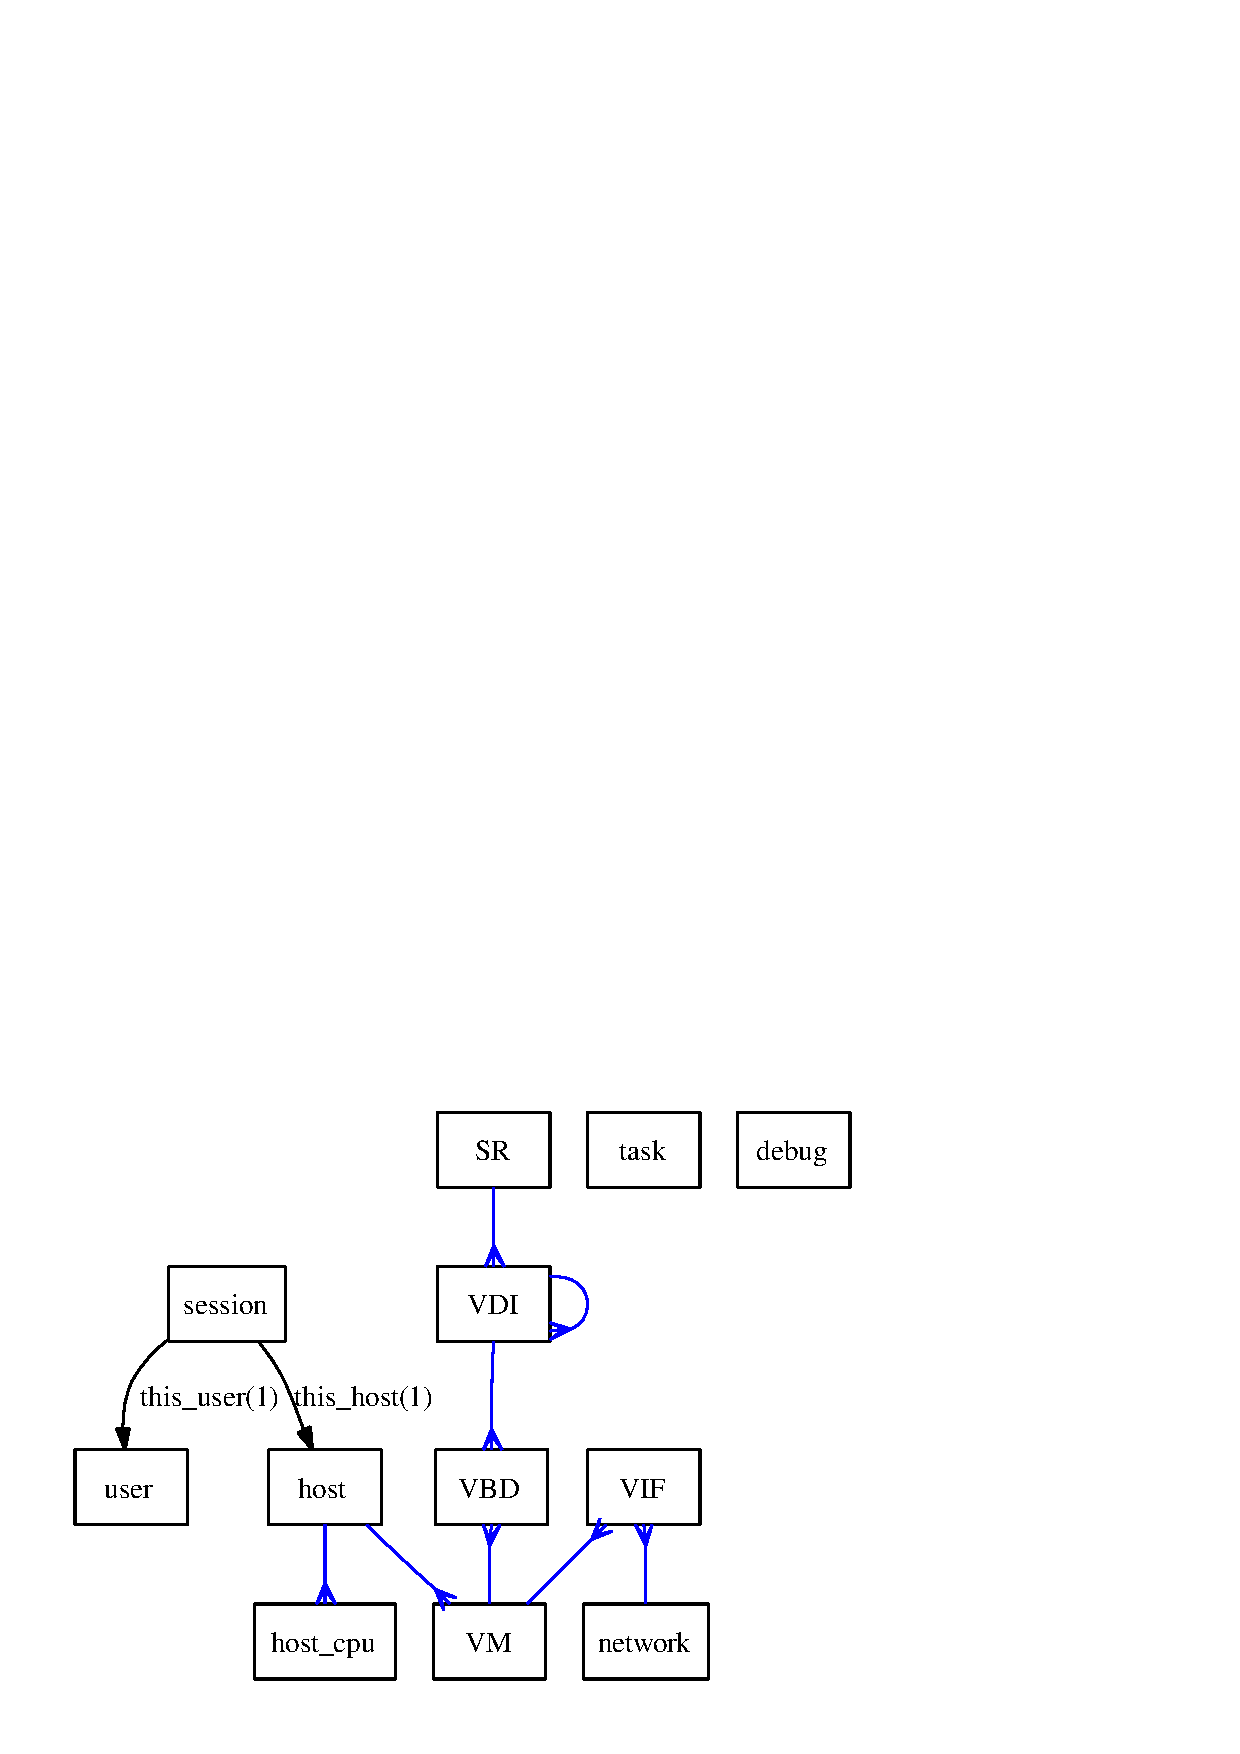
\includegraphics{xenapi-datamodel-graph}
}\end{center}
\
\subsection{List of bound fields}
\section{Types}
\subsection{Primitives}
The following primitive types are used to specify methods and fields in the API Reference:

\begin{center}\begin{tabular}{|ll|}
\hline
Type & Description \\
\hline
String & text strings \\
Int    & 64-bit integers \\
Float & IEEE double-precision floating-point numbers \\
Bool   & boolean \\
DateTime & date and timestamp \\
Ref (object name) & reference to an object of class name \\
\hline
\end{tabular}\end{center}
\subsection{Higher order types}
The following type constructors are used:

\begin{center}\begin{tabular}{|ll|}
\hline
Type & Description \\
\hline
List (t) & an arbitrary-length list of elements of type t \\
Map (a $\rightarrow$ b) & a table mapping values of type a to values of type b \\
\hline
\end{tabular}\end{center}
\subsection{Enumeration types}
The following enumeration types are used:

\begin{longtable}{|ll|}
\hline
{\tt enum event\_operation} & \\
\hline
\hspace{0.5cm}{\tt add} & An object has been created \\
\hspace{0.5cm}{\tt del} & An object has been deleted \\
\hspace{0.5cm}{\tt mod} & An object has been modified \\
\hline
\end{longtable}

\vspace{1cm}
\begin{longtable}{|ll|}
\hline
{\tt enum console\_protocol} & \\
\hline
\hspace{0.5cm}{\tt vt100} & VT100 terminal \\
\hspace{0.5cm}{\tt rfb} & Remote FrameBuffer protocol (as used in VNC) \\
\hspace{0.5cm}{\tt rdp} & Remote Desktop Protocol \\
\hline
\end{longtable}

\vspace{1cm}
\begin{longtable}{|ll|}
\hline
{\tt enum vdi\_type} & \\
\hline
\hspace{0.5cm}{\tt system} & a disk that may be replaced on upgrade \\
\hspace{0.5cm}{\tt user} & a disk that is always preserved on upgrade \\
\hspace{0.5cm}{\tt ephemeral} & a disk that may be reformatted on upgrade \\
\hspace{0.5cm}{\tt suspend} & a disk that stores a suspend image \\
\hspace{0.5cm}{\tt crashdump} & a disk that stores VM crashdump information \\
\hline
\end{longtable}

\vspace{1cm}
\begin{longtable}{|ll|}
\hline
{\tt enum vm\_power\_state} & \\
\hline
\hspace{0.5cm}{\tt Halted} & Halted \\
\hspace{0.5cm}{\tt Paused} & Paused \\
\hspace{0.5cm}{\tt Running} & Running \\
\hspace{0.5cm}{\tt Suspended} & Suspended \\
\hspace{0.5cm}{\tt Unknown} & Some other unknown state \\
\hline
\end{longtable}

\vspace{1cm}
\begin{longtable}{|ll|}
\hline
{\tt enum task\_allowed\_operations} & \\
\hline
\hspace{0.5cm}{\tt Cancel} & Cancel \\
\hline
\end{longtable}

\vspace{1cm}
\begin{longtable}{|ll|}
\hline
{\tt enum task\_status\_type} & \\
\hline
\hspace{0.5cm}{\tt pending} & task is in progress \\
\hspace{0.5cm}{\tt success} & task was completed successfully \\
\hspace{0.5cm}{\tt failure} & task has failed \\
\hspace{0.5cm}{\tt cancelling} & task is being cancelled \\
\hspace{0.5cm}{\tt cancelled} & task has been cancelled \\
\hline
\end{longtable}

\vspace{1cm}
\begin{longtable}{|ll|}
\hline
{\tt enum on\_normal\_exit} & \\
\hline
\hspace{0.5cm}{\tt destroy} & destroy the VM state \\
\hspace{0.5cm}{\tt restart} & restart the VM \\
\hline
\end{longtable}

\vspace{1cm}
\begin{longtable}{|ll|}
\hline
{\tt enum on\_crash\_behaviour} & \\
\hline
\hspace{0.5cm}{\tt destroy} & destroy the VM state \\
\hspace{0.5cm}{\tt coredump\_and\_destroy} & record a coredump and then destroy the VM state \\
\hspace{0.5cm}{\tt restart} & restart the VM \\
\hspace{0.5cm}{\tt coredump\_and\_restart} & record a coredump and then restart the VM \\
\hspace{0.5cm}{\tt preserve} & leave the crashed VM as-is \\
\hspace{0.5cm}{\tt rename\_restart} & rename the crashed VM and start a new copy \\
\hline
\end{longtable}

\vspace{1cm}
\begin{longtable}{|ll|}
\hline
{\tt enum vbd\_mode} & \\
\hline
\hspace{0.5cm}{\tt RO} & disk is mounted read-only \\
\hspace{0.5cm}{\tt RW} & disk is mounted read-write \\
\hline
\end{longtable}

\vspace{1cm}
\begin{longtable}{|ll|}
\hline
{\tt enum vbd\_type} & \\
\hline
\hspace{0.5cm}{\tt CD} & VBD will appear to guest as CD \\
\hspace{0.5cm}{\tt Disk} & VBD will appear to guest as disk \\
\hline
\end{longtable}

\vspace{1cm}

\newpage
\section{Class: session}
\subsection{Fields for class: session}
\begin{longtable}{|lllp{0.38\textwidth}|}
\hline
\multicolumn{1}{|l}{Name} & \multicolumn{3}{l|}{\bf session} \\
\multicolumn{1}{|l}{Description} & \multicolumn{3}{l|}{\parbox{11cm}{\em A
session.}} \\
\hline
Quals & Field & Type & Description \\
\hline
$\mathit{RO}_\mathit{run}$ &  {\tt uuid} & string & unique identifier/object reference \\
$\mathit{RO}_\mathit{run}$ &  {\tt this\_host} & host ref & Currently connected host \\
$\mathit{RO}_\mathit{run}$ &  {\tt this\_user} & user ref & Currently connected user \\
$\mathit{RO}_\mathit{run}$ &  {\tt last\_active} & int & Timestamp for last time session was active \\
\hline
\end{longtable}
\subsection{RPCs associated with class: session}
\subsubsection{RPC name:~login\_with\_password}

{\bf Overview:} 
Attempt to authenticate the user, returning a session\_id if successful.

 \noindent {\bf Signature:} 
\begin{verbatim} (session ref) login_with_password (string uname, string pwd)\end{verbatim}


\noindent{\bf Arguments:}

 
\vspace{0.3cm}
\begin{tabular}{|c|c|p{7cm}|}
 \hline
{\bf type} & {\bf name} & {\bf description} \\ \hline
{\tt string } & uname & Username for login. \\ \hline 

{\tt string } & pwd & Password for login. \\ \hline 

\end{tabular}

\vspace{0.3cm}

 \noindent {\bf Return Type:} 
{\tt 
session ref
}


ID of newly created session
\vspace{0.3cm}
\vspace{0.3cm}
\vspace{0.3cm}
\subsubsection{RPC name:~logout}

{\bf Overview:} 
Log out of a session.

 \noindent {\bf Signature:} 
\begin{verbatim} void logout (session_id s)\end{verbatim}


\vspace{0.3cm}

 \noindent {\bf Return Type:} 
{\tt 
void
}



\vspace{0.3cm}
\vspace{0.3cm}
\vspace{0.3cm}
\subsubsection{RPC name:~get\_uuid}

{\bf Overview:} 
Get the uuid field of the given session.

 \noindent {\bf Signature:} 
\begin{verbatim} string get_uuid (session_id s, session ref self)\end{verbatim}


\noindent{\bf Arguments:}

 
\vspace{0.3cm}
\begin{tabular}{|c|c|p{7cm}|}
 \hline
{\bf type} & {\bf name} & {\bf description} \\ \hline
{\tt session ref } & self & reference to the object \\ \hline 

\end{tabular}

\vspace{0.3cm}

 \noindent {\bf Return Type:} 
{\tt 
string
}


value of the field
\vspace{0.3cm}
\vspace{0.3cm}
\vspace{0.3cm}
\subsubsection{RPC name:~get\_this\_host}

{\bf Overview:} 
Get the this\_host field of the given session.

 \noindent {\bf Signature:} 
\begin{verbatim} (host ref) get_this_host (session_id s, session ref self)\end{verbatim}


\noindent{\bf Arguments:}

 
\vspace{0.3cm}
\begin{tabular}{|c|c|p{7cm}|}
 \hline
{\bf type} & {\bf name} & {\bf description} \\ \hline
{\tt session ref } & self & reference to the object \\ \hline 

\end{tabular}

\vspace{0.3cm}

 \noindent {\bf Return Type:} 
{\tt 
host ref
}


value of the field
\vspace{0.3cm}
\vspace{0.3cm}
\vspace{0.3cm}
\subsubsection{RPC name:~get\_this\_user}

{\bf Overview:} 
Get the this\_user field of the given session.

 \noindent {\bf Signature:} 
\begin{verbatim} (user ref) get_this_user (session_id s, session ref self)\end{verbatim}


\noindent{\bf Arguments:}

 
\vspace{0.3cm}
\begin{tabular}{|c|c|p{7cm}|}
 \hline
{\bf type} & {\bf name} & {\bf description} \\ \hline
{\tt session ref } & self & reference to the object \\ \hline 

\end{tabular}

\vspace{0.3cm}

 \noindent {\bf Return Type:} 
{\tt 
user ref
}


value of the field
\vspace{0.3cm}
\vspace{0.3cm}
\vspace{0.3cm}
\subsubsection{RPC name:~get\_last\_active}

{\bf Overview:} 
Get the last\_active field of the given session.

 \noindent {\bf Signature:} 
\begin{verbatim} int get_last_active (session_id s, session ref self)\end{verbatim}


\noindent{\bf Arguments:}

 
\vspace{0.3cm}
\begin{tabular}{|c|c|p{7cm}|}
 \hline
{\bf type} & {\bf name} & {\bf description} \\ \hline
{\tt session ref } & self & reference to the object \\ \hline 

\end{tabular}

\vspace{0.3cm}

 \noindent {\bf Return Type:} 
{\tt 
int
}


value of the field
\vspace{0.3cm}
\vspace{0.3cm}
\vspace{0.3cm}
\subsubsection{RPC name:~get\_by\_uuid}

{\bf Overview:} 
Get a reference to the session instance with the specified UUID.

 \noindent {\bf Signature:} 
\begin{verbatim} (session ref) get_by_uuid (session_id s, string uuid)\end{verbatim}


\noindent{\bf Arguments:}

 
\vspace{0.3cm}
\begin{tabular}{|c|c|p{7cm}|}
 \hline
{\bf type} & {\bf name} & {\bf description} \\ \hline
{\tt string } & uuid & UUID of object to return \\ \hline 

\end{tabular}

\vspace{0.3cm}

 \noindent {\bf Return Type:} 
{\tt 
session ref
}


reference to the object
\vspace{0.3cm}
\vspace{0.3cm}
\vspace{0.3cm}
\subsubsection{RPC name:~get\_record}

{\bf Overview:} 
Get a record containing the current state of the given session.

 \noindent {\bf Signature:} 
\begin{verbatim} (session record) get_record (session_id s, session ref self)\end{verbatim}


\noindent{\bf Arguments:}

 
\vspace{0.3cm}
\begin{tabular}{|c|c|p{7cm}|}
 \hline
{\bf type} & {\bf name} & {\bf description} \\ \hline
{\tt session ref } & self & reference to the object \\ \hline 

\end{tabular}

\vspace{0.3cm}

 \noindent {\bf Return Type:} 
{\tt 
session record
}


all fields from the object
\vspace{0.3cm}
\vspace{0.3cm}
\vspace{0.3cm}

\vspace{1cm}
\newpage
\section{Class: task}
\subsection{Fields for class: task}
\begin{longtable}{|lllp{0.38\textwidth}|}
\hline
\multicolumn{1}{|l}{Name} & \multicolumn{3}{l|}{\bf task} \\
\multicolumn{1}{|l}{Description} & \multicolumn{3}{l|}{\parbox{11cm}{\em A
long-running asynchronous task.}} \\
\hline
Quals & Field & Type & Description \\
\hline
$\mathit{RO}_\mathit{run}$ &  {\tt uuid} & string & unique identifier/object reference \\
$\mathit{RO}_\mathit{run}$ &  {\tt name/label} & string & a human-readable name \\
$\mathit{RO}_\mathit{run}$ &  {\tt name/description} & string & a notes field containg human-readable description \\
$\mathit{RO}_\mathit{run}$ &  {\tt status} & task\_status\_type & current status of the task \\
$\mathit{RO}_\mathit{run}$ &  {\tt session} & session ref & the session that created the task \\
$\mathit{RO}_\mathit{run}$ &  {\tt progress} & int & if the task is still pending, this field contains the estimated percentage complete (0-100). If task has completed (successfully or unsuccessfully) this should be 100. \\
$\mathit{RO}_\mathit{run}$ &  {\tt type} & string & if the task has completed successfully, this field contains the type of the encoded result (i.e. name of the class whose reference is in the result field). Undefined otherwise. \\
$\mathit{RO}_\mathit{run}$ &  {\tt result} & string & if the task has completed successfully, this field contains the result value (either Void or an object reference). Undefined otherwise. \\
$\mathit{RO}_\mathit{run}$ &  {\tt error\_code} & int & if the task has failed, this field contains the error code. Undefined otherwise. \\
$\mathit{RO}_\mathit{run}$ &  {\tt error\_info} & string Set & if the task has failed, this field contains the set of associated error strings. Undefined otherwise. \\
$\mathit{RO}_\mathit{run}$ &  {\tt allowed\_operations} & (task\_allowed\_operations) Set & Operations allowed on this task \\
\hline
\end{longtable}
\subsection{RPCs associated with class: task}
\subsubsection{RPC name:~cancel}

{\bf Overview:} 
Cancel this task.  If task.allowed\_operations does not contain Cancel,
then this will fail with OPERATION\_NOT\_ALLOWED.  The task will show the
status 'cancelling', and you should continue to check its status until it
shows 'cancelled'.  There is no guarantee as to the time within which this
task will be cancelled.

 \noindent {\bf Signature:} 
\begin{verbatim} void cancel (session_id s, task ref task)\end{verbatim}


\noindent{\bf Arguments:}

 
\vspace{0.3cm}
\begin{tabular}{|c|c|p{7cm}|}
 \hline
{\bf type} & {\bf name} & {\bf description} \\ \hline
{\tt task ref } & task & The task \\ \hline 

\end{tabular}

\vspace{0.3cm}

 \noindent {\bf Return Type:} 
{\tt 
void
}



\vspace{0.3cm}

\noindent{\bf Possible Error Codes:} {\tt OPERATION\_NOT\_ALLOWED}

\vspace{0.6cm}
\subsubsection{RPC name:~get\_all}

{\bf Overview:} 
Return a list of all the tasks known to the system.

 \noindent {\bf Signature:} 
\begin{verbatim} ((task ref) Set) get_all (session_id s)\end{verbatim}


\vspace{0.3cm}

 \noindent {\bf Return Type:} 
{\tt 
(task ref) Set
}


references to all objects
\vspace{0.3cm}
\vspace{0.3cm}
\vspace{0.3cm}
\subsubsection{RPC name:~get\_uuid}

{\bf Overview:} 
Get the uuid field of the given task.

 \noindent {\bf Signature:} 
\begin{verbatim} string get_uuid (session_id s, task ref self)\end{verbatim}


\noindent{\bf Arguments:}

 
\vspace{0.3cm}
\begin{tabular}{|c|c|p{7cm}|}
 \hline
{\bf type} & {\bf name} & {\bf description} \\ \hline
{\tt task ref } & self & reference to the object \\ \hline 

\end{tabular}

\vspace{0.3cm}

 \noindent {\bf Return Type:} 
{\tt 
string
}


value of the field
\vspace{0.3cm}
\vspace{0.3cm}
\vspace{0.3cm}
\subsubsection{RPC name:~get\_name\_label}

{\bf Overview:} 
Get the name/label field of the given task.

 \noindent {\bf Signature:} 
\begin{verbatim} string get_name_label (session_id s, task ref self)\end{verbatim}


\noindent{\bf Arguments:}

 
\vspace{0.3cm}
\begin{tabular}{|c|c|p{7cm}|}
 \hline
{\bf type} & {\bf name} & {\bf description} \\ \hline
{\tt task ref } & self & reference to the object \\ \hline 

\end{tabular}

\vspace{0.3cm}

 \noindent {\bf Return Type:} 
{\tt 
string
}


value of the field
\vspace{0.3cm}
\vspace{0.3cm}
\vspace{0.3cm}
\subsubsection{RPC name:~get\_name\_description}

{\bf Overview:} 
Get the name/description field of the given task.

 \noindent {\bf Signature:} 
\begin{verbatim} string get_name_description (session_id s, task ref self)\end{verbatim}


\noindent{\bf Arguments:}

 
\vspace{0.3cm}
\begin{tabular}{|c|c|p{7cm}|}
 \hline
{\bf type} & {\bf name} & {\bf description} \\ \hline
{\tt task ref } & self & reference to the object \\ \hline 

\end{tabular}

\vspace{0.3cm}

 \noindent {\bf Return Type:} 
{\tt 
string
}


value of the field
\vspace{0.3cm}
\vspace{0.3cm}
\vspace{0.3cm}
\subsubsection{RPC name:~get\_status}

{\bf Overview:} 
Get the status field of the given task.

 \noindent {\bf Signature:} 
\begin{verbatim} (task_status_type) get_status (session_id s, task ref self)\end{verbatim}


\noindent{\bf Arguments:}

 
\vspace{0.3cm}
\begin{tabular}{|c|c|p{7cm}|}
 \hline
{\bf type} & {\bf name} & {\bf description} \\ \hline
{\tt task ref } & self & reference to the object \\ \hline 

\end{tabular}

\vspace{0.3cm}

 \noindent {\bf Return Type:} 
{\tt 
task\_status\_type
}


value of the field
\vspace{0.3cm}
\vspace{0.3cm}
\vspace{0.3cm}
\subsubsection{RPC name:~get\_session}

{\bf Overview:} 
Get the session field of the given task.

 \noindent {\bf Signature:} 
\begin{verbatim} (session ref) get_session (session_id s, task ref self)\end{verbatim}


\noindent{\bf Arguments:}

 
\vspace{0.3cm}
\begin{tabular}{|c|c|p{7cm}|}
 \hline
{\bf type} & {\bf name} & {\bf description} \\ \hline
{\tt task ref } & self & reference to the object \\ \hline 

\end{tabular}

\vspace{0.3cm}

 \noindent {\bf Return Type:} 
{\tt 
session ref
}


value of the field
\vspace{0.3cm}
\vspace{0.3cm}
\vspace{0.3cm}
\subsubsection{RPC name:~get\_progress}

{\bf Overview:} 
Get the progress field of the given task.

 \noindent {\bf Signature:} 
\begin{verbatim} int get_progress (session_id s, task ref self)\end{verbatim}


\noindent{\bf Arguments:}

 
\vspace{0.3cm}
\begin{tabular}{|c|c|p{7cm}|}
 \hline
{\bf type} & {\bf name} & {\bf description} \\ \hline
{\tt task ref } & self & reference to the object \\ \hline 

\end{tabular}

\vspace{0.3cm}

 \noindent {\bf Return Type:} 
{\tt 
int
}


value of the field
\vspace{0.3cm}
\vspace{0.3cm}
\vspace{0.3cm}
\subsubsection{RPC name:~get\_type}

{\bf Overview:} 
Get the type field of the given task.

 \noindent {\bf Signature:} 
\begin{verbatim} string get_type (session_id s, task ref self)\end{verbatim}


\noindent{\bf Arguments:}

 
\vspace{0.3cm}
\begin{tabular}{|c|c|p{7cm}|}
 \hline
{\bf type} & {\bf name} & {\bf description} \\ \hline
{\tt task ref } & self & reference to the object \\ \hline 

\end{tabular}

\vspace{0.3cm}

 \noindent {\bf Return Type:} 
{\tt 
string
}


value of the field
\vspace{0.3cm}
\vspace{0.3cm}
\vspace{0.3cm}
\subsubsection{RPC name:~get\_result}

{\bf Overview:} 
Get the result field of the given task.

 \noindent {\bf Signature:} 
\begin{verbatim} string get_result (session_id s, task ref self)\end{verbatim}


\noindent{\bf Arguments:}

 
\vspace{0.3cm}
\begin{tabular}{|c|c|p{7cm}|}
 \hline
{\bf type} & {\bf name} & {\bf description} \\ \hline
{\tt task ref } & self & reference to the object \\ \hline 

\end{tabular}

\vspace{0.3cm}

 \noindent {\bf Return Type:} 
{\tt 
string
}


value of the field
\vspace{0.3cm}
\vspace{0.3cm}
\vspace{0.3cm}
\subsubsection{RPC name:~get\_error\_code}

{\bf Overview:} 
Get the error\_code field of the given task.

 \noindent {\bf Signature:} 
\begin{verbatim} int get_error_code (session_id s, task ref self)\end{verbatim}


\noindent{\bf Arguments:}

 
\vspace{0.3cm}
\begin{tabular}{|c|c|p{7cm}|}
 \hline
{\bf type} & {\bf name} & {\bf description} \\ \hline
{\tt task ref } & self & reference to the object \\ \hline 

\end{tabular}

\vspace{0.3cm}

 \noindent {\bf Return Type:} 
{\tt 
int
}


value of the field
\vspace{0.3cm}
\vspace{0.3cm}
\vspace{0.3cm}
\subsubsection{RPC name:~get\_error\_info}

{\bf Overview:} 
Get the error\_info field of the given task.

 \noindent {\bf Signature:} 
\begin{verbatim} (string Set) get_error_info (session_id s, task ref self)\end{verbatim}


\noindent{\bf Arguments:}

 
\vspace{0.3cm}
\begin{tabular}{|c|c|p{7cm}|}
 \hline
{\bf type} & {\bf name} & {\bf description} \\ \hline
{\tt task ref } & self & reference to the object \\ \hline 

\end{tabular}

\vspace{0.3cm}

 \noindent {\bf Return Type:} 
{\tt 
string Set
}


value of the field
\vspace{0.3cm}
\vspace{0.3cm}
\vspace{0.3cm}
\subsubsection{RPC name:~get\_allowed\_operations}

{\bf Overview:} 
Get the allowed\_operations field of the given task.

 \noindent {\bf Signature:} 
\begin{verbatim} ((task_allowed_operations) Set) get_allowed_operations (session_id s, task ref self)\end{verbatim}


\noindent{\bf Arguments:}

 
\vspace{0.3cm}
\begin{tabular}{|c|c|p{7cm}|}
 \hline
{\bf type} & {\bf name} & {\bf description} \\ \hline
{\tt task ref } & self & reference to the object \\ \hline 

\end{tabular}

\vspace{0.3cm}

 \noindent {\bf Return Type:} 
{\tt 
(task\_allowed\_operations) Set
}


value of the field
\vspace{0.3cm}
\vspace{0.3cm}
\vspace{0.3cm}
\subsubsection{RPC name:~get\_by\_uuid}

{\bf Overview:} 
Get a reference to the task instance with the specified UUID.

 \noindent {\bf Signature:} 
\begin{verbatim} (task ref) get_by_uuid (session_id s, string uuid)\end{verbatim}


\noindent{\bf Arguments:}

 
\vspace{0.3cm}
\begin{tabular}{|c|c|p{7cm}|}
 \hline
{\bf type} & {\bf name} & {\bf description} \\ \hline
{\tt string } & uuid & UUID of object to return \\ \hline 

\end{tabular}

\vspace{0.3cm}

 \noindent {\bf Return Type:} 
{\tt 
task ref
}


reference to the object
\vspace{0.3cm}
\vspace{0.3cm}
\vspace{0.3cm}
\subsubsection{RPC name:~get\_record}

{\bf Overview:} 
Get a record containing the current state of the given task.

 \noindent {\bf Signature:} 
\begin{verbatim} (task record) get_record (session_id s, task ref self)\end{verbatim}


\noindent{\bf Arguments:}

 
\vspace{0.3cm}
\begin{tabular}{|c|c|p{7cm}|}
 \hline
{\bf type} & {\bf name} & {\bf description} \\ \hline
{\tt task ref } & self & reference to the object \\ \hline 

\end{tabular}

\vspace{0.3cm}

 \noindent {\bf Return Type:} 
{\tt 
task record
}


all fields from the object
\vspace{0.3cm}
\vspace{0.3cm}
\vspace{0.3cm}
\subsubsection{RPC name:~get\_by\_name\_label}

{\bf Overview:} 
Get all the task instances with the given label.

 \noindent {\bf Signature:} 
\begin{verbatim} ((task ref) Set) get_by_name_label (session_id s, string label)\end{verbatim}


\noindent{\bf Arguments:}

 
\vspace{0.3cm}
\begin{tabular}{|c|c|p{7cm}|}
 \hline
{\bf type} & {\bf name} & {\bf description} \\ \hline
{\tt string } & label & label of object to return \\ \hline 

\end{tabular}

\vspace{0.3cm}

 \noindent {\bf Return Type:} 
{\tt 
(task ref) Set
}


references to objects with match names
\vspace{0.3cm}
\vspace{0.3cm}
\vspace{0.3cm}

\vspace{1cm}
\newpage
\section{Class: event}
\subsection{Fields for class: event}
\begin{longtable}{|lllp{0.38\textwidth}|}
\hline
\multicolumn{1}{|l}{Name} & \multicolumn{3}{l|}{\bf event} \\
\multicolumn{1}{|l}{Description} & \multicolumn{3}{l|}{\parbox{11cm}{\em
Asynchronous event registration and handling.}} \\
\hline
Quals & Field & Type & Description \\
\hline
$\mathit{RO}_\mathit{ins}$ &  {\tt id} & int & An ID, monotonically increasing, and local to the current session \\
$\mathit{RO}_\mathit{ins}$ &  {\tt timestamp} & datetime & The time at which the event occurred \\
$\mathit{RO}_\mathit{ins}$ &  {\tt class} & string & The name of the class of the object that changed \\
$\mathit{RO}_\mathit{ins}$ &  {\tt operation} & event\_operation & The operation that was performed \\
$\mathit{RO}_\mathit{ins}$ &  {\tt ref} & string & A reference to the object that changed \\
$\mathit{RO}_\mathit{ins}$ &  {\tt obj\_uuid} & string & The uuid of the object that changed \\
\hline
\end{longtable}
\subsection{RPCs associated with class: event}
\subsubsection{RPC name:~register}

{\bf Overview:} 
Registers this session with the event system.  Specifying the empty list
will register for all classes.

 \noindent {\bf Signature:} 
\begin{verbatim} void register (session_id s, string Set classes)\end{verbatim}


\noindent{\bf Arguments:}

 
\vspace{0.3cm}
\begin{tabular}{|c|c|p{7cm}|}
 \hline
{\bf type} & {\bf name} & {\bf description} \\ \hline
{\tt string Set } & classes & register for events for the indicated classes \\ \hline 

\end{tabular}

\vspace{0.3cm}

 \noindent {\bf Return Type:} 
{\tt 
void
}



\vspace{0.3cm}
\vspace{0.3cm}
\vspace{0.3cm}
\subsubsection{RPC name:~unregister}

{\bf Overview:} 
Unregisters this session with the event system.

 \noindent {\bf Signature:} 
\begin{verbatim} void unregister (session_id s, string Set classes)\end{verbatim}


\noindent{\bf Arguments:}

 
\vspace{0.3cm}
\begin{tabular}{|c|c|p{7cm}|}
 \hline
{\bf type} & {\bf name} & {\bf description} \\ \hline
{\tt string Set } & classes & remove this session's registration for the indicated classes \\ \hline 

\end{tabular}

\vspace{0.3cm}

 \noindent {\bf Return Type:} 
{\tt 
void
}



\vspace{0.3cm}
\vspace{0.3cm}
\vspace{0.3cm}
\subsubsection{RPC name:~next}

{\bf Overview:} 
Blocking call which returns a (possibly empty) batch of events.

 \noindent {\bf Signature:} 
\begin{verbatim} ((event record) Set) next (session_id s)\end{verbatim}


\vspace{0.3cm}

 \noindent {\bf Return Type:} 
{\tt 
(event record) Set
}


the batch of events
\vspace{0.3cm}
\vspace{0.3cm}
\vspace{0.3cm}

\vspace{1cm}
\newpage
\section{Class: VM}
\subsection{Fields for class: VM}
\begin{longtable}{|lllp{0.38\textwidth}|}
\hline
\multicolumn{1}{|l}{Name} & \multicolumn{3}{l|}{\bf VM} \\
\multicolumn{1}{|l}{Description} & \multicolumn{3}{l|}{\parbox{11cm}{\em A
virtual machine (or 'guest').}} \\
\hline
Quals & Field & Type & Description \\
\hline
$\mathit{RO}_\mathit{run}$ &  {\tt uuid} & string & unique identifier/object reference \\
$\mathit{RO}_\mathit{run}$ &  {\tt power\_state} & vm\_power\_state & Current power state of the machine \\
$\mathit{RW}$ &  {\tt name/label} & string & a human-readable name \\
$\mathit{RW}$ &  {\tt name/description} & string & a notes field containg human-readable description \\
$\mathit{RW}$ &  {\tt user\_version} & int & a user version number for this machine \\
$\mathit{RW}$ &  {\tt is\_a\_template} & bool & true if this is a template. Template VMs can never be started, they are used only for cloning other VMs \\
$\mathit{RW}$ &  {\tt auto\_power\_on} & bool & true if this VM should be started automatically after host boot \\
$\mathit{RO}_\mathit{run}$ &  {\tt suspend\_VDI} & VDI ref & The VDI that a suspend image is stored on. (Only has meaning if VM is currently suspended) \\
$\mathit{RO}_\mathit{run}$ &  {\tt resident\_on} & host ref & the host the VM is currently resident on \\
$\mathit{RW}$ &  {\tt memory/static\_max} & int & Statically-set (i.e. absolute) maximum (bytes) \\
$\mathit{RW}$ &  {\tt memory/dynamic\_max} & int & Dynamic maximum (bytes) \\
$\mathit{RW}$ &  {\tt memory/dynamic\_min} & int & Dynamic minimum (bytes) \\
$\mathit{RW}$ &  {\tt memory/static\_min} & int & Statically-set (i.e. absolute) mininum (bytes) \\
$\mathit{RW}$ &  {\tt VCPUs/params} & (string $\rightarrow$ string) Map & configuration parameters for the selected VCPU policy \\
$\mathit{RW}$ &  {\tt VCPUs/max} & int & Max number of VCPUs \\
$\mathit{RW}$ &  {\tt VCPUs/at\_startup} & int & Boot number of VCPUs \\
$\mathit{RW}$ &  {\tt actions/after\_shutdown} & on\_normal\_exit & action to take after the guest has shutdown itself \\
$\mathit{RW}$ &  {\tt actions/after\_reboot} & on\_normal\_exit & action to take after the guest has rebooted itself \\
$\mathit{RW}$ &  {\tt actions/after\_crash} & on\_crash\_behaviour & action to take if the guest crashes \\
$\mathit{RO}_\mathit{run}$ &  {\tt consoles} & (console ref) Set & virtual console devices \\
$\mathit{RO}_\mathit{run}$ &  {\tt VIFs} & (VIF ref) Set & virtual network interfaces \\
$\mathit{RO}_\mathit{run}$ &  {\tt VBDs} & (VBD ref) Set & virtual block devices \\
$\mathit{RO}_\mathit{run}$ &  {\tt crash\_dumps} & (crashdump ref) Set & crash dumps associated with this VM \\
$\mathit{RO}_\mathit{run}$ &  {\tt VTPMs} & (VTPM ref) Set & virtual TPMs \\
$\mathit{RW}$ &  {\tt PV/bootloader} & string & name of or path to bootloader \\
$\mathit{RW}$ &  {\tt PV/kernel} & string & path to the kernel \\
$\mathit{RW}$ &  {\tt PV/ramdisk} & string & path to the initrd \\
$\mathit{RW}$ &  {\tt PV/args} & string & kernel command-line arguments \\
$\mathit{RW}$ &  {\tt PV/bootloader\_args} & string & miscellaneous arguments for the bootloader \\
$\mathit{RW}$ &  {\tt HVM/boot\_policy} & string & HVM boot policy \\
$\mathit{RW}$ &  {\tt HVM/boot\_params} & (string $\rightarrow$ string) Map & HVM boot params \\
$\mathit{RW}$ &  {\tt platform} & (string $\rightarrow$ string) Map & platform-specific configuration \\
$\mathit{RW}$ &  {\tt PCI\_bus} & string & PCI bus path for pass-through devices \\
$\mathit{RW}$ &  {\tt other\_config} & (string $\rightarrow$ string) Map & additional configuration \\
$\mathit{RO}_\mathit{run}$ &  {\tt domid} & int & domain ID (if available, -1 otherwise) \\
$\mathit{RO}_\mathit{run}$ &  {\tt is\_control\_domain} & bool & true if this is a control domain (domain 0 or a driver domain) \\
$\mathit{RO}_\mathit{run}$ &  {\tt metrics} & VM\_metrics ref & metrics associated with this VM \\
$\mathit{RO}_\mathit{run}$ &  {\tt guest\_metrics} & VM\_guest\_metrics ref & metrics associated with the running guest \\
\hline
\end{longtable}
\subsection{RPCs associated with class: VM}
\subsubsection{RPC name:~clone}

{\bf Overview:} 
Clones the specified VM, making a new VM. Clone automatically exploits the
capabilities of the underlying storage repository in which the VM's disk
images are stored (e.g. Copy on Write).   This function can only be called
when the VM is in the Halted State.

 \noindent {\bf Signature:} 
\begin{verbatim} (VM ref) clone (session_id s, VM ref vm, string new_name)\end{verbatim}


\noindent{\bf Arguments:}

 
\vspace{0.3cm}
\begin{tabular}{|c|c|p{7cm}|}
 \hline
{\bf type} & {\bf name} & {\bf description} \\ \hline
{\tt VM ref } & vm & The VM to be cloned \\ \hline 

{\tt string } & new\_name & The name of the cloned VM \\ \hline 

\end{tabular}

\vspace{0.3cm}

 \noindent {\bf Return Type:} 
{\tt 
VM ref
}


The ID of the newly created VM.
\vspace{0.3cm}

\noindent{\bf Possible Error Codes:} {\tt VM\_BAD\_POWER\_STATE}

\vspace{0.6cm}
\subsubsection{RPC name:~start}

{\bf Overview:} 
Start the specified VM.  This function can only be called with the VM is in
the Halted State.

 \noindent {\bf Signature:} 
\begin{verbatim} void start (session_id s, VM ref vm, bool start_paused)\end{verbatim}


\noindent{\bf Arguments:}

 
\vspace{0.3cm}
\begin{tabular}{|c|c|p{7cm}|}
 \hline
{\bf type} & {\bf name} & {\bf description} \\ \hline
{\tt VM ref } & vm & The VM to start \\ \hline 

{\tt bool } & start\_paused & Instantiate VM in paused state if set to true. \\ \hline 

\end{tabular}

\vspace{0.3cm}

 \noindent {\bf Return Type:} 
{\tt 
void
}



\vspace{0.3cm}

\noindent{\bf Possible Error Codes:} {\tt VM\_BAD\_POWER\_STATE}, {\tt
VM\_HVM\_REQUIRED}

\vspace{0.6cm}
\subsubsection{RPC name:~pause}

{\bf Overview:} 
Pause the specified VM. This can only be called when the specified VM is in
the Running state.

 \noindent {\bf Signature:} 
\begin{verbatim} void pause (session_id s, VM ref vm)\end{verbatim}


\noindent{\bf Arguments:}

 
\vspace{0.3cm}
\begin{tabular}{|c|c|p{7cm}|}
 \hline
{\bf type} & {\bf name} & {\bf description} \\ \hline
{\tt VM ref } & vm & The VM to pause \\ \hline 

\end{tabular}

\vspace{0.3cm}

 \noindent {\bf Return Type:} 
{\tt 
void
}



\vspace{0.3cm}

\noindent{\bf Possible Error Codes:} {\tt VM\_BAD\_POWER\_STATE}

\vspace{0.6cm}
\subsubsection{RPC name:~unpause}

{\bf Overview:} 
Resume the specified VM. This can only be called when the specified VM is
in the Paused state.

 \noindent {\bf Signature:} 
\begin{verbatim} void unpause (session_id s, VM ref vm)\end{verbatim}


\noindent{\bf Arguments:}

 
\vspace{0.3cm}
\begin{tabular}{|c|c|p{7cm}|}
 \hline
{\bf type} & {\bf name} & {\bf description} \\ \hline
{\tt VM ref } & vm & The VM to unpause \\ \hline 

\end{tabular}

\vspace{0.3cm}

 \noindent {\bf Return Type:} 
{\tt 
void
}



\vspace{0.3cm}

\noindent{\bf Possible Error Codes:} {\tt VM\_BAD\_POWER\_STATE}

\vspace{0.6cm}
\subsubsection{RPC name:~clean\_shutdown}

{\bf Overview:} 
Attempt to cleanly shutdown the specified VM. (Note: this may not be
supported---e.g. if a guest agent is not installed).

Once shutdown has been completed perform poweroff action specified in guest
configuration.

This can only be called when the specified VM is in the Running state.

 \noindent {\bf Signature:} 
\begin{verbatim} void clean_shutdown (session_id s, VM ref vm)\end{verbatim}


\noindent{\bf Arguments:}

 
\vspace{0.3cm}
\begin{tabular}{|c|c|p{7cm}|}
 \hline
{\bf type} & {\bf name} & {\bf description} \\ \hline
{\tt VM ref } & vm & The VM to shutdown \\ \hline 

\end{tabular}

\vspace{0.3cm}

 \noindent {\bf Return Type:} 
{\tt 
void
}



\vspace{0.3cm}

\noindent{\bf Possible Error Codes:} {\tt VM\_BAD\_POWER\_STATE}

\vspace{0.6cm}
\subsubsection{RPC name:~clean\_reboot}

{\bf Overview:} 
Attempt to cleanly shutdown the specified VM (Note: this may not be
supported---e.g. if a guest agent is not installed).

Once shutdown has been completed perform reboot action specified in guest
configuration.

This can only be called when the specified VM is in the Running state.

 \noindent {\bf Signature:} 
\begin{verbatim} void clean_reboot (session_id s, VM ref vm)\end{verbatim}


\noindent{\bf Arguments:}

 
\vspace{0.3cm}
\begin{tabular}{|c|c|p{7cm}|}
 \hline
{\bf type} & {\bf name} & {\bf description} \\ \hline
{\tt VM ref } & vm & The VM to shutdown \\ \hline 

\end{tabular}

\vspace{0.3cm}

 \noindent {\bf Return Type:} 
{\tt 
void
}



\vspace{0.3cm}

\noindent{\bf Possible Error Codes:} {\tt VM\_BAD\_POWER\_STATE}

\vspace{0.6cm}
\subsubsection{RPC name:~hard\_shutdown}

{\bf Overview:} 
Stop executing the specified VM without attempting a clean shutdown. Then
perform poweroff action specified in VM configuration.

 \noindent {\bf Signature:} 
\begin{verbatim} void hard_shutdown (session_id s, VM ref vm)\end{verbatim}


\noindent{\bf Arguments:}

 
\vspace{0.3cm}
\begin{tabular}{|c|c|p{7cm}|}
 \hline
{\bf type} & {\bf name} & {\bf description} \\ \hline
{\tt VM ref } & vm & The VM to destroy \\ \hline 

\end{tabular}

\vspace{0.3cm}

 \noindent {\bf Return Type:} 
{\tt 
void
}



\vspace{0.3cm}

\noindent{\bf Possible Error Codes:} {\tt VM\_BAD\_POWER\_STATE}

\vspace{0.6cm}
\subsubsection{RPC name:~hard\_reboot}

{\bf Overview:} 
Stop executing the specified VM without attempting a clean shutdown. Then
perform reboot action specified in VM configuration.

 \noindent {\bf Signature:} 
\begin{verbatim} void hard_reboot (session_id s, VM ref vm)\end{verbatim}


\noindent{\bf Arguments:}

 
\vspace{0.3cm}
\begin{tabular}{|c|c|p{7cm}|}
 \hline
{\bf type} & {\bf name} & {\bf description} \\ \hline
{\tt VM ref } & vm & The VM to reboot \\ \hline 

\end{tabular}

\vspace{0.3cm}

 \noindent {\bf Return Type:} 
{\tt 
void
}



\vspace{0.3cm}
\vspace{0.3cm}
\vspace{0.3cm}
\subsubsection{RPC name:~suspend}

{\bf Overview:} 
Suspend the specified VM to disk.  This can only be called when the
specified VM is in the Running state.

 \noindent {\bf Signature:} 
\begin{verbatim} void suspend (session_id s, VM ref vm)\end{verbatim}


\noindent{\bf Arguments:}

 
\vspace{0.3cm}
\begin{tabular}{|c|c|p{7cm}|}
 \hline
{\bf type} & {\bf name} & {\bf description} \\ \hline
{\tt VM ref } & vm & The VM to suspend \\ \hline 

\end{tabular}

\vspace{0.3cm}

 \noindent {\bf Return Type:} 
{\tt 
void
}



\vspace{0.3cm}

\noindent{\bf Possible Error Codes:} {\tt VM\_BAD\_POWER\_STATE}

\vspace{0.6cm}
\subsubsection{RPC name:~resume}

{\bf Overview:} 
Awaken the specified VM and resume it.  This can only be called when the
specified VM is in the Suspended state.

 \noindent {\bf Signature:} 
\begin{verbatim} void resume (session_id s, VM ref vm, bool start_paused)\end{verbatim}


\noindent{\bf Arguments:}

 
\vspace{0.3cm}
\begin{tabular}{|c|c|p{7cm}|}
 \hline
{\bf type} & {\bf name} & {\bf description} \\ \hline
{\tt VM ref } & vm & The VM to resume \\ \hline 

{\tt bool } & start\_paused & Resume VM in paused state if set to true. \\ \hline 

\end{tabular}

\vspace{0.3cm}

 \noindent {\bf Return Type:} 
{\tt 
void
}



\vspace{0.3cm}

\noindent{\bf Possible Error Codes:} {\tt VM\_BAD\_POWER\_STATE}

\vspace{0.6cm}
\subsubsection{RPC name:~set\_VCPUs\_number\_live}

{\bf Overview:} 
Set this VM's VCPUs/at\_startup value, and set the same value on the VM, if
running.

 \noindent {\bf Signature:} 
\begin{verbatim} void set_VCPUs_number_live (session_id s, VM ref self, int nvcpu)\end{verbatim}


\noindent{\bf Arguments:}

 
\vspace{0.3cm}
\begin{tabular}{|c|c|p{7cm}|}
 \hline
{\bf type} & {\bf name} & {\bf description} \\ \hline
{\tt VM ref } & self & The VM \\ \hline 

{\tt int } & nvcpu & The number of VCPUs \\ \hline 

\end{tabular}

\vspace{0.3cm}

 \noindent {\bf Return Type:} 
{\tt 
void
}



\vspace{0.3cm}
\vspace{0.3cm}
\vspace{0.3cm}
\subsubsection{RPC name:~get\_all}

{\bf Overview:} 
Return a list of all the VMs known to the system.

 \noindent {\bf Signature:} 
\begin{verbatim} ((VM ref) Set) get_all (session_id s)\end{verbatim}


\vspace{0.3cm}

 \noindent {\bf Return Type:} 
{\tt 
(VM ref) Set
}


A list of all the IDs of all the VMs
\vspace{0.3cm}
\vspace{0.3cm}
\vspace{0.3cm}
\subsubsection{RPC name:~get\_uuid}

{\bf Overview:} 
Get the uuid field of the given VM.

 \noindent {\bf Signature:} 
\begin{verbatim} string get_uuid (session_id s, VM ref self)\end{verbatim}


\noindent{\bf Arguments:}

 
\vspace{0.3cm}
\begin{tabular}{|c|c|p{7cm}|}
 \hline
{\bf type} & {\bf name} & {\bf description} \\ \hline
{\tt VM ref } & self & reference to the object \\ \hline 

\end{tabular}

\vspace{0.3cm}

 \noindent {\bf Return Type:} 
{\tt 
string
}


value of the field
\vspace{0.3cm}
\vspace{0.3cm}
\vspace{0.3cm}
\subsubsection{RPC name:~get\_power\_state}

{\bf Overview:} 
Get the power\_state field of the given VM.

 \noindent {\bf Signature:} 
\begin{verbatim} (vm_power_state) get_power_state (session_id s, VM ref self)\end{verbatim}


\noindent{\bf Arguments:}

 
\vspace{0.3cm}
\begin{tabular}{|c|c|p{7cm}|}
 \hline
{\bf type} & {\bf name} & {\bf description} \\ \hline
{\tt VM ref } & self & reference to the object \\ \hline 

\end{tabular}

\vspace{0.3cm}

 \noindent {\bf Return Type:} 
{\tt 
vm\_power\_state
}


value of the field
\vspace{0.3cm}
\vspace{0.3cm}
\vspace{0.3cm}
\subsubsection{RPC name:~get\_name\_label}

{\bf Overview:} 
Get the name/label field of the given VM.

 \noindent {\bf Signature:} 
\begin{verbatim} string get_name_label (session_id s, VM ref self)\end{verbatim}


\noindent{\bf Arguments:}

 
\vspace{0.3cm}
\begin{tabular}{|c|c|p{7cm}|}
 \hline
{\bf type} & {\bf name} & {\bf description} \\ \hline
{\tt VM ref } & self & reference to the object \\ \hline 

\end{tabular}

\vspace{0.3cm}

 \noindent {\bf Return Type:} 
{\tt 
string
}


value of the field
\vspace{0.3cm}
\vspace{0.3cm}
\vspace{0.3cm}
\subsubsection{RPC name:~set\_name\_label}

{\bf Overview:} 
Set the name/label field of the given VM.

 \noindent {\bf Signature:} 
\begin{verbatim} void set_name_label (session_id s, VM ref self, string value)\end{verbatim}


\noindent{\bf Arguments:}

 
\vspace{0.3cm}
\begin{tabular}{|c|c|p{7cm}|}
 \hline
{\bf type} & {\bf name} & {\bf description} \\ \hline
{\tt VM ref } & self & reference to the object \\ \hline 

{\tt string } & value & New value to set \\ \hline 

\end{tabular}

\vspace{0.3cm}

 \noindent {\bf Return Type:} 
{\tt 
void
}



\vspace{0.3cm}
\vspace{0.3cm}
\vspace{0.3cm}
\subsubsection{RPC name:~get\_name\_description}

{\bf Overview:} 
Get the name/description field of the given VM.

 \noindent {\bf Signature:} 
\begin{verbatim} string get_name_description (session_id s, VM ref self)\end{verbatim}


\noindent{\bf Arguments:}

 
\vspace{0.3cm}
\begin{tabular}{|c|c|p{7cm}|}
 \hline
{\bf type} & {\bf name} & {\bf description} \\ \hline
{\tt VM ref } & self & reference to the object \\ \hline 

\end{tabular}

\vspace{0.3cm}

 \noindent {\bf Return Type:} 
{\tt 
string
}


value of the field
\vspace{0.3cm}
\vspace{0.3cm}
\vspace{0.3cm}
\subsubsection{RPC name:~set\_name\_description}

{\bf Overview:} 
Set the name/description field of the given VM.

 \noindent {\bf Signature:} 
\begin{verbatim} void set_name_description (session_id s, VM ref self, string value)\end{verbatim}


\noindent{\bf Arguments:}

 
\vspace{0.3cm}
\begin{tabular}{|c|c|p{7cm}|}
 \hline
{\bf type} & {\bf name} & {\bf description} \\ \hline
{\tt VM ref } & self & reference to the object \\ \hline 

{\tt string } & value & New value to set \\ \hline 

\end{tabular}

\vspace{0.3cm}

 \noindent {\bf Return Type:} 
{\tt 
void
}



\vspace{0.3cm}
\vspace{0.3cm}
\vspace{0.3cm}
\subsubsection{RPC name:~get\_user\_version}

{\bf Overview:} 
Get the user\_version field of the given VM.

 \noindent {\bf Signature:} 
\begin{verbatim} int get_user_version (session_id s, VM ref self)\end{verbatim}


\noindent{\bf Arguments:}

 
\vspace{0.3cm}
\begin{tabular}{|c|c|p{7cm}|}
 \hline
{\bf type} & {\bf name} & {\bf description} \\ \hline
{\tt VM ref } & self & reference to the object \\ \hline 

\end{tabular}

\vspace{0.3cm}

 \noindent {\bf Return Type:} 
{\tt 
int
}


value of the field
\vspace{0.3cm}
\vspace{0.3cm}
\vspace{0.3cm}
\subsubsection{RPC name:~set\_user\_version}

{\bf Overview:} 
Set the user\_version field of the given VM.

 \noindent {\bf Signature:} 
\begin{verbatim} void set_user_version (session_id s, VM ref self, int value)\end{verbatim}


\noindent{\bf Arguments:}

 
\vspace{0.3cm}
\begin{tabular}{|c|c|p{7cm}|}
 \hline
{\bf type} & {\bf name} & {\bf description} \\ \hline
{\tt VM ref } & self & reference to the object \\ \hline 

{\tt int } & value & New value to set \\ \hline 

\end{tabular}

\vspace{0.3cm}

 \noindent {\bf Return Type:} 
{\tt 
void
}



\vspace{0.3cm}
\vspace{0.3cm}
\vspace{0.3cm}
\subsubsection{RPC name:~get\_is\_a\_template}

{\bf Overview:} 
Get the is\_a\_template field of the given VM.

 \noindent {\bf Signature:} 
\begin{verbatim} bool get_is_a_template (session_id s, VM ref self)\end{verbatim}


\noindent{\bf Arguments:}

 
\vspace{0.3cm}
\begin{tabular}{|c|c|p{7cm}|}
 \hline
{\bf type} & {\bf name} & {\bf description} \\ \hline
{\tt VM ref } & self & reference to the object \\ \hline 

\end{tabular}

\vspace{0.3cm}

 \noindent {\bf Return Type:} 
{\tt 
bool
}


value of the field
\vspace{0.3cm}
\vspace{0.3cm}
\vspace{0.3cm}
\subsubsection{RPC name:~set\_is\_a\_template}

{\bf Overview:} 
Set the is\_a\_template field of the given VM.

 \noindent {\bf Signature:} 
\begin{verbatim} void set_is_a_template (session_id s, VM ref self, bool value)\end{verbatim}


\noindent{\bf Arguments:}

 
\vspace{0.3cm}
\begin{tabular}{|c|c|p{7cm}|}
 \hline
{\bf type} & {\bf name} & {\bf description} \\ \hline
{\tt VM ref } & self & reference to the object \\ \hline 

{\tt bool } & value & New value to set \\ \hline 

\end{tabular}

\vspace{0.3cm}

 \noindent {\bf Return Type:} 
{\tt 
void
}



\vspace{0.3cm}
\vspace{0.3cm}
\vspace{0.3cm}
\subsubsection{RPC name:~get\_auto\_power\_on}

{\bf Overview:} 
Get the auto\_power\_on field of the given VM.

 \noindent {\bf Signature:} 
\begin{verbatim} bool get_auto_power_on (session_id s, VM ref self)\end{verbatim}


\noindent{\bf Arguments:}

 
\vspace{0.3cm}
\begin{tabular}{|c|c|p{7cm}|}
 \hline
{\bf type} & {\bf name} & {\bf description} \\ \hline
{\tt VM ref } & self & reference to the object \\ \hline 

\end{tabular}

\vspace{0.3cm}

 \noindent {\bf Return Type:} 
{\tt 
bool
}


value of the field
\vspace{0.3cm}
\vspace{0.3cm}
\vspace{0.3cm}
\subsubsection{RPC name:~set\_auto\_power\_on}

{\bf Overview:} 
Set the auto\_power\_on field of the given VM.

 \noindent {\bf Signature:} 
\begin{verbatim} void set_auto_power_on (session_id s, VM ref self, bool value)\end{verbatim}


\noindent{\bf Arguments:}

 
\vspace{0.3cm}
\begin{tabular}{|c|c|p{7cm}|}
 \hline
{\bf type} & {\bf name} & {\bf description} \\ \hline
{\tt VM ref } & self & reference to the object \\ \hline 

{\tt bool } & value & New value to set \\ \hline 

\end{tabular}

\vspace{0.3cm}

 \noindent {\bf Return Type:} 
{\tt 
void
}



\vspace{0.3cm}
\vspace{0.3cm}
\vspace{0.3cm}
\subsubsection{RPC name:~get\_suspend\_VDI}

{\bf Overview:} 
Get the suspend\_VDI field of the given VM.

 \noindent {\bf Signature:} 
\begin{verbatim} (VDI ref) get_suspend_VDI (session_id s, VM ref self)\end{verbatim}


\noindent{\bf Arguments:}

 
\vspace{0.3cm}
\begin{tabular}{|c|c|p{7cm}|}
 \hline
{\bf type} & {\bf name} & {\bf description} \\ \hline
{\tt VM ref } & self & reference to the object \\ \hline 

\end{tabular}

\vspace{0.3cm}

 \noindent {\bf Return Type:} 
{\tt 
VDI ref
}


value of the field
\vspace{0.3cm}
\vspace{0.3cm}
\vspace{0.3cm}
\subsubsection{RPC name:~get\_resident\_on}

{\bf Overview:} 
Get the resident\_on field of the given VM.

 \noindent {\bf Signature:} 
\begin{verbatim} (host ref) get_resident_on (session_id s, VM ref self)\end{verbatim}


\noindent{\bf Arguments:}

 
\vspace{0.3cm}
\begin{tabular}{|c|c|p{7cm}|}
 \hline
{\bf type} & {\bf name} & {\bf description} \\ \hline
{\tt VM ref } & self & reference to the object \\ \hline 

\end{tabular}

\vspace{0.3cm}

 \noindent {\bf Return Type:} 
{\tt 
host ref
}


value of the field
\vspace{0.3cm}
\vspace{0.3cm}
\vspace{0.3cm}
\subsubsection{RPC name:~get\_memory\_static\_max}

{\bf Overview:} 
Get the memory/static\_max field of the given VM.

 \noindent {\bf Signature:} 
\begin{verbatim} int get_memory_static_max (session_id s, VM ref self)\end{verbatim}


\noindent{\bf Arguments:}

 
\vspace{0.3cm}
\begin{tabular}{|c|c|p{7cm}|}
 \hline
{\bf type} & {\bf name} & {\bf description} \\ \hline
{\tt VM ref } & self & reference to the object \\ \hline 

\end{tabular}

\vspace{0.3cm}

 \noindent {\bf Return Type:} 
{\tt 
int
}


value of the field
\vspace{0.3cm}
\vspace{0.3cm}
\vspace{0.3cm}
\subsubsection{RPC name:~set\_memory\_static\_max}

{\bf Overview:} 
Set the memory/static\_max field of the given VM.

 \noindent {\bf Signature:} 
\begin{verbatim} void set_memory_static_max (session_id s, VM ref self, int value)\end{verbatim}


\noindent{\bf Arguments:}

 
\vspace{0.3cm}
\begin{tabular}{|c|c|p{7cm}|}
 \hline
{\bf type} & {\bf name} & {\bf description} \\ \hline
{\tt VM ref } & self & reference to the object \\ \hline 

{\tt int } & value & New value to set \\ \hline 

\end{tabular}

\vspace{0.3cm}

 \noindent {\bf Return Type:} 
{\tt 
void
}



\vspace{0.3cm}
\vspace{0.3cm}
\vspace{0.3cm}
\subsubsection{RPC name:~get\_memory\_dynamic\_max}

{\bf Overview:} 
Get the memory/dynamic\_max field of the given VM.

 \noindent {\bf Signature:} 
\begin{verbatim} int get_memory_dynamic_max (session_id s, VM ref self)\end{verbatim}


\noindent{\bf Arguments:}

 
\vspace{0.3cm}
\begin{tabular}{|c|c|p{7cm}|}
 \hline
{\bf type} & {\bf name} & {\bf description} \\ \hline
{\tt VM ref } & self & reference to the object \\ \hline 

\end{tabular}

\vspace{0.3cm}

 \noindent {\bf Return Type:} 
{\tt 
int
}


value of the field
\vspace{0.3cm}
\vspace{0.3cm}
\vspace{0.3cm}
\subsubsection{RPC name:~set\_memory\_dynamic\_max}

{\bf Overview:} 
Set the memory/dynamic\_max field of the given VM.

 \noindent {\bf Signature:} 
\begin{verbatim} void set_memory_dynamic_max (session_id s, VM ref self, int value)\end{verbatim}


\noindent{\bf Arguments:}

 
\vspace{0.3cm}
\begin{tabular}{|c|c|p{7cm}|}
 \hline
{\bf type} & {\bf name} & {\bf description} \\ \hline
{\tt VM ref } & self & reference to the object \\ \hline 

{\tt int } & value & New value to set \\ \hline 

\end{tabular}

\vspace{0.3cm}

 \noindent {\bf Return Type:} 
{\tt 
void
}



\vspace{0.3cm}
\vspace{0.3cm}
\vspace{0.3cm}
\subsubsection{RPC name:~get\_memory\_dynamic\_min}

{\bf Overview:} 
Get the memory/dynamic\_min field of the given VM.

 \noindent {\bf Signature:} 
\begin{verbatim} int get_memory_dynamic_min (session_id s, VM ref self)\end{verbatim}


\noindent{\bf Arguments:}

 
\vspace{0.3cm}
\begin{tabular}{|c|c|p{7cm}|}
 \hline
{\bf type} & {\bf name} & {\bf description} \\ \hline
{\tt VM ref } & self & reference to the object \\ \hline 

\end{tabular}

\vspace{0.3cm}

 \noindent {\bf Return Type:} 
{\tt 
int
}


value of the field
\vspace{0.3cm}
\vspace{0.3cm}
\vspace{0.3cm}
\subsubsection{RPC name:~set\_memory\_dynamic\_min}

{\bf Overview:} 
Set the memory/dynamic\_min field of the given VM.

 \noindent {\bf Signature:} 
\begin{verbatim} void set_memory_dynamic_min (session_id s, VM ref self, int value)\end{verbatim}


\noindent{\bf Arguments:}

 
\vspace{0.3cm}
\begin{tabular}{|c|c|p{7cm}|}
 \hline
{\bf type} & {\bf name} & {\bf description} \\ \hline
{\tt VM ref } & self & reference to the object \\ \hline 

{\tt int } & value & New value to set \\ \hline 

\end{tabular}

\vspace{0.3cm}

 \noindent {\bf Return Type:} 
{\tt 
void
}



\vspace{0.3cm}
\vspace{0.3cm}
\vspace{0.3cm}
\subsubsection{RPC name:~get\_memory\_static\_min}

{\bf Overview:} 
Get the memory/static\_min field of the given VM.

 \noindent {\bf Signature:} 
\begin{verbatim} int get_memory_static_min (session_id s, VM ref self)\end{verbatim}


\noindent{\bf Arguments:}

 
\vspace{0.3cm}
\begin{tabular}{|c|c|p{7cm}|}
 \hline
{\bf type} & {\bf name} & {\bf description} \\ \hline
{\tt VM ref } & self & reference to the object \\ \hline 

\end{tabular}

\vspace{0.3cm}

 \noindent {\bf Return Type:} 
{\tt 
int
}


value of the field
\vspace{0.3cm}
\vspace{0.3cm}
\vspace{0.3cm}
\subsubsection{RPC name:~set\_memory\_static\_min}

{\bf Overview:} 
Set the memory/static\_min field of the given VM.

 \noindent {\bf Signature:} 
\begin{verbatim} void set_memory_static_min (session_id s, VM ref self, int value)\end{verbatim}


\noindent{\bf Arguments:}

 
\vspace{0.3cm}
\begin{tabular}{|c|c|p{7cm}|}
 \hline
{\bf type} & {\bf name} & {\bf description} \\ \hline
{\tt VM ref } & self & reference to the object \\ \hline 

{\tt int } & value & New value to set \\ \hline 

\end{tabular}

\vspace{0.3cm}

 \noindent {\bf Return Type:} 
{\tt 
void
}



\vspace{0.3cm}
\vspace{0.3cm}
\vspace{0.3cm}
\subsubsection{RPC name:~get\_VCPUs\_params}

{\bf Overview:} 
Get the VCPUs/params field of the given VM.

 \noindent {\bf Signature:} 
\begin{verbatim} ((string -> string) Map) get_VCPUs_params (session_id s, VM ref self)\end{verbatim}


\noindent{\bf Arguments:}

 
\vspace{0.3cm}
\begin{tabular}{|c|c|p{7cm}|}
 \hline
{\bf type} & {\bf name} & {\bf description} \\ \hline
{\tt VM ref } & self & reference to the object \\ \hline 

\end{tabular}

\vspace{0.3cm}

 \noindent {\bf Return Type:} 
{\tt 
(string $\rightarrow$ string) Map
}


value of the field
\vspace{0.3cm}
\vspace{0.3cm}
\vspace{0.3cm}
\subsubsection{RPC name:~set\_VCPUs\_params}

{\bf Overview:} 
Set the VCPUs/params field of the given VM.

 \noindent {\bf Signature:} 
\begin{verbatim} void set_VCPUs_params (session_id s, VM ref self, (string -> string) Map value)\end{verbatim}


\noindent{\bf Arguments:}

 
\vspace{0.3cm}
\begin{tabular}{|c|c|p{7cm}|}
 \hline
{\bf type} & {\bf name} & {\bf description} \\ \hline
{\tt VM ref } & self & reference to the object \\ \hline 

{\tt (string $\rightarrow$ string) Map } & value & New value to set \\ \hline 

\end{tabular}

\vspace{0.3cm}

 \noindent {\bf Return Type:} 
{\tt 
void
}



\vspace{0.3cm}
\vspace{0.3cm}
\vspace{0.3cm}
\subsubsection{RPC name:~add\_to\_VCPUs\_params}

{\bf Overview:} 
Add the given key-value pair to the VCPUs/params field of the given VM.

 \noindent {\bf Signature:} 
\begin{verbatim} void add_to_VCPUs_params (session_id s, VM ref self, string key, string value)\end{verbatim}


\noindent{\bf Arguments:}

 
\vspace{0.3cm}
\begin{tabular}{|c|c|p{7cm}|}
 \hline
{\bf type} & {\bf name} & {\bf description} \\ \hline
{\tt VM ref } & self & reference to the object \\ \hline 

{\tt string } & key & Key to add \\ \hline 

{\tt string } & value & Value to add \\ \hline 

\end{tabular}

\vspace{0.3cm}

 \noindent {\bf Return Type:} 
{\tt 
void
}



\vspace{0.3cm}
\vspace{0.3cm}
\vspace{0.3cm}
\subsubsection{RPC name:~remove\_from\_VCPUs\_params}

{\bf Overview:} 
Remove the given key and its corresponding value from the VCPUs/params
field of the given VM.  If the key is not in that Map, then do nothing.

 \noindent {\bf Signature:} 
\begin{verbatim} void remove_from_VCPUs_params (session_id s, VM ref self, string key)\end{verbatim}


\noindent{\bf Arguments:}

 
\vspace{0.3cm}
\begin{tabular}{|c|c|p{7cm}|}
 \hline
{\bf type} & {\bf name} & {\bf description} \\ \hline
{\tt VM ref } & self & reference to the object \\ \hline 

{\tt string } & key & Key to remove \\ \hline 

\end{tabular}

\vspace{0.3cm}

 \noindent {\bf Return Type:} 
{\tt 
void
}



\vspace{0.3cm}
\vspace{0.3cm}
\vspace{0.3cm}
\subsubsection{RPC name:~get\_VCPUs\_max}

{\bf Overview:} 
Get the VCPUs/max field of the given VM.

 \noindent {\bf Signature:} 
\begin{verbatim} int get_VCPUs_max (session_id s, VM ref self)\end{verbatim}


\noindent{\bf Arguments:}

 
\vspace{0.3cm}
\begin{tabular}{|c|c|p{7cm}|}
 \hline
{\bf type} & {\bf name} & {\bf description} \\ \hline
{\tt VM ref } & self & reference to the object \\ \hline 

\end{tabular}

\vspace{0.3cm}

 \noindent {\bf Return Type:} 
{\tt 
int
}


value of the field
\vspace{0.3cm}
\vspace{0.3cm}
\vspace{0.3cm}
\subsubsection{RPC name:~set\_VCPUs\_max}

{\bf Overview:} 
Set the VCPUs/max field of the given VM.

 \noindent {\bf Signature:} 
\begin{verbatim} void set_VCPUs_max (session_id s, VM ref self, int value)\end{verbatim}


\noindent{\bf Arguments:}

 
\vspace{0.3cm}
\begin{tabular}{|c|c|p{7cm}|}
 \hline
{\bf type} & {\bf name} & {\bf description} \\ \hline
{\tt VM ref } & self & reference to the object \\ \hline 

{\tt int } & value & New value to set \\ \hline 

\end{tabular}

\vspace{0.3cm}

 \noindent {\bf Return Type:} 
{\tt 
void
}



\vspace{0.3cm}
\vspace{0.3cm}
\vspace{0.3cm}
\subsubsection{RPC name:~get\_VCPUs\_at\_startup}

{\bf Overview:} 
Get the VCPUs/at\_startup field of the given VM.

 \noindent {\bf Signature:} 
\begin{verbatim} int get_VCPUs_at_startup (session_id s, VM ref self)\end{verbatim}


\noindent{\bf Arguments:}

 
\vspace{0.3cm}
\begin{tabular}{|c|c|p{7cm}|}
 \hline
{\bf type} & {\bf name} & {\bf description} \\ \hline
{\tt VM ref } & self & reference to the object \\ \hline 

\end{tabular}

\vspace{0.3cm}

 \noindent {\bf Return Type:} 
{\tt 
int
}


value of the field
\vspace{0.3cm}
\vspace{0.3cm}
\vspace{0.3cm}
\subsubsection{RPC name:~set\_VCPUs\_at\_startup}

{\bf Overview:} 
Set the VCPUs/at\_startup field of the given VM.

 \noindent {\bf Signature:} 
\begin{verbatim} void set_VCPUs_at_startup (session_id s, VM ref self, int value)\end{verbatim}


\noindent{\bf Arguments:}

 
\vspace{0.3cm}
\begin{tabular}{|c|c|p{7cm}|}
 \hline
{\bf type} & {\bf name} & {\bf description} \\ \hline
{\tt VM ref } & self & reference to the object \\ \hline 

{\tt int } & value & New value to set \\ \hline 

\end{tabular}

\vspace{0.3cm}

 \noindent {\bf Return Type:} 
{\tt 
void
}



\vspace{0.3cm}
\vspace{0.3cm}
\vspace{0.3cm}
\subsubsection{RPC name:~get\_actions\_after\_shutdown}

{\bf Overview:} 
Get the actions/after\_shutdown field of the given VM.

 \noindent {\bf Signature:} 
\begin{verbatim} (on_normal_exit) get_actions_after_shutdown (session_id s, VM ref self)\end{verbatim}


\noindent{\bf Arguments:}

 
\vspace{0.3cm}
\begin{tabular}{|c|c|p{7cm}|}
 \hline
{\bf type} & {\bf name} & {\bf description} \\ \hline
{\tt VM ref } & self & reference to the object \\ \hline 

\end{tabular}

\vspace{0.3cm}

 \noindent {\bf Return Type:} 
{\tt 
on\_normal\_exit
}


value of the field
\vspace{0.3cm}
\vspace{0.3cm}
\vspace{0.3cm}
\subsubsection{RPC name:~set\_actions\_after\_shutdown}

{\bf Overview:} 
Set the actions/after\_shutdown field of the given VM.

 \noindent {\bf Signature:} 
\begin{verbatim} void set_actions_after_shutdown (session_id s, VM ref self, on_normal_exit value)\end{verbatim}


\noindent{\bf Arguments:}

 
\vspace{0.3cm}
\begin{tabular}{|c|c|p{7cm}|}
 \hline
{\bf type} & {\bf name} & {\bf description} \\ \hline
{\tt VM ref } & self & reference to the object \\ \hline 

{\tt on\_normal\_exit } & value & New value to set \\ \hline 

\end{tabular}

\vspace{0.3cm}

 \noindent {\bf Return Type:} 
{\tt 
void
}



\vspace{0.3cm}
\vspace{0.3cm}
\vspace{0.3cm}
\subsubsection{RPC name:~get\_actions\_after\_reboot}

{\bf Overview:} 
Get the actions/after\_reboot field of the given VM.

 \noindent {\bf Signature:} 
\begin{verbatim} (on_normal_exit) get_actions_after_reboot (session_id s, VM ref self)\end{verbatim}


\noindent{\bf Arguments:}

 
\vspace{0.3cm}
\begin{tabular}{|c|c|p{7cm}|}
 \hline
{\bf type} & {\bf name} & {\bf description} \\ \hline
{\tt VM ref } & self & reference to the object \\ \hline 

\end{tabular}

\vspace{0.3cm}

 \noindent {\bf Return Type:} 
{\tt 
on\_normal\_exit
}


value of the field
\vspace{0.3cm}
\vspace{0.3cm}
\vspace{0.3cm}
\subsubsection{RPC name:~set\_actions\_after\_reboot}

{\bf Overview:} 
Set the actions/after\_reboot field of the given VM.

 \noindent {\bf Signature:} 
\begin{verbatim} void set_actions_after_reboot (session_id s, VM ref self, on_normal_exit value)\end{verbatim}


\noindent{\bf Arguments:}

 
\vspace{0.3cm}
\begin{tabular}{|c|c|p{7cm}|}
 \hline
{\bf type} & {\bf name} & {\bf description} \\ \hline
{\tt VM ref } & self & reference to the object \\ \hline 

{\tt on\_normal\_exit } & value & New value to set \\ \hline 

\end{tabular}

\vspace{0.3cm}

 \noindent {\bf Return Type:} 
{\tt 
void
}



\vspace{0.3cm}
\vspace{0.3cm}
\vspace{0.3cm}
\subsubsection{RPC name:~get\_actions\_after\_crash}

{\bf Overview:} 
Get the actions/after\_crash field of the given VM.

 \noindent {\bf Signature:} 
\begin{verbatim} (on_crash_behaviour) get_actions_after_crash (session_id s, VM ref self)\end{verbatim}


\noindent{\bf Arguments:}

 
\vspace{0.3cm}
\begin{tabular}{|c|c|p{7cm}|}
 \hline
{\bf type} & {\bf name} & {\bf description} \\ \hline
{\tt VM ref } & self & reference to the object \\ \hline 

\end{tabular}

\vspace{0.3cm}

 \noindent {\bf Return Type:} 
{\tt 
on\_crash\_behaviour
}


value of the field
\vspace{0.3cm}
\vspace{0.3cm}
\vspace{0.3cm}
\subsubsection{RPC name:~set\_actions\_after\_crash}

{\bf Overview:} 
Set the actions/after\_crash field of the given VM.

 \noindent {\bf Signature:} 
\begin{verbatim} void set_actions_after_crash (session_id s, VM ref self, on_crash_behaviour value)\end{verbatim}


\noindent{\bf Arguments:}

 
\vspace{0.3cm}
\begin{tabular}{|c|c|p{7cm}|}
 \hline
{\bf type} & {\bf name} & {\bf description} \\ \hline
{\tt VM ref } & self & reference to the object \\ \hline 

{\tt on\_crash\_behaviour } & value & New value to set \\ \hline 

\end{tabular}

\vspace{0.3cm}

 \noindent {\bf Return Type:} 
{\tt 
void
}



\vspace{0.3cm}
\vspace{0.3cm}
\vspace{0.3cm}
\subsubsection{RPC name:~get\_consoles}

{\bf Overview:} 
Get the consoles field of the given VM.

 \noindent {\bf Signature:} 
\begin{verbatim} ((console ref) Set) get_consoles (session_id s, VM ref self)\end{verbatim}


\noindent{\bf Arguments:}

 
\vspace{0.3cm}
\begin{tabular}{|c|c|p{7cm}|}
 \hline
{\bf type} & {\bf name} & {\bf description} \\ \hline
{\tt VM ref } & self & reference to the object \\ \hline 

\end{tabular}

\vspace{0.3cm}

 \noindent {\bf Return Type:} 
{\tt 
(console ref) Set
}


value of the field
\vspace{0.3cm}
\vspace{0.3cm}
\vspace{0.3cm}
\subsubsection{RPC name:~get\_VIFs}

{\bf Overview:} 
Get the VIFs field of the given VM.

 \noindent {\bf Signature:} 
\begin{verbatim} ((VIF ref) Set) get_VIFs (session_id s, VM ref self)\end{verbatim}


\noindent{\bf Arguments:}

 
\vspace{0.3cm}
\begin{tabular}{|c|c|p{7cm}|}
 \hline
{\bf type} & {\bf name} & {\bf description} \\ \hline
{\tt VM ref } & self & reference to the object \\ \hline 

\end{tabular}

\vspace{0.3cm}

 \noindent {\bf Return Type:} 
{\tt 
(VIF ref) Set
}


value of the field
\vspace{0.3cm}
\vspace{0.3cm}
\vspace{0.3cm}
\subsubsection{RPC name:~get\_VBDs}

{\bf Overview:} 
Get the VBDs field of the given VM.

 \noindent {\bf Signature:} 
\begin{verbatim} ((VBD ref) Set) get_VBDs (session_id s, VM ref self)\end{verbatim}


\noindent{\bf Arguments:}

 
\vspace{0.3cm}
\begin{tabular}{|c|c|p{7cm}|}
 \hline
{\bf type} & {\bf name} & {\bf description} \\ \hline
{\tt VM ref } & self & reference to the object \\ \hline 

\end{tabular}

\vspace{0.3cm}

 \noindent {\bf Return Type:} 
{\tt 
(VBD ref) Set
}


value of the field
\vspace{0.3cm}
\vspace{0.3cm}
\vspace{0.3cm}
\subsubsection{RPC name:~get\_crash\_dumps}

{\bf Overview:} 
Get the crash\_dumps field of the given VM.

 \noindent {\bf Signature:} 
\begin{verbatim} ((crashdump ref) Set) get_crash_dumps (session_id s, VM ref self)\end{verbatim}


\noindent{\bf Arguments:}

 
\vspace{0.3cm}
\begin{tabular}{|c|c|p{7cm}|}
 \hline
{\bf type} & {\bf name} & {\bf description} \\ \hline
{\tt VM ref } & self & reference to the object \\ \hline 

\end{tabular}

\vspace{0.3cm}

 \noindent {\bf Return Type:} 
{\tt 
(crashdump ref) Set
}


value of the field
\vspace{0.3cm}
\vspace{0.3cm}
\vspace{0.3cm}
\subsubsection{RPC name:~get\_VTPMs}

{\bf Overview:} 
Get the VTPMs field of the given VM.

 \noindent {\bf Signature:} 
\begin{verbatim} ((VTPM ref) Set) get_VTPMs (session_id s, VM ref self)\end{verbatim}


\noindent{\bf Arguments:}

 
\vspace{0.3cm}
\begin{tabular}{|c|c|p{7cm}|}
 \hline
{\bf type} & {\bf name} & {\bf description} \\ \hline
{\tt VM ref } & self & reference to the object \\ \hline 

\end{tabular}

\vspace{0.3cm}

 \noindent {\bf Return Type:} 
{\tt 
(VTPM ref) Set
}


value of the field
\vspace{0.3cm}
\vspace{0.3cm}
\vspace{0.3cm}
\subsubsection{RPC name:~get\_PV\_bootloader}

{\bf Overview:} 
Get the PV/bootloader field of the given VM.

 \noindent {\bf Signature:} 
\begin{verbatim} string get_PV_bootloader (session_id s, VM ref self)\end{verbatim}


\noindent{\bf Arguments:}

 
\vspace{0.3cm}
\begin{tabular}{|c|c|p{7cm}|}
 \hline
{\bf type} & {\bf name} & {\bf description} \\ \hline
{\tt VM ref } & self & reference to the object \\ \hline 

\end{tabular}

\vspace{0.3cm}

 \noindent {\bf Return Type:} 
{\tt 
string
}


value of the field
\vspace{0.3cm}
\vspace{0.3cm}
\vspace{0.3cm}
\subsubsection{RPC name:~set\_PV\_bootloader}

{\bf Overview:} 
Set the PV/bootloader field of the given VM.

 \noindent {\bf Signature:} 
\begin{verbatim} void set_PV_bootloader (session_id s, VM ref self, string value)\end{verbatim}


\noindent{\bf Arguments:}

 
\vspace{0.3cm}
\begin{tabular}{|c|c|p{7cm}|}
 \hline
{\bf type} & {\bf name} & {\bf description} \\ \hline
{\tt VM ref } & self & reference to the object \\ \hline 

{\tt string } & value & New value to set \\ \hline 

\end{tabular}

\vspace{0.3cm}

 \noindent {\bf Return Type:} 
{\tt 
void
}



\vspace{0.3cm}
\vspace{0.3cm}
\vspace{0.3cm}
\subsubsection{RPC name:~get\_PV\_kernel}

{\bf Overview:} 
Get the PV/kernel field of the given VM.

 \noindent {\bf Signature:} 
\begin{verbatim} string get_PV_kernel (session_id s, VM ref self)\end{verbatim}


\noindent{\bf Arguments:}

 
\vspace{0.3cm}
\begin{tabular}{|c|c|p{7cm}|}
 \hline
{\bf type} & {\bf name} & {\bf description} \\ \hline
{\tt VM ref } & self & reference to the object \\ \hline 

\end{tabular}

\vspace{0.3cm}

 \noindent {\bf Return Type:} 
{\tt 
string
}


value of the field
\vspace{0.3cm}
\vspace{0.3cm}
\vspace{0.3cm}
\subsubsection{RPC name:~set\_PV\_kernel}

{\bf Overview:} 
Set the PV/kernel field of the given VM.

 \noindent {\bf Signature:} 
\begin{verbatim} void set_PV_kernel (session_id s, VM ref self, string value)\end{verbatim}


\noindent{\bf Arguments:}

 
\vspace{0.3cm}
\begin{tabular}{|c|c|p{7cm}|}
 \hline
{\bf type} & {\bf name} & {\bf description} \\ \hline
{\tt VM ref } & self & reference to the object \\ \hline 

{\tt string } & value & New value to set \\ \hline 

\end{tabular}

\vspace{0.3cm}

 \noindent {\bf Return Type:} 
{\tt 
void
}



\vspace{0.3cm}
\vspace{0.3cm}
\vspace{0.3cm}
\subsubsection{RPC name:~get\_PV\_ramdisk}

{\bf Overview:} 
Get the PV/ramdisk field of the given VM.

 \noindent {\bf Signature:} 
\begin{verbatim} string get_PV_ramdisk (session_id s, VM ref self)\end{verbatim}


\noindent{\bf Arguments:}

 
\vspace{0.3cm}
\begin{tabular}{|c|c|p{7cm}|}
 \hline
{\bf type} & {\bf name} & {\bf description} \\ \hline
{\tt VM ref } & self & reference to the object \\ \hline 

\end{tabular}

\vspace{0.3cm}

 \noindent {\bf Return Type:} 
{\tt 
string
}


value of the field
\vspace{0.3cm}
\vspace{0.3cm}
\vspace{0.3cm}
\subsubsection{RPC name:~set\_PV\_ramdisk}

{\bf Overview:} 
Set the PV/ramdisk field of the given VM.

 \noindent {\bf Signature:} 
\begin{verbatim} void set_PV_ramdisk (session_id s, VM ref self, string value)\end{verbatim}


\noindent{\bf Arguments:}

 
\vspace{0.3cm}
\begin{tabular}{|c|c|p{7cm}|}
 \hline
{\bf type} & {\bf name} & {\bf description} \\ \hline
{\tt VM ref } & self & reference to the object \\ \hline 

{\tt string } & value & New value to set \\ \hline 

\end{tabular}

\vspace{0.3cm}

 \noindent {\bf Return Type:} 
{\tt 
void
}



\vspace{0.3cm}
\vspace{0.3cm}
\vspace{0.3cm}
\subsubsection{RPC name:~get\_PV\_args}

{\bf Overview:} 
Get the PV/args field of the given VM.

 \noindent {\bf Signature:} 
\begin{verbatim} string get_PV_args (session_id s, VM ref self)\end{verbatim}


\noindent{\bf Arguments:}

 
\vspace{0.3cm}
\begin{tabular}{|c|c|p{7cm}|}
 \hline
{\bf type} & {\bf name} & {\bf description} \\ \hline
{\tt VM ref } & self & reference to the object \\ \hline 

\end{tabular}

\vspace{0.3cm}

 \noindent {\bf Return Type:} 
{\tt 
string
}


value of the field
\vspace{0.3cm}
\vspace{0.3cm}
\vspace{0.3cm}
\subsubsection{RPC name:~set\_PV\_args}

{\bf Overview:} 
Set the PV/args field of the given VM.

 \noindent {\bf Signature:} 
\begin{verbatim} void set_PV_args (session_id s, VM ref self, string value)\end{verbatim}


\noindent{\bf Arguments:}

 
\vspace{0.3cm}
\begin{tabular}{|c|c|p{7cm}|}
 \hline
{\bf type} & {\bf name} & {\bf description} \\ \hline
{\tt VM ref } & self & reference to the object \\ \hline 

{\tt string } & value & New value to set \\ \hline 

\end{tabular}

\vspace{0.3cm}

 \noindent {\bf Return Type:} 
{\tt 
void
}



\vspace{0.3cm}
\vspace{0.3cm}
\vspace{0.3cm}
\subsubsection{RPC name:~get\_PV\_bootloader\_args}

{\bf Overview:} 
Get the PV/bootloader\_args field of the given VM.

 \noindent {\bf Signature:} 
\begin{verbatim} string get_PV_bootloader_args (session_id s, VM ref self)\end{verbatim}


\noindent{\bf Arguments:}

 
\vspace{0.3cm}
\begin{tabular}{|c|c|p{7cm}|}
 \hline
{\bf type} & {\bf name} & {\bf description} \\ \hline
{\tt VM ref } & self & reference to the object \\ \hline 

\end{tabular}

\vspace{0.3cm}

 \noindent {\bf Return Type:} 
{\tt 
string
}


value of the field
\vspace{0.3cm}
\vspace{0.3cm}
\vspace{0.3cm}
\subsubsection{RPC name:~set\_PV\_bootloader\_args}

{\bf Overview:} 
Set the PV/bootloader\_args field of the given VM.

 \noindent {\bf Signature:} 
\begin{verbatim} void set_PV_bootloader_args (session_id s, VM ref self, string value)\end{verbatim}


\noindent{\bf Arguments:}

 
\vspace{0.3cm}
\begin{tabular}{|c|c|p{7cm}|}
 \hline
{\bf type} & {\bf name} & {\bf description} \\ \hline
{\tt VM ref } & self & reference to the object \\ \hline 

{\tt string } & value & New value to set \\ \hline 

\end{tabular}

\vspace{0.3cm}

 \noindent {\bf Return Type:} 
{\tt 
void
}



\vspace{0.3cm}
\vspace{0.3cm}
\vspace{0.3cm}
\subsubsection{RPC name:~get\_HVM\_boot\_policy}

{\bf Overview:} 
Get the HVM/boot\_policy field of the given VM.

 \noindent {\bf Signature:} 
\begin{verbatim} string get_HVM_boot_policy (session_id s, VM ref self)\end{verbatim}


\noindent{\bf Arguments:}

 
\vspace{0.3cm}
\begin{tabular}{|c|c|p{7cm}|}
 \hline
{\bf type} & {\bf name} & {\bf description} \\ \hline
{\tt VM ref } & self & reference to the object \\ \hline 

\end{tabular}

\vspace{0.3cm}

 \noindent {\bf Return Type:} 
{\tt 
string
}


value of the field
\vspace{0.3cm}
\vspace{0.3cm}
\vspace{0.3cm}
\subsubsection{RPC name:~set\_HVM\_boot\_policy}

{\bf Overview:} 
Set the HVM/boot\_policy field of the given VM.

 \noindent {\bf Signature:} 
\begin{verbatim} void set_HVM_boot_policy (session_id s, VM ref self, string value)\end{verbatim}


\noindent{\bf Arguments:}

 
\vspace{0.3cm}
\begin{tabular}{|c|c|p{7cm}|}
 \hline
{\bf type} & {\bf name} & {\bf description} \\ \hline
{\tt VM ref } & self & reference to the object \\ \hline 

{\tt string } & value & New value to set \\ \hline 

\end{tabular}

\vspace{0.3cm}

 \noindent {\bf Return Type:} 
{\tt 
void
}



\vspace{0.3cm}
\vspace{0.3cm}
\vspace{0.3cm}
\subsubsection{RPC name:~get\_HVM\_boot\_params}

{\bf Overview:} 
Get the HVM/boot\_params field of the given VM.

 \noindent {\bf Signature:} 
\begin{verbatim} ((string -> string) Map) get_HVM_boot_params (session_id s, VM ref self)\end{verbatim}


\noindent{\bf Arguments:}

 
\vspace{0.3cm}
\begin{tabular}{|c|c|p{7cm}|}
 \hline
{\bf type} & {\bf name} & {\bf description} \\ \hline
{\tt VM ref } & self & reference to the object \\ \hline 

\end{tabular}

\vspace{0.3cm}

 \noindent {\bf Return Type:} 
{\tt 
(string $\rightarrow$ string) Map
}


value of the field
\vspace{0.3cm}
\vspace{0.3cm}
\vspace{0.3cm}
\subsubsection{RPC name:~set\_HVM\_boot\_params}

{\bf Overview:} 
Set the HVM/boot\_params field of the given VM.

 \noindent {\bf Signature:} 
\begin{verbatim} void set_HVM_boot_params (session_id s, VM ref self, (string -> string) Map value)\end{verbatim}


\noindent{\bf Arguments:}

 
\vspace{0.3cm}
\begin{tabular}{|c|c|p{7cm}|}
 \hline
{\bf type} & {\bf name} & {\bf description} \\ \hline
{\tt VM ref } & self & reference to the object \\ \hline 

{\tt (string $\rightarrow$ string) Map } & value & New value to set \\ \hline 

\end{tabular}

\vspace{0.3cm}

 \noindent {\bf Return Type:} 
{\tt 
void
}



\vspace{0.3cm}
\vspace{0.3cm}
\vspace{0.3cm}
\subsubsection{RPC name:~add\_to\_HVM\_boot\_params}

{\bf Overview:} 
Add the given key-value pair to the HVM/boot\_params field of the given VM.

 \noindent {\bf Signature:} 
\begin{verbatim} void add_to_HVM_boot_params (session_id s, VM ref self, string key, string value)\end{verbatim}


\noindent{\bf Arguments:}

 
\vspace{0.3cm}
\begin{tabular}{|c|c|p{7cm}|}
 \hline
{\bf type} & {\bf name} & {\bf description} \\ \hline
{\tt VM ref } & self & reference to the object \\ \hline 

{\tt string } & key & Key to add \\ \hline 

{\tt string } & value & Value to add \\ \hline 

\end{tabular}

\vspace{0.3cm}

 \noindent {\bf Return Type:} 
{\tt 
void
}



\vspace{0.3cm}
\vspace{0.3cm}
\vspace{0.3cm}
\subsubsection{RPC name:~remove\_from\_HVM\_boot\_params}

{\bf Overview:} 
Remove the given key and its corresponding value from the HVM/boot\_params
field of the given VM.  If the key is not in that Map, then do nothing.

 \noindent {\bf Signature:} 
\begin{verbatim} void remove_from_HVM_boot_params (session_id s, VM ref self, string key)\end{verbatim}


\noindent{\bf Arguments:}

 
\vspace{0.3cm}
\begin{tabular}{|c|c|p{7cm}|}
 \hline
{\bf type} & {\bf name} & {\bf description} \\ \hline
{\tt VM ref } & self & reference to the object \\ \hline 

{\tt string } & key & Key to remove \\ \hline 

\end{tabular}

\vspace{0.3cm}

 \noindent {\bf Return Type:} 
{\tt 
void
}



\vspace{0.3cm}
\vspace{0.3cm}
\vspace{0.3cm}
\subsubsection{RPC name:~get\_platform}

{\bf Overview:} 
Get the platform field of the given VM.

 \noindent {\bf Signature:} 
\begin{verbatim} ((string -> string) Map) get_platform (session_id s, VM ref self)\end{verbatim}


\noindent{\bf Arguments:}

 
\vspace{0.3cm}
\begin{tabular}{|c|c|p{7cm}|}
 \hline
{\bf type} & {\bf name} & {\bf description} \\ \hline
{\tt VM ref } & self & reference to the object \\ \hline 

\end{tabular}

\vspace{0.3cm}

 \noindent {\bf Return Type:} 
{\tt 
(string $\rightarrow$ string) Map
}


value of the field
\vspace{0.3cm}
\vspace{0.3cm}
\vspace{0.3cm}
\subsubsection{RPC name:~set\_platform}

{\bf Overview:} 
Set the platform field of the given VM.

 \noindent {\bf Signature:} 
\begin{verbatim} void set_platform (session_id s, VM ref self, (string -> string) Map value)\end{verbatim}


\noindent{\bf Arguments:}

 
\vspace{0.3cm}
\begin{tabular}{|c|c|p{7cm}|}
 \hline
{\bf type} & {\bf name} & {\bf description} \\ \hline
{\tt VM ref } & self & reference to the object \\ \hline 

{\tt (string $\rightarrow$ string) Map } & value & New value to set \\ \hline 

\end{tabular}

\vspace{0.3cm}

 \noindent {\bf Return Type:} 
{\tt 
void
}



\vspace{0.3cm}
\vspace{0.3cm}
\vspace{0.3cm}
\subsubsection{RPC name:~add\_to\_platform}

{\bf Overview:} 
Add the given key-value pair to the platform field of the given VM.

 \noindent {\bf Signature:} 
\begin{verbatim} void add_to_platform (session_id s, VM ref self, string key, string value)\end{verbatim}


\noindent{\bf Arguments:}

 
\vspace{0.3cm}
\begin{tabular}{|c|c|p{7cm}|}
 \hline
{\bf type} & {\bf name} & {\bf description} \\ \hline
{\tt VM ref } & self & reference to the object \\ \hline 

{\tt string } & key & Key to add \\ \hline 

{\tt string } & value & Value to add \\ \hline 

\end{tabular}

\vspace{0.3cm}

 \noindent {\bf Return Type:} 
{\tt 
void
}



\vspace{0.3cm}
\vspace{0.3cm}
\vspace{0.3cm}
\subsubsection{RPC name:~remove\_from\_platform}

{\bf Overview:} 
Remove the given key and its corresponding value from the platform field of
the given VM.  If the key is not in that Map, then do nothing.

 \noindent {\bf Signature:} 
\begin{verbatim} void remove_from_platform (session_id s, VM ref self, string key)\end{verbatim}


\noindent{\bf Arguments:}

 
\vspace{0.3cm}
\begin{tabular}{|c|c|p{7cm}|}
 \hline
{\bf type} & {\bf name} & {\bf description} \\ \hline
{\tt VM ref } & self & reference to the object \\ \hline 

{\tt string } & key & Key to remove \\ \hline 

\end{tabular}

\vspace{0.3cm}

 \noindent {\bf Return Type:} 
{\tt 
void
}



\vspace{0.3cm}
\vspace{0.3cm}
\vspace{0.3cm}
\subsubsection{RPC name:~get\_PCI\_bus}

{\bf Overview:} 
Get the PCI\_bus field of the given VM.

 \noindent {\bf Signature:} 
\begin{verbatim} string get_PCI_bus (session_id s, VM ref self)\end{verbatim}


\noindent{\bf Arguments:}

 
\vspace{0.3cm}
\begin{tabular}{|c|c|p{7cm}|}
 \hline
{\bf type} & {\bf name} & {\bf description} \\ \hline
{\tt VM ref } & self & reference to the object \\ \hline 

\end{tabular}

\vspace{0.3cm}

 \noindent {\bf Return Type:} 
{\tt 
string
}


value of the field
\vspace{0.3cm}
\vspace{0.3cm}
\vspace{0.3cm}
\subsubsection{RPC name:~set\_PCI\_bus}

{\bf Overview:} 
Set the PCI\_bus field of the given VM.

 \noindent {\bf Signature:} 
\begin{verbatim} void set_PCI_bus (session_id s, VM ref self, string value)\end{verbatim}


\noindent{\bf Arguments:}

 
\vspace{0.3cm}
\begin{tabular}{|c|c|p{7cm}|}
 \hline
{\bf type} & {\bf name} & {\bf description} \\ \hline
{\tt VM ref } & self & reference to the object \\ \hline 

{\tt string } & value & New value to set \\ \hline 

\end{tabular}

\vspace{0.3cm}

 \noindent {\bf Return Type:} 
{\tt 
void
}



\vspace{0.3cm}
\vspace{0.3cm}
\vspace{0.3cm}
\subsubsection{RPC name:~get\_other\_config}

{\bf Overview:} 
Get the other\_config field of the given VM.

 \noindent {\bf Signature:} 
\begin{verbatim} ((string -> string) Map) get_other_config (session_id s, VM ref self)\end{verbatim}


\noindent{\bf Arguments:}

 
\vspace{0.3cm}
\begin{tabular}{|c|c|p{7cm}|}
 \hline
{\bf type} & {\bf name} & {\bf description} \\ \hline
{\tt VM ref } & self & reference to the object \\ \hline 

\end{tabular}

\vspace{0.3cm}

 \noindent {\bf Return Type:} 
{\tt 
(string $\rightarrow$ string) Map
}


value of the field
\vspace{0.3cm}
\vspace{0.3cm}
\vspace{0.3cm}
\subsubsection{RPC name:~set\_other\_config}

{\bf Overview:} 
Set the other\_config field of the given VM.

 \noindent {\bf Signature:} 
\begin{verbatim} void set_other_config (session_id s, VM ref self, (string -> string) Map value)\end{verbatim}


\noindent{\bf Arguments:}

 
\vspace{0.3cm}
\begin{tabular}{|c|c|p{7cm}|}
 \hline
{\bf type} & {\bf name} & {\bf description} \\ \hline
{\tt VM ref } & self & reference to the object \\ \hline 

{\tt (string $\rightarrow$ string) Map } & value & New value to set \\ \hline 

\end{tabular}

\vspace{0.3cm}

 \noindent {\bf Return Type:} 
{\tt 
void
}



\vspace{0.3cm}
\vspace{0.3cm}
\vspace{0.3cm}
\subsubsection{RPC name:~add\_to\_other\_config}

{\bf Overview:} 
Add the given key-value pair to the other\_config field of the given VM.

 \noindent {\bf Signature:} 
\begin{verbatim} void add_to_other_config (session_id s, VM ref self, string key, string value)\end{verbatim}


\noindent{\bf Arguments:}

 
\vspace{0.3cm}
\begin{tabular}{|c|c|p{7cm}|}
 \hline
{\bf type} & {\bf name} & {\bf description} \\ \hline
{\tt VM ref } & self & reference to the object \\ \hline 

{\tt string } & key & Key to add \\ \hline 

{\tt string } & value & Value to add \\ \hline 

\end{tabular}

\vspace{0.3cm}

 \noindent {\bf Return Type:} 
{\tt 
void
}



\vspace{0.3cm}
\vspace{0.3cm}
\vspace{0.3cm}
\subsubsection{RPC name:~remove\_from\_other\_config}

{\bf Overview:} 
Remove the given key and its corresponding value from the other\_config
field of the given VM.  If the key is not in that Map, then do nothing.

 \noindent {\bf Signature:} 
\begin{verbatim} void remove_from_other_config (session_id s, VM ref self, string key)\end{verbatim}


\noindent{\bf Arguments:}

 
\vspace{0.3cm}
\begin{tabular}{|c|c|p{7cm}|}
 \hline
{\bf type} & {\bf name} & {\bf description} \\ \hline
{\tt VM ref } & self & reference to the object \\ \hline 

{\tt string } & key & Key to remove \\ \hline 

\end{tabular}

\vspace{0.3cm}

 \noindent {\bf Return Type:} 
{\tt 
void
}



\vspace{0.3cm}
\vspace{0.3cm}
\vspace{0.3cm}
\subsubsection{RPC name:~get\_domid}

{\bf Overview:} 
Get the domid field of the given VM.

 \noindent {\bf Signature:} 
\begin{verbatim} int get_domid (session_id s, VM ref self)\end{verbatim}


\noindent{\bf Arguments:}

 
\vspace{0.3cm}
\begin{tabular}{|c|c|p{7cm}|}
 \hline
{\bf type} & {\bf name} & {\bf description} \\ \hline
{\tt VM ref } & self & reference to the object \\ \hline 

\end{tabular}

\vspace{0.3cm}

 \noindent {\bf Return Type:} 
{\tt 
int
}


value of the field
\vspace{0.3cm}
\vspace{0.3cm}
\vspace{0.3cm}
\subsubsection{RPC name:~get\_is\_control\_domain}

{\bf Overview:} 
Get the is\_control\_domain field of the given VM.

 \noindent {\bf Signature:} 
\begin{verbatim} bool get_is_control_domain (session_id s, VM ref self)\end{verbatim}


\noindent{\bf Arguments:}

 
\vspace{0.3cm}
\begin{tabular}{|c|c|p{7cm}|}
 \hline
{\bf type} & {\bf name} & {\bf description} \\ \hline
{\tt VM ref } & self & reference to the object \\ \hline 

\end{tabular}

\vspace{0.3cm}

 \noindent {\bf Return Type:} 
{\tt 
bool
}


value of the field
\vspace{0.3cm}
\vspace{0.3cm}
\vspace{0.3cm}
\subsubsection{RPC name:~get\_metrics}

{\bf Overview:} 
Get the metrics field of the given VM.

 \noindent {\bf Signature:} 
\begin{verbatim} (VM_metrics ref) get_metrics (session_id s, VM ref self)\end{verbatim}


\noindent{\bf Arguments:}

 
\vspace{0.3cm}
\begin{tabular}{|c|c|p{7cm}|}
 \hline
{\bf type} & {\bf name} & {\bf description} \\ \hline
{\tt VM ref } & self & reference to the object \\ \hline 

\end{tabular}

\vspace{0.3cm}

 \noindent {\bf Return Type:} 
{\tt 
VM\_metrics ref
}


value of the field
\vspace{0.3cm}
\vspace{0.3cm}
\vspace{0.3cm}
\subsubsection{RPC name:~get\_guest\_metrics}

{\bf Overview:} 
Get the guest\_metrics field of the given VM.

 \noindent {\bf Signature:} 
\begin{verbatim} (VM_guest_metrics ref) get_guest_metrics (session_id s, VM ref self)\end{verbatim}


\noindent{\bf Arguments:}

 
\vspace{0.3cm}
\begin{tabular}{|c|c|p{7cm}|}
 \hline
{\bf type} & {\bf name} & {\bf description} \\ \hline
{\tt VM ref } & self & reference to the object \\ \hline 

\end{tabular}

\vspace{0.3cm}

 \noindent {\bf Return Type:} 
{\tt 
VM\_guest\_metrics ref
}


value of the field
\vspace{0.3cm}
\vspace{0.3cm}
\vspace{0.3cm}
\subsubsection{RPC name:~create}

{\bf Overview:} 
Create a new VM instance, and return its handle.

 \noindent {\bf Signature:} 
\begin{verbatim} (VM ref) create (session_id s, VM record args)\end{verbatim}


\noindent{\bf Arguments:}

 
\vspace{0.3cm}
\begin{tabular}{|c|c|p{7cm}|}
 \hline
{\bf type} & {\bf name} & {\bf description} \\ \hline
{\tt VM record } & args & All constructor arguments \\ \hline 

\end{tabular}

\vspace{0.3cm}

 \noindent {\bf Return Type:} 
{\tt 
VM ref
}


reference to the newly created object
\vspace{0.3cm}
\vspace{0.3cm}
\vspace{0.3cm}
\subsubsection{RPC name:~destroy}

{\bf Overview:} 
Destroy the specified VM.  The VM is completely removed from the system. 
This function can only be called when the VM is in the Halted State.

 \noindent {\bf Signature:} 
\begin{verbatim} void destroy (session_id s, VM ref self)\end{verbatim}


\noindent{\bf Arguments:}

 
\vspace{0.3cm}
\begin{tabular}{|c|c|p{7cm}|}
 \hline
{\bf type} & {\bf name} & {\bf description} \\ \hline
{\tt VM ref } & self & reference to the object \\ \hline 

\end{tabular}

\vspace{0.3cm}

 \noindent {\bf Return Type:} 
{\tt 
void
}



\vspace{0.3cm}
\vspace{0.3cm}
\vspace{0.3cm}
\subsubsection{RPC name:~get\_by\_uuid}

{\bf Overview:} 
Get a reference to the VM instance with the specified UUID.

 \noindent {\bf Signature:} 
\begin{verbatim} (VM ref) get_by_uuid (session_id s, string uuid)\end{verbatim}


\noindent{\bf Arguments:}

 
\vspace{0.3cm}
\begin{tabular}{|c|c|p{7cm}|}
 \hline
{\bf type} & {\bf name} & {\bf description} \\ \hline
{\tt string } & uuid & UUID of object to return \\ \hline 

\end{tabular}

\vspace{0.3cm}

 \noindent {\bf Return Type:} 
{\tt 
VM ref
}


reference to the object
\vspace{0.3cm}
\vspace{0.3cm}
\vspace{0.3cm}
\subsubsection{RPC name:~get\_record}

{\bf Overview:} 
Get a record containing the current state of the given VM.

 \noindent {\bf Signature:} 
\begin{verbatim} (VM record) get_record (session_id s, VM ref self)\end{verbatim}


\noindent{\bf Arguments:}

 
\vspace{0.3cm}
\begin{tabular}{|c|c|p{7cm}|}
 \hline
{\bf type} & {\bf name} & {\bf description} \\ \hline
{\tt VM ref } & self & reference to the object \\ \hline 

\end{tabular}

\vspace{0.3cm}

 \noindent {\bf Return Type:} 
{\tt 
VM record
}


all fields from the object
\vspace{0.3cm}
\vspace{0.3cm}
\vspace{0.3cm}
\subsubsection{RPC name:~get\_by\_name\_label}

{\bf Overview:} 
Get all the VM instances with the given label.

 \noindent {\bf Signature:} 
\begin{verbatim} ((VM ref) Set) get_by_name_label (session_id s, string label)\end{verbatim}


\noindent{\bf Arguments:}

 
\vspace{0.3cm}
\begin{tabular}{|c|c|p{7cm}|}
 \hline
{\bf type} & {\bf name} & {\bf description} \\ \hline
{\tt string } & label & label of object to return \\ \hline 

\end{tabular}

\vspace{0.3cm}

 \noindent {\bf Return Type:} 
{\tt 
(VM ref) Set
}


references to objects with match names
\vspace{0.3cm}
\vspace{0.3cm}
\vspace{0.3cm}

\vspace{1cm}
\newpage
\section{Class: VM\_metrics}
\subsection{Fields for class: VM\_metrics}
\begin{longtable}{|lllp{0.38\textwidth}|}
\hline
\multicolumn{1}{|l}{Name} & \multicolumn{3}{l|}{\bf VM\_metrics} \\
\multicolumn{1}{|l}{Description} & \multicolumn{3}{l|}{\parbox{11cm}{\em
The metrics associated with a VM.}} \\
\hline
Quals & Field & Type & Description \\
\hline
$\mathit{RO}_\mathit{run}$ &  {\tt uuid} & string & unique identifier/object reference \\
$\mathit{RO}_\mathit{run}$ &  {\tt memory/actual} & int & Guest's actual memory (bytes) \\
$\mathit{RO}_\mathit{run}$ &  {\tt VCPUs/number} & int & Current number of VCPUs \\
$\mathit{RO}_\mathit{run}$ &  {\tt VCPUs/utilisation} & (int $\rightarrow$ float) Map & Utilisation for all of guest's current VCPUs \\
$\mathit{RO}_\mathit{run}$ &  {\tt last\_updated} & datetime & Time at which this information was last updated \\
\hline
\end{longtable}
\subsection{RPCs associated with class: VM\_metrics}
\subsubsection{RPC name:~get\_all}

{\bf Overview:} 
Return a list of all the VM\_metrics instances known to the system.

 \noindent {\bf Signature:} 
\begin{verbatim} ((VM_metrics ref) Set) get_all (session_id s)\end{verbatim}


\vspace{0.3cm}

 \noindent {\bf Return Type:} 
{\tt 
(VM\_metrics ref) Set
}


references to all objects
\vspace{0.3cm}
\vspace{0.3cm}
\vspace{0.3cm}
\subsubsection{RPC name:~get\_uuid}

{\bf Overview:} 
Get the uuid field of the given VM\_metrics.

 \noindent {\bf Signature:} 
\begin{verbatim} string get_uuid (session_id s, VM_metrics ref self)\end{verbatim}


\noindent{\bf Arguments:}

 
\vspace{0.3cm}
\begin{tabular}{|c|c|p{7cm}|}
 \hline
{\bf type} & {\bf name} & {\bf description} \\ \hline
{\tt VM\_metrics ref } & self & reference to the object \\ \hline 

\end{tabular}

\vspace{0.3cm}

 \noindent {\bf Return Type:} 
{\tt 
string
}


value of the field
\vspace{0.3cm}
\vspace{0.3cm}
\vspace{0.3cm}
\subsubsection{RPC name:~get\_memory\_actual}

{\bf Overview:} 
Get the memory/actual field of the given VM\_metrics.

 \noindent {\bf Signature:} 
\begin{verbatim} int get_memory_actual (session_id s, VM_metrics ref self)\end{verbatim}


\noindent{\bf Arguments:}

 
\vspace{0.3cm}
\begin{tabular}{|c|c|p{7cm}|}
 \hline
{\bf type} & {\bf name} & {\bf description} \\ \hline
{\tt VM\_metrics ref } & self & reference to the object \\ \hline 

\end{tabular}

\vspace{0.3cm}

 \noindent {\bf Return Type:} 
{\tt 
int
}


value of the field
\vspace{0.3cm}
\vspace{0.3cm}
\vspace{0.3cm}
\subsubsection{RPC name:~get\_VCPUs\_number}

{\bf Overview:} 
Get the VCPUs/number field of the given VM\_metrics.

 \noindent {\bf Signature:} 
\begin{verbatim} int get_VCPUs_number (session_id s, VM_metrics ref self)\end{verbatim}


\noindent{\bf Arguments:}

 
\vspace{0.3cm}
\begin{tabular}{|c|c|p{7cm}|}
 \hline
{\bf type} & {\bf name} & {\bf description} \\ \hline
{\tt VM\_metrics ref } & self & reference to the object \\ \hline 

\end{tabular}

\vspace{0.3cm}

 \noindent {\bf Return Type:} 
{\tt 
int
}


value of the field
\vspace{0.3cm}
\vspace{0.3cm}
\vspace{0.3cm}
\subsubsection{RPC name:~get\_VCPUs\_utilisation}

{\bf Overview:} 
Get the VCPUs/utilisation field of the given VM\_metrics.

 \noindent {\bf Signature:} 
\begin{verbatim} ((int -> float) Map) get_VCPUs_utilisation (session_id s, VM_metrics ref self)\end{verbatim}


\noindent{\bf Arguments:}

 
\vspace{0.3cm}
\begin{tabular}{|c|c|p{7cm}|}
 \hline
{\bf type} & {\bf name} & {\bf description} \\ \hline
{\tt VM\_metrics ref } & self & reference to the object \\ \hline 

\end{tabular}

\vspace{0.3cm}

 \noindent {\bf Return Type:} 
{\tt 
(int $\rightarrow$ float) Map
}


value of the field
\vspace{0.3cm}
\vspace{0.3cm}
\vspace{0.3cm}
\subsubsection{RPC name:~get\_last\_updated}

{\bf Overview:} 
Get the last\_updated field of the given VM\_metrics.

 \noindent {\bf Signature:} 
\begin{verbatim} datetime get_last_updated (session_id s, VM_metrics ref self)\end{verbatim}


\noindent{\bf Arguments:}

 
\vspace{0.3cm}
\begin{tabular}{|c|c|p{7cm}|}
 \hline
{\bf type} & {\bf name} & {\bf description} \\ \hline
{\tt VM\_metrics ref } & self & reference to the object \\ \hline 

\end{tabular}

\vspace{0.3cm}

 \noindent {\bf Return Type:} 
{\tt 
datetime
}


value of the field
\vspace{0.3cm}
\vspace{0.3cm}
\vspace{0.3cm}
\subsubsection{RPC name:~get\_by\_uuid}

{\bf Overview:} 
Get a reference to the VM\_metrics instance with the specified UUID.

 \noindent {\bf Signature:} 
\begin{verbatim} (VM_metrics ref) get_by_uuid (session_id s, string uuid)\end{verbatim}


\noindent{\bf Arguments:}

 
\vspace{0.3cm}
\begin{tabular}{|c|c|p{7cm}|}
 \hline
{\bf type} & {\bf name} & {\bf description} \\ \hline
{\tt string } & uuid & UUID of object to return \\ \hline 

\end{tabular}

\vspace{0.3cm}

 \noindent {\bf Return Type:} 
{\tt 
VM\_metrics ref
}


reference to the object
\vspace{0.3cm}
\vspace{0.3cm}
\vspace{0.3cm}
\subsubsection{RPC name:~get\_record}

{\bf Overview:} 
Get a record containing the current state of the given VM\_metrics.

 \noindent {\bf Signature:} 
\begin{verbatim} (VM_metrics record) get_record (session_id s, VM_metrics ref self)\end{verbatim}


\noindent{\bf Arguments:}

 
\vspace{0.3cm}
\begin{tabular}{|c|c|p{7cm}|}
 \hline
{\bf type} & {\bf name} & {\bf description} \\ \hline
{\tt VM\_metrics ref } & self & reference to the object \\ \hline 

\end{tabular}

\vspace{0.3cm}

 \noindent {\bf Return Type:} 
{\tt 
VM\_metrics record
}


all fields from the object
\vspace{0.3cm}
\vspace{0.3cm}
\vspace{0.3cm}

\vspace{1cm}
\newpage
\section{Class: VM\_guest\_metrics}
\subsection{Fields for class: VM\_guest\_metrics}
\begin{longtable}{|lllp{0.38\textwidth}|}
\hline
\multicolumn{1}{|l}{Name} & \multicolumn{3}{l|}{\bf VM\_guest\_metrics} \\
\multicolumn{1}{|l}{Description} & \multicolumn{3}{l|}{\parbox{11cm}{\em
The metrics reported by the guest (as opposed to inferred from outside).}} \\
\hline
Quals & Field & Type & Description \\
\hline
$\mathit{RO}_\mathit{run}$ &  {\tt uuid} & string & unique identifier/object reference \\
$\mathit{RO}_\mathit{run}$ &  {\tt os\_version} & (string $\rightarrow$ string) Map & version of the OS \\
$\mathit{RO}_\mathit{run}$ &  {\tt PV\_drivers\_version} & (string $\rightarrow$ string) Map & version of the PV drivers \\
$\mathit{RO}_\mathit{run}$ &  {\tt memory} & (string $\rightarrow$ string) Map & free/used/total memory \\
$\mathit{RO}_\mathit{run}$ &  {\tt disks} & (string $\rightarrow$ string) Map & disk configuration/free space \\
$\mathit{RO}_\mathit{run}$ &  {\tt networks} & (string $\rightarrow$ string) Map & network configuration \\
$\mathit{RO}_\mathit{run}$ &  {\tt other} & (string $\rightarrow$ string) Map & anything else \\
$\mathit{RO}_\mathit{run}$ &  {\tt last\_updated} & datetime & Time at which this information was last updated \\
\hline
\end{longtable}
\subsection{RPCs associated with class: VM\_guest\_metrics}
\subsubsection{RPC name:~get\_all}

{\bf Overview:} 
Return a list of all the VM\_guest\_metrics instances known to the system.

 \noindent {\bf Signature:} 
\begin{verbatim} ((VM_guest_metrics ref) Set) get_all (session_id s)\end{verbatim}


\vspace{0.3cm}

 \noindent {\bf Return Type:} 
{\tt 
(VM\_guest\_metrics ref) Set
}


references to all objects
\vspace{0.3cm}
\vspace{0.3cm}
\vspace{0.3cm}
\subsubsection{RPC name:~get\_uuid}

{\bf Overview:} 
Get the uuid field of the given VM\_guest\_metrics.

 \noindent {\bf Signature:} 
\begin{verbatim} string get_uuid (session_id s, VM_guest_metrics ref self)\end{verbatim}


\noindent{\bf Arguments:}

 
\vspace{0.3cm}
\begin{tabular}{|c|c|p{7cm}|}
 \hline
{\bf type} & {\bf name} & {\bf description} \\ \hline
{\tt VM\_guest\_metrics ref } & self & reference to the object \\ \hline 

\end{tabular}

\vspace{0.3cm}

 \noindent {\bf Return Type:} 
{\tt 
string
}


value of the field
\vspace{0.3cm}
\vspace{0.3cm}
\vspace{0.3cm}
\subsubsection{RPC name:~get\_os\_version}

{\bf Overview:} 
Get the os\_version field of the given VM\_guest\_metrics.

 \noindent {\bf Signature:} 
\begin{verbatim} ((string -> string) Map) get_os_version (session_id s, VM_guest_metrics ref self)\end{verbatim}


\noindent{\bf Arguments:}

 
\vspace{0.3cm}
\begin{tabular}{|c|c|p{7cm}|}
 \hline
{\bf type} & {\bf name} & {\bf description} \\ \hline
{\tt VM\_guest\_metrics ref } & self & reference to the object \\ \hline 

\end{tabular}

\vspace{0.3cm}

 \noindent {\bf Return Type:} 
{\tt 
(string $\rightarrow$ string) Map
}


value of the field
\vspace{0.3cm}
\vspace{0.3cm}
\vspace{0.3cm}
\subsubsection{RPC name:~get\_PV\_drivers\_version}

{\bf Overview:} 
Get the PV\_drivers\_version field of the given VM\_guest\_metrics.

 \noindent {\bf Signature:} 
\begin{verbatim} ((string -> string) Map) get_PV_drivers_version (session_id s, VM_guest_metrics ref self)\end{verbatim}


\noindent{\bf Arguments:}

 
\vspace{0.3cm}
\begin{tabular}{|c|c|p{7cm}|}
 \hline
{\bf type} & {\bf name} & {\bf description} \\ \hline
{\tt VM\_guest\_metrics ref } & self & reference to the object \\ \hline 

\end{tabular}

\vspace{0.3cm}

 \noindent {\bf Return Type:} 
{\tt 
(string $\rightarrow$ string) Map
}


value of the field
\vspace{0.3cm}
\vspace{0.3cm}
\vspace{0.3cm}
\subsubsection{RPC name:~get\_memory}

{\bf Overview:} 
Get the memory field of the given VM\_guest\_metrics.

 \noindent {\bf Signature:} 
\begin{verbatim} ((string -> string) Map) get_memory (session_id s, VM_guest_metrics ref self)\end{verbatim}


\noindent{\bf Arguments:}

 
\vspace{0.3cm}
\begin{tabular}{|c|c|p{7cm}|}
 \hline
{\bf type} & {\bf name} & {\bf description} \\ \hline
{\tt VM\_guest\_metrics ref } & self & reference to the object \\ \hline 

\end{tabular}

\vspace{0.3cm}

 \noindent {\bf Return Type:} 
{\tt 
(string $\rightarrow$ string) Map
}


value of the field
\vspace{0.3cm}
\vspace{0.3cm}
\vspace{0.3cm}
\subsubsection{RPC name:~get\_disks}

{\bf Overview:} 
Get the disks field of the given VM\_guest\_metrics.

 \noindent {\bf Signature:} 
\begin{verbatim} ((string -> string) Map) get_disks (session_id s, VM_guest_metrics ref self)\end{verbatim}


\noindent{\bf Arguments:}

 
\vspace{0.3cm}
\begin{tabular}{|c|c|p{7cm}|}
 \hline
{\bf type} & {\bf name} & {\bf description} \\ \hline
{\tt VM\_guest\_metrics ref } & self & reference to the object \\ \hline 

\end{tabular}

\vspace{0.3cm}

 \noindent {\bf Return Type:} 
{\tt 
(string $\rightarrow$ string) Map
}


value of the field
\vspace{0.3cm}
\vspace{0.3cm}
\vspace{0.3cm}
\subsubsection{RPC name:~get\_networks}

{\bf Overview:} 
Get the networks field of the given VM\_guest\_metrics.

 \noindent {\bf Signature:} 
\begin{verbatim} ((string -> string) Map) get_networks (session_id s, VM_guest_metrics ref self)\end{verbatim}


\noindent{\bf Arguments:}

 
\vspace{0.3cm}
\begin{tabular}{|c|c|p{7cm}|}
 \hline
{\bf type} & {\bf name} & {\bf description} \\ \hline
{\tt VM\_guest\_metrics ref } & self & reference to the object \\ \hline 

\end{tabular}

\vspace{0.3cm}

 \noindent {\bf Return Type:} 
{\tt 
(string $\rightarrow$ string) Map
}


value of the field
\vspace{0.3cm}
\vspace{0.3cm}
\vspace{0.3cm}
\subsubsection{RPC name:~get\_other}

{\bf Overview:} 
Get the other field of the given VM\_guest\_metrics.

 \noindent {\bf Signature:} 
\begin{verbatim} ((string -> string) Map) get_other (session_id s, VM_guest_metrics ref self)\end{verbatim}


\noindent{\bf Arguments:}

 
\vspace{0.3cm}
\begin{tabular}{|c|c|p{7cm}|}
 \hline
{\bf type} & {\bf name} & {\bf description} \\ \hline
{\tt VM\_guest\_metrics ref } & self & reference to the object \\ \hline 

\end{tabular}

\vspace{0.3cm}

 \noindent {\bf Return Type:} 
{\tt 
(string $\rightarrow$ string) Map
}


value of the field
\vspace{0.3cm}
\vspace{0.3cm}
\vspace{0.3cm}
\subsubsection{RPC name:~get\_last\_updated}

{\bf Overview:} 
Get the last\_updated field of the given VM\_guest\_metrics.

 \noindent {\bf Signature:} 
\begin{verbatim} datetime get_last_updated (session_id s, VM_guest_metrics ref self)\end{verbatim}


\noindent{\bf Arguments:}

 
\vspace{0.3cm}
\begin{tabular}{|c|c|p{7cm}|}
 \hline
{\bf type} & {\bf name} & {\bf description} \\ \hline
{\tt VM\_guest\_metrics ref } & self & reference to the object \\ \hline 

\end{tabular}

\vspace{0.3cm}

 \noindent {\bf Return Type:} 
{\tt 
datetime
}


value of the field
\vspace{0.3cm}
\vspace{0.3cm}
\vspace{0.3cm}
\subsubsection{RPC name:~get\_by\_uuid}

{\bf Overview:} 
Get a reference to the VM\_guest\_metrics instance with the specified UUID.

 \noindent {\bf Signature:} 
\begin{verbatim} (VM_guest_metrics ref) get_by_uuid (session_id s, string uuid)\end{verbatim}


\noindent{\bf Arguments:}

 
\vspace{0.3cm}
\begin{tabular}{|c|c|p{7cm}|}
 \hline
{\bf type} & {\bf name} & {\bf description} \\ \hline
{\tt string } & uuid & UUID of object to return \\ \hline 

\end{tabular}

\vspace{0.3cm}

 \noindent {\bf Return Type:} 
{\tt 
VM\_guest\_metrics ref
}


reference to the object
\vspace{0.3cm}
\vspace{0.3cm}
\vspace{0.3cm}
\subsubsection{RPC name:~get\_record}

{\bf Overview:} 
Get a record containing the current state of the given VM\_guest\_metrics.

 \noindent {\bf Signature:} 
\begin{verbatim} (VM_guest_metrics record) get_record (session_id s, VM_guest_metrics ref self)\end{verbatim}


\noindent{\bf Arguments:}

 
\vspace{0.3cm}
\begin{tabular}{|c|c|p{7cm}|}
 \hline
{\bf type} & {\bf name} & {\bf description} \\ \hline
{\tt VM\_guest\_metrics ref } & self & reference to the object \\ \hline 

\end{tabular}

\vspace{0.3cm}

 \noindent {\bf Return Type:} 
{\tt 
VM\_guest\_metrics record
}


all fields from the object
\vspace{0.3cm}
\vspace{0.3cm}
\vspace{0.3cm}

\vspace{1cm}
\newpage
\section{Class: host}
\subsection{Fields for class: host}
\begin{longtable}{|lllp{0.38\textwidth}|}
\hline
\multicolumn{1}{|l}{Name} & \multicolumn{3}{l|}{\bf host} \\
\multicolumn{1}{|l}{Description} & \multicolumn{3}{l|}{\parbox{11cm}{\em A
physical host.}} \\
\hline
Quals & Field & Type & Description \\
\hline
$\mathit{RO}_\mathit{run}$ &  {\tt uuid} & string & unique identifier/object reference \\
$\mathit{RW}$ &  {\tt name/label} & string & a human-readable name \\
$\mathit{RW}$ &  {\tt name/description} & string & a notes field containg human-readable description \\
$\mathit{RO}_\mathit{run}$ &  {\tt API\_version/major} & int & major version number \\
$\mathit{RO}_\mathit{run}$ &  {\tt API\_version/minor} & int & minor version number \\
$\mathit{RO}_\mathit{run}$ &  {\tt API\_version/vendor} & string & identification of vendor \\
$\mathit{RO}_\mathit{run}$ &  {\tt API\_version/vendor\_implementation} & (string $\rightarrow$ string) Map & details of vendor implementation \\
$\mathit{RO}_\mathit{run}$ &  {\tt software\_version} & (string $\rightarrow$ string) Map & version strings \\
$\mathit{RW}$ &  {\tt other\_config} & (string $\rightarrow$ string) Map & additional configuration \\
$\mathit{RO}_\mathit{run}$ &  {\tt capabilities} & string Set & Xen capabilities \\
$\mathit{RO}_\mathit{run}$ &  {\tt supported\_bootloaders} & string Set & a list of the bootloaders installed on the machine \\
$\mathit{RO}_\mathit{run}$ &  {\tt resident\_VMs} & (VM ref) Set & list of VMs currently resident on host \\
$\mathit{RW}$ &  {\tt logging} & (string $\rightarrow$ string) Map & logging configuration \\
$\mathit{RO}_\mathit{run}$ &  {\tt PIFs} & (PIF ref) Set & physical network interfaces \\
$\mathit{RW}$ &  {\tt suspend\_image\_sr} & SR ref & The SR in which VDIs for suspend images are created \\
$\mathit{RW}$ &  {\tt crash\_dump\_sr} & SR ref & The SR in which VDIs for crash dumps are created \\
$\mathit{RO}_\mathit{run}$ &  {\tt PBDs} & (PBD ref) Set & physical blockdevices \\
$\mathit{RO}_\mathit{run}$ &  {\tt host\_CPUs} & (host\_cpu ref) Set & The physical CPUs on this host \\
$\mathit{RO}_\mathit{run}$ &  {\tt metrics} & host\_metrics ref & metrics associated with this host \\
\hline
\end{longtable}
\subsection{RPCs associated with class: host}
\subsubsection{RPC name:~disable}

{\bf Overview:} 
Puts the host into a state in which no new VMs can be started. Currently
active VMs on the host continue to execute.

 \noindent {\bf Signature:} 
\begin{verbatim} void disable (session_id s, host ref host)\end{verbatim}


\noindent{\bf Arguments:}

 
\vspace{0.3cm}
\begin{tabular}{|c|c|p{7cm}|}
 \hline
{\bf type} & {\bf name} & {\bf description} \\ \hline
{\tt host ref } & host & The Host to disable \\ \hline 

\end{tabular}

\vspace{0.3cm}

 \noindent {\bf Return Type:} 
{\tt 
void
}



\vspace{0.3cm}
\vspace{0.3cm}
\vspace{0.3cm}
\subsubsection{RPC name:~enable}

{\bf Overview:} 
Puts the host into a state in which new VMs can be started.

 \noindent {\bf Signature:} 
\begin{verbatim} void enable (session_id s, host ref host)\end{verbatim}


\noindent{\bf Arguments:}

 
\vspace{0.3cm}
\begin{tabular}{|c|c|p{7cm}|}
 \hline
{\bf type} & {\bf name} & {\bf description} \\ \hline
{\tt host ref } & host & The Host to enable \\ \hline 

\end{tabular}

\vspace{0.3cm}

 \noindent {\bf Return Type:} 
{\tt 
void
}



\vspace{0.3cm}
\vspace{0.3cm}
\vspace{0.3cm}
\subsubsection{RPC name:~shutdown}

{\bf Overview:} 
Shutdown the host. (This function can only be called if there are no
currently running VMs on the host and it is disabled.).

 \noindent {\bf Signature:} 
\begin{verbatim} void shutdown (session_id s, host ref host)\end{verbatim}


\noindent{\bf Arguments:}

 
\vspace{0.3cm}
\begin{tabular}{|c|c|p{7cm}|}
 \hline
{\bf type} & {\bf name} & {\bf description} \\ \hline
{\tt host ref } & host & The Host to shutdown \\ \hline 

\end{tabular}

\vspace{0.3cm}

 \noindent {\bf Return Type:} 
{\tt 
void
}



\vspace{0.3cm}
\vspace{0.3cm}
\vspace{0.3cm}
\subsubsection{RPC name:~reboot}

{\bf Overview:} 
Reboot the host. (This function can only be called if there are no
currently running VMs on the host and it is disabled.).

 \noindent {\bf Signature:} 
\begin{verbatim} void reboot (session_id s, host ref host)\end{verbatim}


\noindent{\bf Arguments:}

 
\vspace{0.3cm}
\begin{tabular}{|c|c|p{7cm}|}
 \hline
{\bf type} & {\bf name} & {\bf description} \\ \hline
{\tt host ref } & host & The Host to reboot \\ \hline 

\end{tabular}

\vspace{0.3cm}

 \noindent {\bf Return Type:} 
{\tt 
void
}



\vspace{0.3cm}
\vspace{0.3cm}
\vspace{0.3cm}
\subsubsection{RPC name:~dmesg}

{\bf Overview:} 
Get the host xen dmesg.

 \noindent {\bf Signature:} 
\begin{verbatim} string dmesg (session_id s, host ref host)\end{verbatim}


\noindent{\bf Arguments:}

 
\vspace{0.3cm}
\begin{tabular}{|c|c|p{7cm}|}
 \hline
{\bf type} & {\bf name} & {\bf description} \\ \hline
{\tt host ref } & host & The Host to query \\ \hline 

\end{tabular}

\vspace{0.3cm}

 \noindent {\bf Return Type:} 
{\tt 
string
}


dmesg string
\vspace{0.3cm}
\vspace{0.3cm}
\vspace{0.3cm}
\subsubsection{RPC name:~get\_all}

{\bf Overview:} 
Return a list of all the hosts known to the system.

 \noindent {\bf Signature:} 
\begin{verbatim} ((host ref) Set) get_all (session_id s)\end{verbatim}


\vspace{0.3cm}

 \noindent {\bf Return Type:} 
{\tt 
(host ref) Set
}


A list of all the IDs of all the hosts
\vspace{0.3cm}
\vspace{0.3cm}
\vspace{0.3cm}
\subsubsection{RPC name:~get\_uuid}

{\bf Overview:} 
Get the uuid field of the given host.

 \noindent {\bf Signature:} 
\begin{verbatim} string get_uuid (session_id s, host ref self)\end{verbatim}


\noindent{\bf Arguments:}

 
\vspace{0.3cm}
\begin{tabular}{|c|c|p{7cm}|}
 \hline
{\bf type} & {\bf name} & {\bf description} \\ \hline
{\tt host ref } & self & reference to the object \\ \hline 

\end{tabular}

\vspace{0.3cm}

 \noindent {\bf Return Type:} 
{\tt 
string
}


value of the field
\vspace{0.3cm}
\vspace{0.3cm}
\vspace{0.3cm}
\subsubsection{RPC name:~get\_name\_label}

{\bf Overview:} 
Get the name/label field of the given host.

 \noindent {\bf Signature:} 
\begin{verbatim} string get_name_label (session_id s, host ref self)\end{verbatim}


\noindent{\bf Arguments:}

 
\vspace{0.3cm}
\begin{tabular}{|c|c|p{7cm}|}
 \hline
{\bf type} & {\bf name} & {\bf description} \\ \hline
{\tt host ref } & self & reference to the object \\ \hline 

\end{tabular}

\vspace{0.3cm}

 \noindent {\bf Return Type:} 
{\tt 
string
}


value of the field
\vspace{0.3cm}
\vspace{0.3cm}
\vspace{0.3cm}
\subsubsection{RPC name:~set\_name\_label}

{\bf Overview:} 
Set the name/label field of the given host.

 \noindent {\bf Signature:} 
\begin{verbatim} void set_name_label (session_id s, host ref self, string value)\end{verbatim}


\noindent{\bf Arguments:}

 
\vspace{0.3cm}
\begin{tabular}{|c|c|p{7cm}|}
 \hline
{\bf type} & {\bf name} & {\bf description} \\ \hline
{\tt host ref } & self & reference to the object \\ \hline 

{\tt string } & value & New value to set \\ \hline 

\end{tabular}

\vspace{0.3cm}

 \noindent {\bf Return Type:} 
{\tt 
void
}



\vspace{0.3cm}
\vspace{0.3cm}
\vspace{0.3cm}
\subsubsection{RPC name:~get\_name\_description}

{\bf Overview:} 
Get the name/description field of the given host.

 \noindent {\bf Signature:} 
\begin{verbatim} string get_name_description (session_id s, host ref self)\end{verbatim}


\noindent{\bf Arguments:}

 
\vspace{0.3cm}
\begin{tabular}{|c|c|p{7cm}|}
 \hline
{\bf type} & {\bf name} & {\bf description} \\ \hline
{\tt host ref } & self & reference to the object \\ \hline 

\end{tabular}

\vspace{0.3cm}

 \noindent {\bf Return Type:} 
{\tt 
string
}


value of the field
\vspace{0.3cm}
\vspace{0.3cm}
\vspace{0.3cm}
\subsubsection{RPC name:~set\_name\_description}

{\bf Overview:} 
Set the name/description field of the given host.

 \noindent {\bf Signature:} 
\begin{verbatim} void set_name_description (session_id s, host ref self, string value)\end{verbatim}


\noindent{\bf Arguments:}

 
\vspace{0.3cm}
\begin{tabular}{|c|c|p{7cm}|}
 \hline
{\bf type} & {\bf name} & {\bf description} \\ \hline
{\tt host ref } & self & reference to the object \\ \hline 

{\tt string } & value & New value to set \\ \hline 

\end{tabular}

\vspace{0.3cm}

 \noindent {\bf Return Type:} 
{\tt 
void
}



\vspace{0.3cm}
\vspace{0.3cm}
\vspace{0.3cm}
\subsubsection{RPC name:~get\_API\_version\_major}

{\bf Overview:} 
Get the API\_version/major field of the given host.

 \noindent {\bf Signature:} 
\begin{verbatim} int get_API_version_major (session_id s, host ref self)\end{verbatim}


\noindent{\bf Arguments:}

 
\vspace{0.3cm}
\begin{tabular}{|c|c|p{7cm}|}
 \hline
{\bf type} & {\bf name} & {\bf description} \\ \hline
{\tt host ref } & self & reference to the object \\ \hline 

\end{tabular}

\vspace{0.3cm}

 \noindent {\bf Return Type:} 
{\tt 
int
}


value of the field
\vspace{0.3cm}
\vspace{0.3cm}
\vspace{0.3cm}
\subsubsection{RPC name:~get\_API\_version\_minor}

{\bf Overview:} 
Get the API\_version/minor field of the given host.

 \noindent {\bf Signature:} 
\begin{verbatim} int get_API_version_minor (session_id s, host ref self)\end{verbatim}


\noindent{\bf Arguments:}

 
\vspace{0.3cm}
\begin{tabular}{|c|c|p{7cm}|}
 \hline
{\bf type} & {\bf name} & {\bf description} \\ \hline
{\tt host ref } & self & reference to the object \\ \hline 

\end{tabular}

\vspace{0.3cm}

 \noindent {\bf Return Type:} 
{\tt 
int
}


value of the field
\vspace{0.3cm}
\vspace{0.3cm}
\vspace{0.3cm}
\subsubsection{RPC name:~get\_API\_version\_vendor}

{\bf Overview:} 
Get the API\_version/vendor field of the given host.

 \noindent {\bf Signature:} 
\begin{verbatim} string get_API_version_vendor (session_id s, host ref self)\end{verbatim}


\noindent{\bf Arguments:}

 
\vspace{0.3cm}
\begin{tabular}{|c|c|p{7cm}|}
 \hline
{\bf type} & {\bf name} & {\bf description} \\ \hline
{\tt host ref } & self & reference to the object \\ \hline 

\end{tabular}

\vspace{0.3cm}

 \noindent {\bf Return Type:} 
{\tt 
string
}


value of the field
\vspace{0.3cm}
\vspace{0.3cm}
\vspace{0.3cm}
\subsubsection{RPC name:~get\_API\_version\_vendor\_implementation}

{\bf Overview:} 
Get the API\_version/vendor\_implementation field of the given host.

 \noindent {\bf Signature:} 
\begin{verbatim} ((string -> string) Map) get_API_version_vendor_implementation (session_id s, host ref self)\end{verbatim}


\noindent{\bf Arguments:}

 
\vspace{0.3cm}
\begin{tabular}{|c|c|p{7cm}|}
 \hline
{\bf type} & {\bf name} & {\bf description} \\ \hline
{\tt host ref } & self & reference to the object \\ \hline 

\end{tabular}

\vspace{0.3cm}

 \noindent {\bf Return Type:} 
{\tt 
(string $\rightarrow$ string) Map
}


value of the field
\vspace{0.3cm}
\vspace{0.3cm}
\vspace{0.3cm}
\subsubsection{RPC name:~get\_software\_version}

{\bf Overview:} 
Get the software\_version field of the given host.

 \noindent {\bf Signature:} 
\begin{verbatim} ((string -> string) Map) get_software_version (session_id s, host ref self)\end{verbatim}


\noindent{\bf Arguments:}

 
\vspace{0.3cm}
\begin{tabular}{|c|c|p{7cm}|}
 \hline
{\bf type} & {\bf name} & {\bf description} \\ \hline
{\tt host ref } & self & reference to the object \\ \hline 

\end{tabular}

\vspace{0.3cm}

 \noindent {\bf Return Type:} 
{\tt 
(string $\rightarrow$ string) Map
}


value of the field
\vspace{0.3cm}
\vspace{0.3cm}
\vspace{0.3cm}
\subsubsection{RPC name:~get\_other\_config}

{\bf Overview:} 
Get the other\_config field of the given host.

 \noindent {\bf Signature:} 
\begin{verbatim} ((string -> string) Map) get_other_config (session_id s, host ref self)\end{verbatim}


\noindent{\bf Arguments:}

 
\vspace{0.3cm}
\begin{tabular}{|c|c|p{7cm}|}
 \hline
{\bf type} & {\bf name} & {\bf description} \\ \hline
{\tt host ref } & self & reference to the object \\ \hline 

\end{tabular}

\vspace{0.3cm}

 \noindent {\bf Return Type:} 
{\tt 
(string $\rightarrow$ string) Map
}


value of the field
\vspace{0.3cm}
\vspace{0.3cm}
\vspace{0.3cm}
\subsubsection{RPC name:~set\_other\_config}

{\bf Overview:} 
Set the other\_config field of the given host.

 \noindent {\bf Signature:} 
\begin{verbatim} void set_other_config (session_id s, host ref self, (string -> string) Map value)\end{verbatim}


\noindent{\bf Arguments:}

 
\vspace{0.3cm}
\begin{tabular}{|c|c|p{7cm}|}
 \hline
{\bf type} & {\bf name} & {\bf description} \\ \hline
{\tt host ref } & self & reference to the object \\ \hline 

{\tt (string $\rightarrow$ string) Map } & value & New value to set \\ \hline 

\end{tabular}

\vspace{0.3cm}

 \noindent {\bf Return Type:} 
{\tt 
void
}



\vspace{0.3cm}
\vspace{0.3cm}
\vspace{0.3cm}
\subsubsection{RPC name:~add\_to\_other\_config}

{\bf Overview:} 
Add the given key-value pair to the other\_config field of the given host.

 \noindent {\bf Signature:} 
\begin{verbatim} void add_to_other_config (session_id s, host ref self, string key, string value)\end{verbatim}


\noindent{\bf Arguments:}

 
\vspace{0.3cm}
\begin{tabular}{|c|c|p{7cm}|}
 \hline
{\bf type} & {\bf name} & {\bf description} \\ \hline
{\tt host ref } & self & reference to the object \\ \hline 

{\tt string } & key & Key to add \\ \hline 

{\tt string } & value & Value to add \\ \hline 

\end{tabular}

\vspace{0.3cm}

 \noindent {\bf Return Type:} 
{\tt 
void
}



\vspace{0.3cm}
\vspace{0.3cm}
\vspace{0.3cm}
\subsubsection{RPC name:~remove\_from\_other\_config}

{\bf Overview:} 
Remove the given key and its corresponding value from the other\_config
field of the given host.  If the key is not in that Map, then do nothing.

 \noindent {\bf Signature:} 
\begin{verbatim} void remove_from_other_config (session_id s, host ref self, string key)\end{verbatim}


\noindent{\bf Arguments:}

 
\vspace{0.3cm}
\begin{tabular}{|c|c|p{7cm}|}
 \hline
{\bf type} & {\bf name} & {\bf description} \\ \hline
{\tt host ref } & self & reference to the object \\ \hline 

{\tt string } & key & Key to remove \\ \hline 

\end{tabular}

\vspace{0.3cm}

 \noindent {\bf Return Type:} 
{\tt 
void
}



\vspace{0.3cm}
\vspace{0.3cm}
\vspace{0.3cm}
\subsubsection{RPC name:~get\_capabilities}

{\bf Overview:} 
Get the capabilities field of the given host.

 \noindent {\bf Signature:} 
\begin{verbatim} (string Set) get_capabilities (session_id s, host ref self)\end{verbatim}


\noindent{\bf Arguments:}

 
\vspace{0.3cm}
\begin{tabular}{|c|c|p{7cm}|}
 \hline
{\bf type} & {\bf name} & {\bf description} \\ \hline
{\tt host ref } & self & reference to the object \\ \hline 

\end{tabular}

\vspace{0.3cm}

 \noindent {\bf Return Type:} 
{\tt 
string Set
}


value of the field
\vspace{0.3cm}
\vspace{0.3cm}
\vspace{0.3cm}
\subsubsection{RPC name:~get\_supported\_bootloaders}

{\bf Overview:} 
Get the supported\_bootloaders field of the given host.

 \noindent {\bf Signature:} 
\begin{verbatim} (string Set) get_supported_bootloaders (session_id s, host ref self)\end{verbatim}


\noindent{\bf Arguments:}

 
\vspace{0.3cm}
\begin{tabular}{|c|c|p{7cm}|}
 \hline
{\bf type} & {\bf name} & {\bf description} \\ \hline
{\tt host ref } & self & reference to the object \\ \hline 

\end{tabular}

\vspace{0.3cm}

 \noindent {\bf Return Type:} 
{\tt 
string Set
}


value of the field
\vspace{0.3cm}
\vspace{0.3cm}
\vspace{0.3cm}
\subsubsection{RPC name:~get\_resident\_VMs}

{\bf Overview:} 
Get the resident\_VMs field of the given host.

 \noindent {\bf Signature:} 
\begin{verbatim} ((VM ref) Set) get_resident_VMs (session_id s, host ref self)\end{verbatim}


\noindent{\bf Arguments:}

 
\vspace{0.3cm}
\begin{tabular}{|c|c|p{7cm}|}
 \hline
{\bf type} & {\bf name} & {\bf description} \\ \hline
{\tt host ref } & self & reference to the object \\ \hline 

\end{tabular}

\vspace{0.3cm}

 \noindent {\bf Return Type:} 
{\tt 
(VM ref) Set
}


value of the field
\vspace{0.3cm}
\vspace{0.3cm}
\vspace{0.3cm}
\subsubsection{RPC name:~get\_logging}

{\bf Overview:} 
Get the logging field of the given host.

 \noindent {\bf Signature:} 
\begin{verbatim} ((string -> string) Map) get_logging (session_id s, host ref self)\end{verbatim}


\noindent{\bf Arguments:}

 
\vspace{0.3cm}
\begin{tabular}{|c|c|p{7cm}|}
 \hline
{\bf type} & {\bf name} & {\bf description} \\ \hline
{\tt host ref } & self & reference to the object \\ \hline 

\end{tabular}

\vspace{0.3cm}

 \noindent {\bf Return Type:} 
{\tt 
(string $\rightarrow$ string) Map
}


value of the field
\vspace{0.3cm}
\vspace{0.3cm}
\vspace{0.3cm}
\subsubsection{RPC name:~set\_logging}

{\bf Overview:} 
Set the logging field of the given host.

 \noindent {\bf Signature:} 
\begin{verbatim} void set_logging (session_id s, host ref self, (string -> string) Map value)\end{verbatim}


\noindent{\bf Arguments:}

 
\vspace{0.3cm}
\begin{tabular}{|c|c|p{7cm}|}
 \hline
{\bf type} & {\bf name} & {\bf description} \\ \hline
{\tt host ref } & self & reference to the object \\ \hline 

{\tt (string $\rightarrow$ string) Map } & value & New value to set \\ \hline 

\end{tabular}

\vspace{0.3cm}

 \noindent {\bf Return Type:} 
{\tt 
void
}



\vspace{0.3cm}
\vspace{0.3cm}
\vspace{0.3cm}
\subsubsection{RPC name:~add\_to\_logging}

{\bf Overview:} 
Add the given key-value pair to the logging field of the given host.

 \noindent {\bf Signature:} 
\begin{verbatim} void add_to_logging (session_id s, host ref self, string key, string value)\end{verbatim}


\noindent{\bf Arguments:}

 
\vspace{0.3cm}
\begin{tabular}{|c|c|p{7cm}|}
 \hline
{\bf type} & {\bf name} & {\bf description} \\ \hline
{\tt host ref } & self & reference to the object \\ \hline 

{\tt string } & key & Key to add \\ \hline 

{\tt string } & value & Value to add \\ \hline 

\end{tabular}

\vspace{0.3cm}

 \noindent {\bf Return Type:} 
{\tt 
void
}



\vspace{0.3cm}
\vspace{0.3cm}
\vspace{0.3cm}
\subsubsection{RPC name:~remove\_from\_logging}

{\bf Overview:} 
Remove the given key and its corresponding value from the logging field of
the given host.  If the key is not in that Map, then do nothing.

 \noindent {\bf Signature:} 
\begin{verbatim} void remove_from_logging (session_id s, host ref self, string key)\end{verbatim}


\noindent{\bf Arguments:}

 
\vspace{0.3cm}
\begin{tabular}{|c|c|p{7cm}|}
 \hline
{\bf type} & {\bf name} & {\bf description} \\ \hline
{\tt host ref } & self & reference to the object \\ \hline 

{\tt string } & key & Key to remove \\ \hline 

\end{tabular}

\vspace{0.3cm}

 \noindent {\bf Return Type:} 
{\tt 
void
}



\vspace{0.3cm}
\vspace{0.3cm}
\vspace{0.3cm}
\subsubsection{RPC name:~get\_PIFs}

{\bf Overview:} 
Get the PIFs field of the given host.

 \noindent {\bf Signature:} 
\begin{verbatim} ((PIF ref) Set) get_PIFs (session_id s, host ref self)\end{verbatim}


\noindent{\bf Arguments:}

 
\vspace{0.3cm}
\begin{tabular}{|c|c|p{7cm}|}
 \hline
{\bf type} & {\bf name} & {\bf description} \\ \hline
{\tt host ref } & self & reference to the object \\ \hline 

\end{tabular}

\vspace{0.3cm}

 \noindent {\bf Return Type:} 
{\tt 
(PIF ref) Set
}


value of the field
\vspace{0.3cm}
\vspace{0.3cm}
\vspace{0.3cm}
\subsubsection{RPC name:~get\_suspend\_image\_sr}

{\bf Overview:} 
Get the suspend\_image\_sr field of the given host.

 \noindent {\bf Signature:} 
\begin{verbatim} (SR ref) get_suspend_image_sr (session_id s, host ref self)\end{verbatim}


\noindent{\bf Arguments:}

 
\vspace{0.3cm}
\begin{tabular}{|c|c|p{7cm}|}
 \hline
{\bf type} & {\bf name} & {\bf description} \\ \hline
{\tt host ref } & self & reference to the object \\ \hline 

\end{tabular}

\vspace{0.3cm}

 \noindent {\bf Return Type:} 
{\tt 
SR ref
}


value of the field
\vspace{0.3cm}
\vspace{0.3cm}
\vspace{0.3cm}
\subsubsection{RPC name:~set\_suspend\_image\_sr}

{\bf Overview:} 
Set the suspend\_image\_sr field of the given host.

 \noindent {\bf Signature:} 
\begin{verbatim} void set_suspend_image_sr (session_id s, host ref self, SR ref value)\end{verbatim}


\noindent{\bf Arguments:}

 
\vspace{0.3cm}
\begin{tabular}{|c|c|p{7cm}|}
 \hline
{\bf type} & {\bf name} & {\bf description} \\ \hline
{\tt host ref } & self & reference to the object \\ \hline 

{\tt SR ref } & value & New value to set \\ \hline 

\end{tabular}

\vspace{0.3cm}

 \noindent {\bf Return Type:} 
{\tt 
void
}



\vspace{0.3cm}
\vspace{0.3cm}
\vspace{0.3cm}
\subsubsection{RPC name:~get\_crash\_dump\_sr}

{\bf Overview:} 
Get the crash\_dump\_sr field of the given host.

 \noindent {\bf Signature:} 
\begin{verbatim} (SR ref) get_crash_dump_sr (session_id s, host ref self)\end{verbatim}


\noindent{\bf Arguments:}

 
\vspace{0.3cm}
\begin{tabular}{|c|c|p{7cm}|}
 \hline
{\bf type} & {\bf name} & {\bf description} \\ \hline
{\tt host ref } & self & reference to the object \\ \hline 

\end{tabular}

\vspace{0.3cm}

 \noindent {\bf Return Type:} 
{\tt 
SR ref
}


value of the field
\vspace{0.3cm}
\vspace{0.3cm}
\vspace{0.3cm}
\subsubsection{RPC name:~set\_crash\_dump\_sr}

{\bf Overview:} 
Set the crash\_dump\_sr field of the given host.

 \noindent {\bf Signature:} 
\begin{verbatim} void set_crash_dump_sr (session_id s, host ref self, SR ref value)\end{verbatim}


\noindent{\bf Arguments:}

 
\vspace{0.3cm}
\begin{tabular}{|c|c|p{7cm}|}
 \hline
{\bf type} & {\bf name} & {\bf description} \\ \hline
{\tt host ref } & self & reference to the object \\ \hline 

{\tt SR ref } & value & New value to set \\ \hline 

\end{tabular}

\vspace{0.3cm}

 \noindent {\bf Return Type:} 
{\tt 
void
}



\vspace{0.3cm}
\vspace{0.3cm}
\vspace{0.3cm}
\subsubsection{RPC name:~get\_PBDs}

{\bf Overview:} 
Get the PBDs field of the given host.

 \noindent {\bf Signature:} 
\begin{verbatim} ((PBD ref) Set) get_PBDs (session_id s, host ref self)\end{verbatim}


\noindent{\bf Arguments:}

 
\vspace{0.3cm}
\begin{tabular}{|c|c|p{7cm}|}
 \hline
{\bf type} & {\bf name} & {\bf description} \\ \hline
{\tt host ref } & self & reference to the object \\ \hline 

\end{tabular}

\vspace{0.3cm}

 \noindent {\bf Return Type:} 
{\tt 
(PBD ref) Set
}


value of the field
\vspace{0.3cm}
\vspace{0.3cm}
\vspace{0.3cm}
\subsubsection{RPC name:~get\_host\_CPUs}

{\bf Overview:} 
Get the host\_CPUs field of the given host.

 \noindent {\bf Signature:} 
\begin{verbatim} ((host_cpu ref) Set) get_host_CPUs (session_id s, host ref self)\end{verbatim}


\noindent{\bf Arguments:}

 
\vspace{0.3cm}
\begin{tabular}{|c|c|p{7cm}|}
 \hline
{\bf type} & {\bf name} & {\bf description} \\ \hline
{\tt host ref } & self & reference to the object \\ \hline 

\end{tabular}

\vspace{0.3cm}

 \noindent {\bf Return Type:} 
{\tt 
(host\_cpu ref) Set
}


value of the field
\vspace{0.3cm}
\vspace{0.3cm}
\vspace{0.3cm}
\subsubsection{RPC name:~get\_metrics}

{\bf Overview:} 
Get the metrics field of the given host.

 \noindent {\bf Signature:} 
\begin{verbatim} (host_metrics ref) get_metrics (session_id s, host ref self)\end{verbatim}


\noindent{\bf Arguments:}

 
\vspace{0.3cm}
\begin{tabular}{|c|c|p{7cm}|}
 \hline
{\bf type} & {\bf name} & {\bf description} \\ \hline
{\tt host ref } & self & reference to the object \\ \hline 

\end{tabular}

\vspace{0.3cm}

 \noindent {\bf Return Type:} 
{\tt 
host\_metrics ref
}


value of the field
\vspace{0.3cm}
\vspace{0.3cm}
\vspace{0.3cm}
\subsubsection{RPC name:~get\_by\_uuid}

{\bf Overview:} 
Get a reference to the host instance with the specified UUID.

 \noindent {\bf Signature:} 
\begin{verbatim} (host ref) get_by_uuid (session_id s, string uuid)\end{verbatim}


\noindent{\bf Arguments:}

 
\vspace{0.3cm}
\begin{tabular}{|c|c|p{7cm}|}
 \hline
{\bf type} & {\bf name} & {\bf description} \\ \hline
{\tt string } & uuid & UUID of object to return \\ \hline 

\end{tabular}

\vspace{0.3cm}

 \noindent {\bf Return Type:} 
{\tt 
host ref
}


reference to the object
\vspace{0.3cm}
\vspace{0.3cm}
\vspace{0.3cm}
\subsubsection{RPC name:~get\_record}

{\bf Overview:} 
Get a record containing the current state of the given host.

 \noindent {\bf Signature:} 
\begin{verbatim} (host record) get_record (session_id s, host ref self)\end{verbatim}


\noindent{\bf Arguments:}

 
\vspace{0.3cm}
\begin{tabular}{|c|c|p{7cm}|}
 \hline
{\bf type} & {\bf name} & {\bf description} \\ \hline
{\tt host ref } & self & reference to the object \\ \hline 

\end{tabular}

\vspace{0.3cm}

 \noindent {\bf Return Type:} 
{\tt 
host record
}


all fields from the object
\vspace{0.3cm}
\vspace{0.3cm}
\vspace{0.3cm}
\subsubsection{RPC name:~get\_by\_name\_label}

{\bf Overview:} 
Get all the host instances with the given label.

 \noindent {\bf Signature:} 
\begin{verbatim} ((host ref) Set) get_by_name_label (session_id s, string label)\end{verbatim}


\noindent{\bf Arguments:}

 
\vspace{0.3cm}
\begin{tabular}{|c|c|p{7cm}|}
 \hline
{\bf type} & {\bf name} & {\bf description} \\ \hline
{\tt string } & label & label of object to return \\ \hline 

\end{tabular}

\vspace{0.3cm}

 \noindent {\bf Return Type:} 
{\tt 
(host ref) Set
}


references to objects with match names
\vspace{0.3cm}
\vspace{0.3cm}
\vspace{0.3cm}

\vspace{1cm}
\newpage
\section{Class: host\_metrics}
\subsection{Fields for class: host\_metrics}
\begin{longtable}{|lllp{0.38\textwidth}|}
\hline
\multicolumn{1}{|l}{Name} & \multicolumn{3}{l|}{\bf host\_metrics} \\
\multicolumn{1}{|l}{Description} & \multicolumn{3}{l|}{\parbox{11cm}{\em
The metrics associated with a host.}} \\
\hline
Quals & Field & Type & Description \\
\hline
$\mathit{RO}_\mathit{run}$ &  {\tt uuid} & string & unique identifier/object reference \\
$\mathit{RO}_\mathit{run}$ &  {\tt memory/total} & int & Host's total memory (bytes) \\
$\mathit{RO}_\mathit{run}$ &  {\tt memory/free} & int & Host's free memory (bytes) \\
$\mathit{RO}_\mathit{run}$ &  {\tt last\_updated} & datetime & Time at which this information was last updated \\
\hline
\end{longtable}
\subsection{RPCs associated with class: host\_metrics}
\subsubsection{RPC name:~get\_all}

{\bf Overview:} 
Return a list of all the host\_metrics instances known to the system.

 \noindent {\bf Signature:} 
\begin{verbatim} ((host_metrics ref) Set) get_all (session_id s)\end{verbatim}


\vspace{0.3cm}

 \noindent {\bf Return Type:} 
{\tt 
(host\_metrics ref) Set
}


references to all objects
\vspace{0.3cm}
\vspace{0.3cm}
\vspace{0.3cm}
\subsubsection{RPC name:~get\_uuid}

{\bf Overview:} 
Get the uuid field of the given host\_metrics.

 \noindent {\bf Signature:} 
\begin{verbatim} string get_uuid (session_id s, host_metrics ref self)\end{verbatim}


\noindent{\bf Arguments:}

 
\vspace{0.3cm}
\begin{tabular}{|c|c|p{7cm}|}
 \hline
{\bf type} & {\bf name} & {\bf description} \\ \hline
{\tt host\_metrics ref } & self & reference to the object \\ \hline 

\end{tabular}

\vspace{0.3cm}

 \noindent {\bf Return Type:} 
{\tt 
string
}


value of the field
\vspace{0.3cm}
\vspace{0.3cm}
\vspace{0.3cm}
\subsubsection{RPC name:~get\_memory\_total}

{\bf Overview:} 
Get the memory/total field of the given host\_metrics.

 \noindent {\bf Signature:} 
\begin{verbatim} int get_memory_total (session_id s, host_metrics ref self)\end{verbatim}


\noindent{\bf Arguments:}

 
\vspace{0.3cm}
\begin{tabular}{|c|c|p{7cm}|}
 \hline
{\bf type} & {\bf name} & {\bf description} \\ \hline
{\tt host\_metrics ref } & self & reference to the object \\ \hline 

\end{tabular}

\vspace{0.3cm}

 \noindent {\bf Return Type:} 
{\tt 
int
}


value of the field
\vspace{0.3cm}
\vspace{0.3cm}
\vspace{0.3cm}
\subsubsection{RPC name:~get\_memory\_free}

{\bf Overview:} 
Get the memory/free field of the given host\_metrics.

 \noindent {\bf Signature:} 
\begin{verbatim} int get_memory_free (session_id s, host_metrics ref self)\end{verbatim}


\noindent{\bf Arguments:}

 
\vspace{0.3cm}
\begin{tabular}{|c|c|p{7cm}|}
 \hline
{\bf type} & {\bf name} & {\bf description} \\ \hline
{\tt host\_metrics ref } & self & reference to the object \\ \hline 

\end{tabular}

\vspace{0.3cm}

 \noindent {\bf Return Type:} 
{\tt 
int
}


value of the field
\vspace{0.3cm}
\vspace{0.3cm}
\vspace{0.3cm}
\subsubsection{RPC name:~get\_last\_updated}

{\bf Overview:} 
Get the last\_updated field of the given host\_metrics.

 \noindent {\bf Signature:} 
\begin{verbatim} datetime get_last_updated (session_id s, host_metrics ref self)\end{verbatim}


\noindent{\bf Arguments:}

 
\vspace{0.3cm}
\begin{tabular}{|c|c|p{7cm}|}
 \hline
{\bf type} & {\bf name} & {\bf description} \\ \hline
{\tt host\_metrics ref } & self & reference to the object \\ \hline 

\end{tabular}

\vspace{0.3cm}

 \noindent {\bf Return Type:} 
{\tt 
datetime
}


value of the field
\vspace{0.3cm}
\vspace{0.3cm}
\vspace{0.3cm}
\subsubsection{RPC name:~get\_by\_uuid}

{\bf Overview:} 
Get a reference to the host\_metrics instance with the specified UUID.

 \noindent {\bf Signature:} 
\begin{verbatim} (host_metrics ref) get_by_uuid (session_id s, string uuid)\end{verbatim}


\noindent{\bf Arguments:}

 
\vspace{0.3cm}
\begin{tabular}{|c|c|p{7cm}|}
 \hline
{\bf type} & {\bf name} & {\bf description} \\ \hline
{\tt string } & uuid & UUID of object to return \\ \hline 

\end{tabular}

\vspace{0.3cm}

 \noindent {\bf Return Type:} 
{\tt 
host\_metrics ref
}


reference to the object
\vspace{0.3cm}
\vspace{0.3cm}
\vspace{0.3cm}
\subsubsection{RPC name:~get\_record}

{\bf Overview:} 
Get a record containing the current state of the given host\_metrics.

 \noindent {\bf Signature:} 
\begin{verbatim} (host_metrics record) get_record (session_id s, host_metrics ref self)\end{verbatim}


\noindent{\bf Arguments:}

 
\vspace{0.3cm}
\begin{tabular}{|c|c|p{7cm}|}
 \hline
{\bf type} & {\bf name} & {\bf description} \\ \hline
{\tt host\_metrics ref } & self & reference to the object \\ \hline 

\end{tabular}

\vspace{0.3cm}

 \noindent {\bf Return Type:} 
{\tt 
host\_metrics record
}


all fields from the object
\vspace{0.3cm}
\vspace{0.3cm}
\vspace{0.3cm}

\vspace{1cm}
\newpage
\section{Class: host\_cpu}
\subsection{Fields for class: host\_cpu}
\begin{longtable}{|lllp{0.38\textwidth}|}
\hline
\multicolumn{1}{|l}{Name} & \multicolumn{3}{l|}{\bf host\_cpu} \\
\multicolumn{1}{|l}{Description} & \multicolumn{3}{l|}{\parbox{11cm}{\em A physical CPU}} \\
\hline
Quals & Field & Type & Description \\
\hline
$\mathit{RO}_\mathit{run}$ &  {\tt uuid} & string & unique identifier/object reference \\
$\mathit{RO}_\mathit{run}$ &  {\tt host} & host ref & the host the CPU is in \\
$\mathit{RO}_\mathit{run}$ &  {\tt number} & int & the number of the physical CPU within the host \\
$\mathit{RO}_\mathit{run}$ &  {\tt vendor} & string & the vendor of the physical CPU \\
$\mathit{RO}_\mathit{run}$ &  {\tt speed} & int & the speed of the physical CPU \\
$\mathit{RO}_\mathit{run}$ &  {\tt modelname} & string & the model name of the physical CPU \\
$\mathit{RO}_\mathit{run}$ &  {\tt stepping} & string & the stepping of the physical CPU \\
$\mathit{RO}_\mathit{run}$ &  {\tt flags} & string & the flags of the physical CPU \\
$\mathit{RO}_\mathit{run}$ &  {\tt utilisation} & float & the current CPU utilisation \\
\hline
\end{longtable}
\subsection{RPCs associated with class: host\_cpu}
\subsubsection{RPC name:~get\_all}

{\bf Overview:} 
Return a list of all the host\_cpus known to the system.

 \noindent {\bf Signature:} 
\begin{verbatim} ((host_cpu ref) Set) get_all (session_id s)\end{verbatim}


\vspace{0.3cm}

 \noindent {\bf Return Type:} 
{\tt 
(host\_cpu ref) Set
}


references to all objects
\vspace{0.3cm}
\vspace{0.3cm}
\vspace{0.3cm}
\subsubsection{RPC name:~get\_uuid}

{\bf Overview:} 
Get the uuid field of the given host\_cpu.

 \noindent {\bf Signature:} 
\begin{verbatim} string get_uuid (session_id s, host_cpu ref self)\end{verbatim}


\noindent{\bf Arguments:}

 
\vspace{0.3cm}
\begin{tabular}{|c|c|p{7cm}|}
 \hline
{\bf type} & {\bf name} & {\bf description} \\ \hline
{\tt host\_cpu ref } & self & reference to the object \\ \hline 

\end{tabular}

\vspace{0.3cm}

 \noindent {\bf Return Type:} 
{\tt 
string
}


value of the field
\vspace{0.3cm}
\vspace{0.3cm}
\vspace{0.3cm}
\subsubsection{RPC name:~get\_host}

{\bf Overview:} 
Get the host field of the given host\_cpu.

 \noindent {\bf Signature:} 
\begin{verbatim} (host ref) get_host (session_id s, host_cpu ref self)\end{verbatim}


\noindent{\bf Arguments:}

 
\vspace{0.3cm}
\begin{tabular}{|c|c|p{7cm}|}
 \hline
{\bf type} & {\bf name} & {\bf description} \\ \hline
{\tt host\_cpu ref } & self & reference to the object \\ \hline 

\end{tabular}

\vspace{0.3cm}

 \noindent {\bf Return Type:} 
{\tt 
host ref
}


value of the field
\vspace{0.3cm}
\vspace{0.3cm}
\vspace{0.3cm}
\subsubsection{RPC name:~get\_number}

{\bf Overview:} 
Get the number field of the given host\_cpu.

 \noindent {\bf Signature:} 
\begin{verbatim} int get_number (session_id s, host_cpu ref self)\end{verbatim}


\noindent{\bf Arguments:}

 
\vspace{0.3cm}
\begin{tabular}{|c|c|p{7cm}|}
 \hline
{\bf type} & {\bf name} & {\bf description} \\ \hline
{\tt host\_cpu ref } & self & reference to the object \\ \hline 

\end{tabular}

\vspace{0.3cm}

 \noindent {\bf Return Type:} 
{\tt 
int
}


value of the field
\vspace{0.3cm}
\vspace{0.3cm}
\vspace{0.3cm}
\subsubsection{RPC name:~get\_vendor}

{\bf Overview:} 
Get the vendor field of the given host\_cpu.

 \noindent {\bf Signature:} 
\begin{verbatim} string get_vendor (session_id s, host_cpu ref self)\end{verbatim}


\noindent{\bf Arguments:}

 
\vspace{0.3cm}
\begin{tabular}{|c|c|p{7cm}|}
 \hline
{\bf type} & {\bf name} & {\bf description} \\ \hline
{\tt host\_cpu ref } & self & reference to the object \\ \hline 

\end{tabular}

\vspace{0.3cm}

 \noindent {\bf Return Type:} 
{\tt 
string
}


value of the field
\vspace{0.3cm}
\vspace{0.3cm}
\vspace{0.3cm}
\subsubsection{RPC name:~get\_speed}

{\bf Overview:} 
Get the speed field of the given host\_cpu.

 \noindent {\bf Signature:} 
\begin{verbatim} int get_speed (session_id s, host_cpu ref self)\end{verbatim}


\noindent{\bf Arguments:}

 
\vspace{0.3cm}
\begin{tabular}{|c|c|p{7cm}|}
 \hline
{\bf type} & {\bf name} & {\bf description} \\ \hline
{\tt host\_cpu ref } & self & reference to the object \\ \hline 

\end{tabular}

\vspace{0.3cm}

 \noindent {\bf Return Type:} 
{\tt 
int
}


value of the field
\vspace{0.3cm}
\vspace{0.3cm}
\vspace{0.3cm}
\subsubsection{RPC name:~get\_modelname}

{\bf Overview:} 
Get the modelname field of the given host\_cpu.

 \noindent {\bf Signature:} 
\begin{verbatim} string get_modelname (session_id s, host_cpu ref self)\end{verbatim}


\noindent{\bf Arguments:}

 
\vspace{0.3cm}
\begin{tabular}{|c|c|p{7cm}|}
 \hline
{\bf type} & {\bf name} & {\bf description} \\ \hline
{\tt host\_cpu ref } & self & reference to the object \\ \hline 

\end{tabular}

\vspace{0.3cm}

 \noindent {\bf Return Type:} 
{\tt 
string
}


value of the field
\vspace{0.3cm}
\vspace{0.3cm}
\vspace{0.3cm}
\subsubsection{RPC name:~get\_stepping}

{\bf Overview:} 
Get the stepping field of the given host\_cpu.

 \noindent {\bf Signature:} 
\begin{verbatim} string get_stepping (session_id s, host_cpu ref self)\end{verbatim}


\noindent{\bf Arguments:}

 
\vspace{0.3cm}
\begin{tabular}{|c|c|p{7cm}|}
 \hline
{\bf type} & {\bf name} & {\bf description} \\ \hline
{\tt host\_cpu ref } & self & reference to the object \\ \hline 

\end{tabular}

\vspace{0.3cm}

 \noindent {\bf Return Type:} 
{\tt 
string
}


value of the field
\vspace{0.3cm}
\vspace{0.3cm}
\vspace{0.3cm}
\subsubsection{RPC name:~get\_flags}

{\bf Overview:} 
Get the flags field of the given host\_cpu.

 \noindent {\bf Signature:} 
\begin{verbatim} string get_flags (session_id s, host_cpu ref self)\end{verbatim}


\noindent{\bf Arguments:}

 
\vspace{0.3cm}
\begin{tabular}{|c|c|p{7cm}|}
 \hline
{\bf type} & {\bf name} & {\bf description} \\ \hline
{\tt host\_cpu ref } & self & reference to the object \\ \hline 

\end{tabular}

\vspace{0.3cm}

 \noindent {\bf Return Type:} 
{\tt 
string
}


value of the field
\vspace{0.3cm}
\vspace{0.3cm}
\vspace{0.3cm}
\subsubsection{RPC name:~get\_utilisation}

{\bf Overview:} 
Get the utilisation field of the given host\_cpu.

 \noindent {\bf Signature:} 
\begin{verbatim} float get_utilisation (session_id s, host_cpu ref self)\end{verbatim}


\noindent{\bf Arguments:}

 
\vspace{0.3cm}
\begin{tabular}{|c|c|p{7cm}|}
 \hline
{\bf type} & {\bf name} & {\bf description} \\ \hline
{\tt host\_cpu ref } & self & reference to the object \\ \hline 

\end{tabular}

\vspace{0.3cm}

 \noindent {\bf Return Type:} 
{\tt 
float
}


value of the field
\vspace{0.3cm}
\vspace{0.3cm}
\vspace{0.3cm}
\subsubsection{RPC name:~get\_by\_uuid}

{\bf Overview:} 
Get a reference to the host\_cpu instance with the specified UUID.

 \noindent {\bf Signature:} 
\begin{verbatim} (host_cpu ref) get_by_uuid (session_id s, string uuid)\end{verbatim}


\noindent{\bf Arguments:}

 
\vspace{0.3cm}
\begin{tabular}{|c|c|p{7cm}|}
 \hline
{\bf type} & {\bf name} & {\bf description} \\ \hline
{\tt string } & uuid & UUID of object to return \\ \hline 

\end{tabular}

\vspace{0.3cm}

 \noindent {\bf Return Type:} 
{\tt 
host\_cpu ref
}


reference to the object
\vspace{0.3cm}
\vspace{0.3cm}
\vspace{0.3cm}
\subsubsection{RPC name:~get\_record}

{\bf Overview:} 
Get a record containing the current state of the given host\_cpu.

 \noindent {\bf Signature:} 
\begin{verbatim} (host_cpu record) get_record (session_id s, host_cpu ref self)\end{verbatim}


\noindent{\bf Arguments:}

 
\vspace{0.3cm}
\begin{tabular}{|c|c|p{7cm}|}
 \hline
{\bf type} & {\bf name} & {\bf description} \\ \hline
{\tt host\_cpu ref } & self & reference to the object \\ \hline 

\end{tabular}

\vspace{0.3cm}

 \noindent {\bf Return Type:} 
{\tt 
host\_cpu record
}


all fields from the object
\vspace{0.3cm}
\vspace{0.3cm}
\vspace{0.3cm}

\vspace{1cm}
\newpage
\section{Class: network}
\subsection{Fields for class: network}
\begin{longtable}{|lllp{0.38\textwidth}|}
\hline
\multicolumn{1}{|l}{Name} & \multicolumn{3}{l|}{\bf network} \\
\multicolumn{1}{|l}{Description} & \multicolumn{3}{l|}{\parbox{11cm}{\em A
virtual network.}} \\
\hline
Quals & Field & Type & Description \\
\hline
$\mathit{RO}_\mathit{run}$ &  {\tt uuid} & string & unique identifier/object reference \\
$\mathit{RW}$ &  {\tt name/label} & string & a human-readable name \\
$\mathit{RW}$ &  {\tt name/description} & string & a notes field containg human-readable description \\
$\mathit{RO}_\mathit{run}$ &  {\tt VIFs} & (VIF ref) Set & list of connected vifs \\
$\mathit{RO}_\mathit{run}$ &  {\tt PIFs} & (PIF ref) Set & list of connected pifs \\
$\mathit{RW}$ &  {\tt other\_config} & (string $\rightarrow$ string) Map & additional configuration \\
\hline
\end{longtable}
\subsection{RPCs associated with class: network}
\subsubsection{RPC name:~get\_all}

{\bf Overview:} 
Return a list of all the networks known to the system

 \noindent {\bf Signature:} 
\begin{verbatim} ((network ref) Set) get_all (session_id s)\end{verbatim}


\vspace{0.3cm}

 \noindent {\bf Return Type:} 
{\tt 
(network ref) Set
}


A list of all the IDs of all the networks
\vspace{0.3cm}
\vspace{0.3cm}
\vspace{0.3cm}
\subsubsection{RPC name:~get\_uuid}

{\bf Overview:} 
Get the uuid field of the given network.

 \noindent {\bf Signature:} 
\begin{verbatim} string get_uuid (session_id s, network ref self)\end{verbatim}


\noindent{\bf Arguments:}

 
\vspace{0.3cm}
\begin{tabular}{|c|c|p{7cm}|}
 \hline
{\bf type} & {\bf name} & {\bf description} \\ \hline
{\tt network ref } & self & reference to the object \\ \hline 

\end{tabular}

\vspace{0.3cm}

 \noindent {\bf Return Type:} 
{\tt 
string
}


value of the field
\vspace{0.3cm}
\vspace{0.3cm}
\vspace{0.3cm}
\subsubsection{RPC name:~get\_name\_label}

{\bf Overview:} 
Get the name/label field of the given network.

 \noindent {\bf Signature:} 
\begin{verbatim} string get_name_label (session_id s, network ref self)\end{verbatim}


\noindent{\bf Arguments:}

 
\vspace{0.3cm}
\begin{tabular}{|c|c|p{7cm}|}
 \hline
{\bf type} & {\bf name} & {\bf description} \\ \hline
{\tt network ref } & self & reference to the object \\ \hline 

\end{tabular}

\vspace{0.3cm}

 \noindent {\bf Return Type:} 
{\tt 
string
}


value of the field
\vspace{0.3cm}
\vspace{0.3cm}
\vspace{0.3cm}
\subsubsection{RPC name:~set\_name\_label}

{\bf Overview:} 
Set the name/label field of the given network.

 \noindent {\bf Signature:} 
\begin{verbatim} void set_name_label (session_id s, network ref self, string value)\end{verbatim}


\noindent{\bf Arguments:}

 
\vspace{0.3cm}
\begin{tabular}{|c|c|p{7cm}|}
 \hline
{\bf type} & {\bf name} & {\bf description} \\ \hline
{\tt network ref } & self & reference to the object \\ \hline 

{\tt string } & value & New value to set \\ \hline 

\end{tabular}

\vspace{0.3cm}

 \noindent {\bf Return Type:} 
{\tt 
void
}



\vspace{0.3cm}
\vspace{0.3cm}
\vspace{0.3cm}
\subsubsection{RPC name:~get\_name\_description}

{\bf Overview:} 
Get the name/description field of the given network.

 \noindent {\bf Signature:} 
\begin{verbatim} string get_name_description (session_id s, network ref self)\end{verbatim}


\noindent{\bf Arguments:}

 
\vspace{0.3cm}
\begin{tabular}{|c|c|p{7cm}|}
 \hline
{\bf type} & {\bf name} & {\bf description} \\ \hline
{\tt network ref } & self & reference to the object \\ \hline 

\end{tabular}

\vspace{0.3cm}

 \noindent {\bf Return Type:} 
{\tt 
string
}


value of the field
\vspace{0.3cm}
\vspace{0.3cm}
\vspace{0.3cm}
\subsubsection{RPC name:~set\_name\_description}

{\bf Overview:} 
Set the name/description field of the given network.

 \noindent {\bf Signature:} 
\begin{verbatim} void set_name_description (session_id s, network ref self, string value)\end{verbatim}


\noindent{\bf Arguments:}

 
\vspace{0.3cm}
\begin{tabular}{|c|c|p{7cm}|}
 \hline
{\bf type} & {\bf name} & {\bf description} \\ \hline
{\tt network ref } & self & reference to the object \\ \hline 

{\tt string } & value & New value to set \\ \hline 

\end{tabular}

\vspace{0.3cm}

 \noindent {\bf Return Type:} 
{\tt 
void
}



\vspace{0.3cm}
\vspace{0.3cm}
\vspace{0.3cm}
\subsubsection{RPC name:~get\_VIFs}

{\bf Overview:} 
Get the VIFs field of the given network.

 \noindent {\bf Signature:} 
\begin{verbatim} ((VIF ref) Set) get_VIFs (session_id s, network ref self)\end{verbatim}


\noindent{\bf Arguments:}

 
\vspace{0.3cm}
\begin{tabular}{|c|c|p{7cm}|}
 \hline
{\bf type} & {\bf name} & {\bf description} \\ \hline
{\tt network ref } & self & reference to the object \\ \hline 

\end{tabular}

\vspace{0.3cm}

 \noindent {\bf Return Type:} 
{\tt 
(VIF ref) Set
}


value of the field
\vspace{0.3cm}
\vspace{0.3cm}
\vspace{0.3cm}
\subsubsection{RPC name:~get\_PIFs}

{\bf Overview:} 
Get the PIFs field of the given network.

 \noindent {\bf Signature:} 
\begin{verbatim} ((PIF ref) Set) get_PIFs (session_id s, network ref self)\end{verbatim}


\noindent{\bf Arguments:}

 
\vspace{0.3cm}
\begin{tabular}{|c|c|p{7cm}|}
 \hline
{\bf type} & {\bf name} & {\bf description} \\ \hline
{\tt network ref } & self & reference to the object \\ \hline 

\end{tabular}

\vspace{0.3cm}

 \noindent {\bf Return Type:} 
{\tt 
(PIF ref) Set
}


value of the field
\vspace{0.3cm}
\vspace{0.3cm}
\vspace{0.3cm}
\subsubsection{RPC name:~get\_other\_config}

{\bf Overview:} 
Get the other\_config field of the given network.

 \noindent {\bf Signature:} 
\begin{verbatim} ((string -> string) Map) get_other_config (session_id s, network ref self)\end{verbatim}


\noindent{\bf Arguments:}

 
\vspace{0.3cm}
\begin{tabular}{|c|c|p{7cm}|}
 \hline
{\bf type} & {\bf name} & {\bf description} \\ \hline
{\tt network ref } & self & reference to the object \\ \hline 

\end{tabular}

\vspace{0.3cm}

 \noindent {\bf Return Type:} 
{\tt 
(string $\rightarrow$ string) Map
}


value of the field
\vspace{0.3cm}
\vspace{0.3cm}
\vspace{0.3cm}
\subsubsection{RPC name:~set\_other\_config}

{\bf Overview:} 
Set the other\_config field of the given network.

 \noindent {\bf Signature:} 
\begin{verbatim} void set_other_config (session_id s, network ref self, (string -> string) Map value)\end{verbatim}


\noindent{\bf Arguments:}

 
\vspace{0.3cm}
\begin{tabular}{|c|c|p{7cm}|}
 \hline
{\bf type} & {\bf name} & {\bf description} \\ \hline
{\tt network ref } & self & reference to the object \\ \hline 

{\tt (string $\rightarrow$ string) Map } & value & New value to set \\ \hline 

\end{tabular}

\vspace{0.3cm}

 \noindent {\bf Return Type:} 
{\tt 
void
}



\vspace{0.3cm}
\vspace{0.3cm}
\vspace{0.3cm}
\subsubsection{RPC name:~add\_to\_other\_config}

{\bf Overview:} 
Add the given key-value pair to the other\_config field of the given
network.

 \noindent {\bf Signature:} 
\begin{verbatim} void add_to_other_config (session_id s, network ref self, string key, string value)\end{verbatim}


\noindent{\bf Arguments:}

 
\vspace{0.3cm}
\begin{tabular}{|c|c|p{7cm}|}
 \hline
{\bf type} & {\bf name} & {\bf description} \\ \hline
{\tt network ref } & self & reference to the object \\ \hline 

{\tt string } & key & Key to add \\ \hline 

{\tt string } & value & Value to add \\ \hline 

\end{tabular}

\vspace{0.3cm}

 \noindent {\bf Return Type:} 
{\tt 
void
}



\vspace{0.3cm}
\vspace{0.3cm}
\vspace{0.3cm}
\subsubsection{RPC name:~remove\_from\_other\_config}

{\bf Overview:} 
Remove the given key and its corresponding value from the other\_config
field of the given network.  If the key is not in that Map, then do
nothing.

 \noindent {\bf Signature:} 
\begin{verbatim} void remove_from_other_config (session_id s, network ref self, string key)\end{verbatim}


\noindent{\bf Arguments:}

 
\vspace{0.3cm}
\begin{tabular}{|c|c|p{7cm}|}
 \hline
{\bf type} & {\bf name} & {\bf description} \\ \hline
{\tt network ref } & self & reference to the object \\ \hline 

{\tt string } & key & Key to remove \\ \hline 

\end{tabular}

\vspace{0.3cm}

 \noindent {\bf Return Type:} 
{\tt 
void
}



\vspace{0.3cm}
\vspace{0.3cm}
\vspace{0.3cm}
\subsubsection{RPC name:~create}

{\bf Overview:} 
Create a new network instance, and return its handle.

 \noindent {\bf Signature:} 
\begin{verbatim} (network ref) create (session_id s, network record args)\end{verbatim}


\noindent{\bf Arguments:}

 
\vspace{0.3cm}
\begin{tabular}{|c|c|p{7cm}|}
 \hline
{\bf type} & {\bf name} & {\bf description} \\ \hline
{\tt network record } & args & All constructor arguments \\ \hline 

\end{tabular}

\vspace{0.3cm}

 \noindent {\bf Return Type:} 
{\tt 
network ref
}


reference to the newly created object
\vspace{0.3cm}
\vspace{0.3cm}
\vspace{0.3cm}
\subsubsection{RPC name:~destroy}

{\bf Overview:} 
Destroy the specified network instance.

 \noindent {\bf Signature:} 
\begin{verbatim} void destroy (session_id s, network ref self)\end{verbatim}


\noindent{\bf Arguments:}

 
\vspace{0.3cm}
\begin{tabular}{|c|c|p{7cm}|}
 \hline
{\bf type} & {\bf name} & {\bf description} \\ \hline
{\tt network ref } & self & reference to the object \\ \hline 

\end{tabular}

\vspace{0.3cm}

 \noindent {\bf Return Type:} 
{\tt 
void
}



\vspace{0.3cm}
\vspace{0.3cm}
\vspace{0.3cm}
\subsubsection{RPC name:~get\_by\_uuid}

{\bf Overview:} 
Get a reference to the network instance with the specified UUID.

 \noindent {\bf Signature:} 
\begin{verbatim} (network ref) get_by_uuid (session_id s, string uuid)\end{verbatim}


\noindent{\bf Arguments:}

 
\vspace{0.3cm}
\begin{tabular}{|c|c|p{7cm}|}
 \hline
{\bf type} & {\bf name} & {\bf description} \\ \hline
{\tt string } & uuid & UUID of object to return \\ \hline 

\end{tabular}

\vspace{0.3cm}

 \noindent {\bf Return Type:} 
{\tt 
network ref
}


reference to the object
\vspace{0.3cm}
\vspace{0.3cm}
\vspace{0.3cm}
\subsubsection{RPC name:~get\_record}

{\bf Overview:} 
Get a record containing the current state of the given network.

 \noindent {\bf Signature:} 
\begin{verbatim} (network record) get_record (session_id s, network ref self)\end{verbatim}


\noindent{\bf Arguments:}

 
\vspace{0.3cm}
\begin{tabular}{|c|c|p{7cm}|}
 \hline
{\bf type} & {\bf name} & {\bf description} \\ \hline
{\tt network ref } & self & reference to the object \\ \hline 

\end{tabular}

\vspace{0.3cm}

 \noindent {\bf Return Type:} 
{\tt 
network record
}


all fields from the object
\vspace{0.3cm}
\vspace{0.3cm}
\vspace{0.3cm}
\subsubsection{RPC name:~get\_by\_name\_label}

{\bf Overview:} 
Get all the network instances with the given label.

 \noindent {\bf Signature:} 
\begin{verbatim} ((network ref) Set) get_by_name_label (session_id s, string label)\end{verbatim}


\noindent{\bf Arguments:}

 
\vspace{0.3cm}
\begin{tabular}{|c|c|p{7cm}|}
 \hline
{\bf type} & {\bf name} & {\bf description} \\ \hline
{\tt string } & label & label of object to return \\ \hline 

\end{tabular}

\vspace{0.3cm}

 \noindent {\bf Return Type:} 
{\tt 
(network ref) Set
}


references to objects with match names
\vspace{0.3cm}
\vspace{0.3cm}
\vspace{0.3cm}

\vspace{1cm}
\newpage
\section{Class: VIF}
\subsection{Fields for class: VIF}
\begin{longtable}{|lllp{0.38\textwidth}|}
\hline
\multicolumn{1}{|l}{Name} & \multicolumn{3}{l|}{\bf VIF} \\
\multicolumn{1}{|l}{Description} & \multicolumn{3}{l|}{\parbox{11cm}{\em A
virtual network interface.}} \\
\hline
Quals & Field & Type & Description \\
\hline
$\mathit{RO}_\mathit{run}$ &  {\tt uuid} & string & unique identifier/object reference \\
$\mathit{RW}$ &  {\tt device} & string & name of network device as exposed to guest e.g. eth0 \\
$\mathit{RO}_\mathit{ins}$ &  {\tt network} & network ref & virtual network to which this vif is connected \\
$\mathit{RO}_\mathit{ins}$ &  {\tt VM} & VM ref & virtual machine to which this vif is connected \\
$\mathit{RW}$ &  {\tt MAC} & string & ethernet MAC address of virtual interface, as exposed to guest \\
$\mathit{RW}$ &  {\tt MTU} & int & MTU in octets \\
$\mathit{RO}_\mathit{run}$ &  {\tt currently\_attached} & bool & is the device currently attached (erased on reboot) \\
$\mathit{RO}_\mathit{run}$ &  {\tt status\_code} & int & error/success code associated with last attach-operation (erased on reboot) \\
$\mathit{RO}_\mathit{run}$ &  {\tt status\_detail} & string & error/success information associated with last attach-operation status (erased on reboot) \\
$\mathit{RW}$ &  {\tt qos/algorithm\_type} & string & QoS algorithm to use \\
$\mathit{RW}$ &  {\tt qos/algorithm\_params} & (string $\rightarrow$ string) Map & parameters for chosen QoS algorithm \\
$\mathit{RO}_\mathit{run}$ &  {\tt qos/supported\_algorithms} & string Set & supported QoS algorithms for this VIF \\
$\mathit{RO}_\mathit{run}$ &  {\tt metrics} & VIF\_metrics ref & metrics associated with this VIF \\
\hline
\end{longtable}
\subsection{RPCs associated with class: VIF}
\subsubsection{RPC name:~plug}

{\bf Overview:} 
Hotplug the specified VIF, dynamically attaching it to the running VM.

 \noindent {\bf Signature:} 
\begin{verbatim} void plug (session_id s, VIF ref self)\end{verbatim}


\noindent{\bf Arguments:}

 
\vspace{0.3cm}
\begin{tabular}{|c|c|p{7cm}|}
 \hline
{\bf type} & {\bf name} & {\bf description} \\ \hline
{\tt VIF ref } & self & The VIF to hotplug \\ \hline 

\end{tabular}

\vspace{0.3cm}

 \noindent {\bf Return Type:} 
{\tt 
void
}



\vspace{0.3cm}
\vspace{0.3cm}
\vspace{0.3cm}
\subsubsection{RPC name:~unplug}

{\bf Overview:} 
Hot-unplug the specified VIF, dynamically unattaching it from the running
VM.

 \noindent {\bf Signature:} 
\begin{verbatim} void unplug (session_id s, VIF ref self)\end{verbatim}


\noindent{\bf Arguments:}

 
\vspace{0.3cm}
\begin{tabular}{|c|c|p{7cm}|}
 \hline
{\bf type} & {\bf name} & {\bf description} \\ \hline
{\tt VIF ref } & self & The VIF to hot-unplug \\ \hline 

\end{tabular}

\vspace{0.3cm}

 \noindent {\bf Return Type:} 
{\tt 
void
}



\vspace{0.3cm}
\vspace{0.3cm}
\vspace{0.3cm}
\subsubsection{RPC name:~get\_all}

{\bf Overview:} 
Return a list of all the VIFs known to the system.

 \noindent {\bf Signature:} 
\begin{verbatim} ((VIF ref) Set) get_all (session_id s)\end{verbatim}


\vspace{0.3cm}

 \noindent {\bf Return Type:} 
{\tt 
(VIF ref) Set
}


references to all objects
\vspace{0.3cm}
\vspace{0.3cm}
\vspace{0.3cm}
\subsubsection{RPC name:~get\_uuid}

{\bf Overview:} 
Get the uuid field of the given VIF.

 \noindent {\bf Signature:} 
\begin{verbatim} string get_uuid (session_id s, VIF ref self)\end{verbatim}


\noindent{\bf Arguments:}

 
\vspace{0.3cm}
\begin{tabular}{|c|c|p{7cm}|}
 \hline
{\bf type} & {\bf name} & {\bf description} \\ \hline
{\tt VIF ref } & self & reference to the object \\ \hline 

\end{tabular}

\vspace{0.3cm}

 \noindent {\bf Return Type:} 
{\tt 
string
}


value of the field
\vspace{0.3cm}
\vspace{0.3cm}
\vspace{0.3cm}
\subsubsection{RPC name:~get\_device}

{\bf Overview:} 
Get the device field of the given VIF.

 \noindent {\bf Signature:} 
\begin{verbatim} string get_device (session_id s, VIF ref self)\end{verbatim}


\noindent{\bf Arguments:}

 
\vspace{0.3cm}
\begin{tabular}{|c|c|p{7cm}|}
 \hline
{\bf type} & {\bf name} & {\bf description} \\ \hline
{\tt VIF ref } & self & reference to the object \\ \hline 

\end{tabular}

\vspace{0.3cm}

 \noindent {\bf Return Type:} 
{\tt 
string
}


value of the field
\vspace{0.3cm}
\vspace{0.3cm}
\vspace{0.3cm}
\subsubsection{RPC name:~set\_device}

{\bf Overview:} 
Set the device field of the given VIF.

 \noindent {\bf Signature:} 
\begin{verbatim} void set_device (session_id s, VIF ref self, string value)\end{verbatim}


\noindent{\bf Arguments:}

 
\vspace{0.3cm}
\begin{tabular}{|c|c|p{7cm}|}
 \hline
{\bf type} & {\bf name} & {\bf description} \\ \hline
{\tt VIF ref } & self & reference to the object \\ \hline 

{\tt string } & value & New value to set \\ \hline 

\end{tabular}

\vspace{0.3cm}

 \noindent {\bf Return Type:} 
{\tt 
void
}



\vspace{0.3cm}
\vspace{0.3cm}
\vspace{0.3cm}
\subsubsection{RPC name:~get\_network}

{\bf Overview:} 
Get the network field of the given VIF.

 \noindent {\bf Signature:} 
\begin{verbatim} (network ref) get_network (session_id s, VIF ref self)\end{verbatim}


\noindent{\bf Arguments:}

 
\vspace{0.3cm}
\begin{tabular}{|c|c|p{7cm}|}
 \hline
{\bf type} & {\bf name} & {\bf description} \\ \hline
{\tt VIF ref } & self & reference to the object \\ \hline 

\end{tabular}

\vspace{0.3cm}

 \noindent {\bf Return Type:} 
{\tt 
network ref
}


value of the field
\vspace{0.3cm}
\vspace{0.3cm}
\vspace{0.3cm}
\subsubsection{RPC name:~get\_VM}

{\bf Overview:} 
Get the VM field of the given VIF.

 \noindent {\bf Signature:} 
\begin{verbatim} (VM ref) get_VM (session_id s, VIF ref self)\end{verbatim}


\noindent{\bf Arguments:}

 
\vspace{0.3cm}
\begin{tabular}{|c|c|p{7cm}|}
 \hline
{\bf type} & {\bf name} & {\bf description} \\ \hline
{\tt VIF ref } & self & reference to the object \\ \hline 

\end{tabular}

\vspace{0.3cm}

 \noindent {\bf Return Type:} 
{\tt 
VM ref
}


value of the field
\vspace{0.3cm}
\vspace{0.3cm}
\vspace{0.3cm}
\subsubsection{RPC name:~get\_MAC}

{\bf Overview:} 
Get the MAC field of the given VIF.

 \noindent {\bf Signature:} 
\begin{verbatim} string get_MAC (session_id s, VIF ref self)\end{verbatim}


\noindent{\bf Arguments:}

 
\vspace{0.3cm}
\begin{tabular}{|c|c|p{7cm}|}
 \hline
{\bf type} & {\bf name} & {\bf description} \\ \hline
{\tt VIF ref } & self & reference to the object \\ \hline 

\end{tabular}

\vspace{0.3cm}

 \noindent {\bf Return Type:} 
{\tt 
string
}


value of the field
\vspace{0.3cm}
\vspace{0.3cm}
\vspace{0.3cm}
\subsubsection{RPC name:~set\_MAC}

{\bf Overview:} 
Set the MAC field of the given VIF.

 \noindent {\bf Signature:} 
\begin{verbatim} void set_MAC (session_id s, VIF ref self, string value)\end{verbatim}


\noindent{\bf Arguments:}

 
\vspace{0.3cm}
\begin{tabular}{|c|c|p{7cm}|}
 \hline
{\bf type} & {\bf name} & {\bf description} \\ \hline
{\tt VIF ref } & self & reference to the object \\ \hline 

{\tt string } & value & New value to set \\ \hline 

\end{tabular}

\vspace{0.3cm}

 \noindent {\bf Return Type:} 
{\tt 
void
}



\vspace{0.3cm}
\vspace{0.3cm}
\vspace{0.3cm}
\subsubsection{RPC name:~get\_MTU}

{\bf Overview:} 
Get the MTU field of the given VIF.

 \noindent {\bf Signature:} 
\begin{verbatim} int get_MTU (session_id s, VIF ref self)\end{verbatim}


\noindent{\bf Arguments:}

 
\vspace{0.3cm}
\begin{tabular}{|c|c|p{7cm}|}
 \hline
{\bf type} & {\bf name} & {\bf description} \\ \hline
{\tt VIF ref } & self & reference to the object \\ \hline 

\end{tabular}

\vspace{0.3cm}

 \noindent {\bf Return Type:} 
{\tt 
int
}


value of the field
\vspace{0.3cm}
\vspace{0.3cm}
\vspace{0.3cm}
\subsubsection{RPC name:~set\_MTU}

{\bf Overview:} 
Set the MTU field of the given VIF.

 \noindent {\bf Signature:} 
\begin{verbatim} void set_MTU (session_id s, VIF ref self, int value)\end{verbatim}


\noindent{\bf Arguments:}

 
\vspace{0.3cm}
\begin{tabular}{|c|c|p{7cm}|}
 \hline
{\bf type} & {\bf name} & {\bf description} \\ \hline
{\tt VIF ref } & self & reference to the object \\ \hline 

{\tt int } & value & New value to set \\ \hline 

\end{tabular}

\vspace{0.3cm}

 \noindent {\bf Return Type:} 
{\tt 
void
}



\vspace{0.3cm}
\vspace{0.3cm}
\vspace{0.3cm}
\subsubsection{RPC name:~get\_currently\_attached}

{\bf Overview:} 
Get the currently\_attached field of the given VIF.

 \noindent {\bf Signature:} 
\begin{verbatim} bool get_currently_attached (session_id s, VIF ref self)\end{verbatim}


\noindent{\bf Arguments:}

 
\vspace{0.3cm}
\begin{tabular}{|c|c|p{7cm}|}
 \hline
{\bf type} & {\bf name} & {\bf description} \\ \hline
{\tt VIF ref } & self & reference to the object \\ \hline 

\end{tabular}

\vspace{0.3cm}

 \noindent {\bf Return Type:} 
{\tt 
bool
}


value of the field
\vspace{0.3cm}
\vspace{0.3cm}
\vspace{0.3cm}
\subsubsection{RPC name:~get\_status\_code}

{\bf Overview:} 
Get the status\_code field of the given VIF.

 \noindent {\bf Signature:} 
\begin{verbatim} int get_status_code (session_id s, VIF ref self)\end{verbatim}


\noindent{\bf Arguments:}

 
\vspace{0.3cm}
\begin{tabular}{|c|c|p{7cm}|}
 \hline
{\bf type} & {\bf name} & {\bf description} \\ \hline
{\tt VIF ref } & self & reference to the object \\ \hline 

\end{tabular}

\vspace{0.3cm}

 \noindent {\bf Return Type:} 
{\tt 
int
}


value of the field
\vspace{0.3cm}
\vspace{0.3cm}
\vspace{0.3cm}
\subsubsection{RPC name:~get\_status\_detail}

{\bf Overview:} 
Get the status\_detail field of the given VIF.

 \noindent {\bf Signature:} 
\begin{verbatim} string get_status_detail (session_id s, VIF ref self)\end{verbatim}


\noindent{\bf Arguments:}

 
\vspace{0.3cm}
\begin{tabular}{|c|c|p{7cm}|}
 \hline
{\bf type} & {\bf name} & {\bf description} \\ \hline
{\tt VIF ref } & self & reference to the object \\ \hline 

\end{tabular}

\vspace{0.3cm}

 \noindent {\bf Return Type:} 
{\tt 
string
}


value of the field
\vspace{0.3cm}
\vspace{0.3cm}
\vspace{0.3cm}
\subsubsection{RPC name:~get\_qos\_algorithm\_type}

{\bf Overview:} 
Get the qos/algorithm\_type field of the given VIF.

 \noindent {\bf Signature:} 
\begin{verbatim} string get_qos_algorithm_type (session_id s, VIF ref self)\end{verbatim}


\noindent{\bf Arguments:}

 
\vspace{0.3cm}
\begin{tabular}{|c|c|p{7cm}|}
 \hline
{\bf type} & {\bf name} & {\bf description} \\ \hline
{\tt VIF ref } & self & reference to the object \\ \hline 

\end{tabular}

\vspace{0.3cm}

 \noindent {\bf Return Type:} 
{\tt 
string
}


value of the field
\vspace{0.3cm}
\vspace{0.3cm}
\vspace{0.3cm}
\subsubsection{RPC name:~set\_qos\_algorithm\_type}

{\bf Overview:} 
Set the qos/algorithm\_type field of the given VIF.

 \noindent {\bf Signature:} 
\begin{verbatim} void set_qos_algorithm_type (session_id s, VIF ref self, string value)\end{verbatim}


\noindent{\bf Arguments:}

 
\vspace{0.3cm}
\begin{tabular}{|c|c|p{7cm}|}
 \hline
{\bf type} & {\bf name} & {\bf description} \\ \hline
{\tt VIF ref } & self & reference to the object \\ \hline 

{\tt string } & value & New value to set \\ \hline 

\end{tabular}

\vspace{0.3cm}

 \noindent {\bf Return Type:} 
{\tt 
void
}



\vspace{0.3cm}
\vspace{0.3cm}
\vspace{0.3cm}
\subsubsection{RPC name:~get\_qos\_algorithm\_params}

{\bf Overview:} 
Get the qos/algorithm\_params field of the given VIF.

 \noindent {\bf Signature:} 
\begin{verbatim} ((string -> string) Map) get_qos_algorithm_params (session_id s, VIF ref self)\end{verbatim}


\noindent{\bf Arguments:}

 
\vspace{0.3cm}
\begin{tabular}{|c|c|p{7cm}|}
 \hline
{\bf type} & {\bf name} & {\bf description} \\ \hline
{\tt VIF ref } & self & reference to the object \\ \hline 

\end{tabular}

\vspace{0.3cm}

 \noindent {\bf Return Type:} 
{\tt 
(string $\rightarrow$ string) Map
}


value of the field
\vspace{0.3cm}
\vspace{0.3cm}
\vspace{0.3cm}
\subsubsection{RPC name:~set\_qos\_algorithm\_params}

{\bf Overview:} 
Set the qos/algorithm\_params field of the given VIF.

 \noindent {\bf Signature:} 
\begin{verbatim} void set_qos_algorithm_params (session_id s, VIF ref self, (string -> string) Map value)\end{verbatim}


\noindent{\bf Arguments:}

 
\vspace{0.3cm}
\begin{tabular}{|c|c|p{7cm}|}
 \hline
{\bf type} & {\bf name} & {\bf description} \\ \hline
{\tt VIF ref } & self & reference to the object \\ \hline 

{\tt (string $\rightarrow$ string) Map } & value & New value to set \\ \hline 

\end{tabular}

\vspace{0.3cm}

 \noindent {\bf Return Type:} 
{\tt 
void
}



\vspace{0.3cm}
\vspace{0.3cm}
\vspace{0.3cm}
\subsubsection{RPC name:~add\_to\_qos\_algorithm\_params}

{\bf Overview:} 
Add the given key-value pair to the qos/algorithm\_params field of the
given VIF.

 \noindent {\bf Signature:} 
\begin{verbatim} void add_to_qos_algorithm_params (session_id s, VIF ref self, string key, string value)\end{verbatim}


\noindent{\bf Arguments:}

 
\vspace{0.3cm}
\begin{tabular}{|c|c|p{7cm}|}
 \hline
{\bf type} & {\bf name} & {\bf description} \\ \hline
{\tt VIF ref } & self & reference to the object \\ \hline 

{\tt string } & key & Key to add \\ \hline 

{\tt string } & value & Value to add \\ \hline 

\end{tabular}

\vspace{0.3cm}

 \noindent {\bf Return Type:} 
{\tt 
void
}



\vspace{0.3cm}
\vspace{0.3cm}
\vspace{0.3cm}
\subsubsection{RPC name:~remove\_from\_qos\_algorithm\_params}

{\bf Overview:} 
Remove the given key and its corresponding value from the
qos/algorithm\_params field of the given VIF.  If the key is not in that
Map, then do nothing.

 \noindent {\bf Signature:} 
\begin{verbatim} void remove_from_qos_algorithm_params (session_id s, VIF ref self, string key)\end{verbatim}


\noindent{\bf Arguments:}

 
\vspace{0.3cm}
\begin{tabular}{|c|c|p{7cm}|}
 \hline
{\bf type} & {\bf name} & {\bf description} \\ \hline
{\tt VIF ref } & self & reference to the object \\ \hline 

{\tt string } & key & Key to remove \\ \hline 

\end{tabular}

\vspace{0.3cm}

 \noindent {\bf Return Type:} 
{\tt 
void
}



\vspace{0.3cm}
\vspace{0.3cm}
\vspace{0.3cm}
\subsubsection{RPC name:~get\_qos\_supported\_algorithms}

{\bf Overview:} 
Get the qos/supported\_algorithms field of the given VIF.

 \noindent {\bf Signature:} 
\begin{verbatim} (string Set) get_qos_supported_algorithms (session_id s, VIF ref self)\end{verbatim}


\noindent{\bf Arguments:}

 
\vspace{0.3cm}
\begin{tabular}{|c|c|p{7cm}|}
 \hline
{\bf type} & {\bf name} & {\bf description} \\ \hline
{\tt VIF ref } & self & reference to the object \\ \hline 

\end{tabular}

\vspace{0.3cm}

 \noindent {\bf Return Type:} 
{\tt 
string Set
}


value of the field
\vspace{0.3cm}
\vspace{0.3cm}
\vspace{0.3cm}
\subsubsection{RPC name:~get\_metrics}

{\bf Overview:} 
Get the metrics field of the given VIF.

 \noindent {\bf Signature:} 
\begin{verbatim} (VIF_metrics ref) get_metrics (session_id s, VIF ref self)\end{verbatim}


\noindent{\bf Arguments:}

 
\vspace{0.3cm}
\begin{tabular}{|c|c|p{7cm}|}
 \hline
{\bf type} & {\bf name} & {\bf description} \\ \hline
{\tt VIF ref } & self & reference to the object \\ \hline 

\end{tabular}

\vspace{0.3cm}

 \noindent {\bf Return Type:} 
{\tt 
VIF\_metrics ref
}


value of the field
\vspace{0.3cm}
\vspace{0.3cm}
\vspace{0.3cm}
\subsubsection{RPC name:~create}

{\bf Overview:} 
Create a new VIF instance, and return its handle.

 \noindent {\bf Signature:} 
\begin{verbatim} (VIF ref) create (session_id s, VIF record args)\end{verbatim}


\noindent{\bf Arguments:}

 
\vspace{0.3cm}
\begin{tabular}{|c|c|p{7cm}|}
 \hline
{\bf type} & {\bf name} & {\bf description} \\ \hline
{\tt VIF record } & args & All constructor arguments \\ \hline 

\end{tabular}

\vspace{0.3cm}

 \noindent {\bf Return Type:} 
{\tt 
VIF ref
}


reference to the newly created object
\vspace{0.3cm}
\vspace{0.3cm}
\vspace{0.3cm}
\subsubsection{RPC name:~destroy}

{\bf Overview:} 
Destroy the specified VIF instance.

 \noindent {\bf Signature:} 
\begin{verbatim} void destroy (session_id s, VIF ref self)\end{verbatim}


\noindent{\bf Arguments:}

 
\vspace{0.3cm}
\begin{tabular}{|c|c|p{7cm}|}
 \hline
{\bf type} & {\bf name} & {\bf description} \\ \hline
{\tt VIF ref } & self & reference to the object \\ \hline 

\end{tabular}

\vspace{0.3cm}

 \noindent {\bf Return Type:} 
{\tt 
void
}



\vspace{0.3cm}
\vspace{0.3cm}
\vspace{0.3cm}
\subsubsection{RPC name:~get\_by\_uuid}

{\bf Overview:} 
Get a reference to the VIF instance with the specified UUID.

 \noindent {\bf Signature:} 
\begin{verbatim} (VIF ref) get_by_uuid (session_id s, string uuid)\end{verbatim}


\noindent{\bf Arguments:}

 
\vspace{0.3cm}
\begin{tabular}{|c|c|p{7cm}|}
 \hline
{\bf type} & {\bf name} & {\bf description} \\ \hline
{\tt string } & uuid & UUID of object to return \\ \hline 

\end{tabular}

\vspace{0.3cm}

 \noindent {\bf Return Type:} 
{\tt 
VIF ref
}


reference to the object
\vspace{0.3cm}
\vspace{0.3cm}
\vspace{0.3cm}
\subsubsection{RPC name:~get\_record}

{\bf Overview:} 
Get a record containing the current state of the given VIF.

 \noindent {\bf Signature:} 
\begin{verbatim} (VIF record) get_record (session_id s, VIF ref self)\end{verbatim}


\noindent{\bf Arguments:}

 
\vspace{0.3cm}
\begin{tabular}{|c|c|p{7cm}|}
 \hline
{\bf type} & {\bf name} & {\bf description} \\ \hline
{\tt VIF ref } & self & reference to the object \\ \hline 

\end{tabular}

\vspace{0.3cm}

 \noindent {\bf Return Type:} 
{\tt 
VIF record
}


all fields from the object
\vspace{0.3cm}
\vspace{0.3cm}
\vspace{0.3cm}

\vspace{1cm}
\newpage
\section{Class: VIF\_metrics}
\subsection{Fields for class: VIF\_metrics}
\begin{longtable}{|lllp{0.38\textwidth}|}
\hline
\multicolumn{1}{|l}{Name} & \multicolumn{3}{l|}{\bf VIF\_metrics} \\
\multicolumn{1}{|l}{Description} & \multicolumn{3}{l|}{\parbox{11cm}{\em
The metrics associated with a virtual network device.}} \\
\hline
Quals & Field & Type & Description \\
\hline
$\mathit{RO}_\mathit{run}$ &  {\tt uuid} & string & unique identifier/object reference \\
$\mathit{RO}_\mathit{run}$ &  {\tt io/read\_kbs} & float & Read bandwidth (KiB/s) \\
$\mathit{RO}_\mathit{run}$ &  {\tt io/write\_kbs} & float & Write bandwidth (KiB/s) \\
$\mathit{RO}_\mathit{run}$ &  {\tt last\_updated} & datetime & Time at which this information was last updated \\
\hline
\end{longtable}
\subsection{RPCs associated with class: VIF\_metrics}
\subsubsection{RPC name:~get\_all}

{\bf Overview:} 
Return a list of all the VIF\_metrics instances known to the system.

 \noindent {\bf Signature:} 
\begin{verbatim} ((VIF_metrics ref) Set) get_all (session_id s)\end{verbatim}


\vspace{0.3cm}

 \noindent {\bf Return Type:} 
{\tt 
(VIF\_metrics ref) Set
}


references to all objects
\vspace{0.3cm}
\vspace{0.3cm}
\vspace{0.3cm}
\subsubsection{RPC name:~get\_uuid}

{\bf Overview:} 
Get the uuid field of the given VIF\_metrics.

 \noindent {\bf Signature:} 
\begin{verbatim} string get_uuid (session_id s, VIF_metrics ref self)\end{verbatim}


\noindent{\bf Arguments:}

 
\vspace{0.3cm}
\begin{tabular}{|c|c|p{7cm}|}
 \hline
{\bf type} & {\bf name} & {\bf description} \\ \hline
{\tt VIF\_metrics ref } & self & reference to the object \\ \hline 

\end{tabular}

\vspace{0.3cm}

 \noindent {\bf Return Type:} 
{\tt 
string
}


value of the field
\vspace{0.3cm}
\vspace{0.3cm}
\vspace{0.3cm}
\subsubsection{RPC name:~get\_io\_read\_kbs}

{\bf Overview:} 
Get the io/read\_kbs field of the given VIF\_metrics.

 \noindent {\bf Signature:} 
\begin{verbatim} float get_io_read_kbs (session_id s, VIF_metrics ref self)\end{verbatim}


\noindent{\bf Arguments:}

 
\vspace{0.3cm}
\begin{tabular}{|c|c|p{7cm}|}
 \hline
{\bf type} & {\bf name} & {\bf description} \\ \hline
{\tt VIF\_metrics ref } & self & reference to the object \\ \hline 

\end{tabular}

\vspace{0.3cm}

 \noindent {\bf Return Type:} 
{\tt 
float
}


value of the field
\vspace{0.3cm}
\vspace{0.3cm}
\vspace{0.3cm}
\subsubsection{RPC name:~get\_io\_write\_kbs}

{\bf Overview:} 
Get the io/write\_kbs field of the given VIF\_metrics.

 \noindent {\bf Signature:} 
\begin{verbatim} float get_io_write_kbs (session_id s, VIF_metrics ref self)\end{verbatim}


\noindent{\bf Arguments:}

 
\vspace{0.3cm}
\begin{tabular}{|c|c|p{7cm}|}
 \hline
{\bf type} & {\bf name} & {\bf description} \\ \hline
{\tt VIF\_metrics ref } & self & reference to the object \\ \hline 

\end{tabular}

\vspace{0.3cm}

 \noindent {\bf Return Type:} 
{\tt 
float
}


value of the field
\vspace{0.3cm}
\vspace{0.3cm}
\vspace{0.3cm}
\subsubsection{RPC name:~get\_last\_updated}

{\bf Overview:} 
Get the last\_updated field of the given VIF\_metrics.

 \noindent {\bf Signature:} 
\begin{verbatim} datetime get_last_updated (session_id s, VIF_metrics ref self)\end{verbatim}


\noindent{\bf Arguments:}

 
\vspace{0.3cm}
\begin{tabular}{|c|c|p{7cm}|}
 \hline
{\bf type} & {\bf name} & {\bf description} \\ \hline
{\tt VIF\_metrics ref } & self & reference to the object \\ \hline 

\end{tabular}

\vspace{0.3cm}

 \noindent {\bf Return Type:} 
{\tt 
datetime
}


value of the field
\vspace{0.3cm}
\vspace{0.3cm}
\vspace{0.3cm}
\subsubsection{RPC name:~get\_by\_uuid}

{\bf Overview:} 
Get a reference to the VIF\_metrics instance with the specified UUID.

 \noindent {\bf Signature:} 
\begin{verbatim} (VIF_metrics ref) get_by_uuid (session_id s, string uuid)\end{verbatim}


\noindent{\bf Arguments:}

 
\vspace{0.3cm}
\begin{tabular}{|c|c|p{7cm}|}
 \hline
{\bf type} & {\bf name} & {\bf description} \\ \hline
{\tt string } & uuid & UUID of object to return \\ \hline 

\end{tabular}

\vspace{0.3cm}

 \noindent {\bf Return Type:} 
{\tt 
VIF\_metrics ref
}


reference to the object
\vspace{0.3cm}
\vspace{0.3cm}
\vspace{0.3cm}
\subsubsection{RPC name:~get\_record}

{\bf Overview:} 
Get a record containing the current state of the given VIF\_metrics.

 \noindent {\bf Signature:} 
\begin{verbatim} (VIF_metrics record) get_record (session_id s, VIF_metrics ref self)\end{verbatim}


\noindent{\bf Arguments:}

 
\vspace{0.3cm}
\begin{tabular}{|c|c|p{7cm}|}
 \hline
{\bf type} & {\bf name} & {\bf description} \\ \hline
{\tt VIF\_metrics ref } & self & reference to the object \\ \hline 

\end{tabular}

\vspace{0.3cm}

 \noindent {\bf Return Type:} 
{\tt 
VIF\_metrics record
}


all fields from the object
\vspace{0.3cm}
\vspace{0.3cm}
\vspace{0.3cm}

\vspace{1cm}
\newpage
\section{Class: PIF}
\subsection{Fields for class: PIF}
\begin{longtable}{|lllp{0.38\textwidth}|}
\hline
\multicolumn{1}{|l}{Name} & \multicolumn{3}{l|}{\bf PIF} \\
\multicolumn{1}{|l}{Description} & \multicolumn{3}{l|}{\parbox{11cm}{\em A
physical network interface (note separate VLANs are represented as several
PIFs).}} \\
\hline
Quals & Field & Type & Description \\
\hline
$\mathit{RO}_\mathit{run}$ &  {\tt uuid} & string & unique identifier/object reference \\
$\mathit{RW}$ &  {\tt device} & string & machine-readable name of the interface (e.g. eth0) \\
$\mathit{RO}_\mathit{ins}$ &  {\tt network} & network ref & virtual network to which this pif is connected \\
$\mathit{RO}_\mathit{ins}$ &  {\tt host} & host ref & physical machine to which this pif is connected \\
$\mathit{RW}$ &  {\tt MAC} & string & ethernet MAC address of physical interface \\
$\mathit{RW}$ &  {\tt MTU} & int & MTU in octets \\
$\mathit{RW}$ &  {\tt VLAN} & int & VLAN tag for all traffic passing through this interface \\
$\mathit{RO}_\mathit{run}$ &  {\tt metrics} & PIF\_metrics ref & metrics associated with this PIF \\
\hline
\end{longtable}
\subsection{RPCs associated with class: PIF}
\subsubsection{RPC name:~create\_VLAN}

{\bf Overview:} 
Create a VLAN interface from an existing physical interface.

 \noindent {\bf Signature:} 
\begin{verbatim} (PIF ref) create_VLAN (session_id s, string device, network ref network, host ref host, int VLAN)\end{verbatim}


\noindent{\bf Arguments:}

 
\vspace{0.3cm}
\begin{tabular}{|c|c|p{7cm}|}
 \hline
{\bf type} & {\bf name} & {\bf description} \\ \hline
{\tt string } & device & physical interface on which to crate the VLAN interface \\ \hline 

{\tt network ref } & network & network to which this interface should be connected \\ \hline 

{\tt host ref } & host & physical machine to which this PIF is connected \\ \hline 

{\tt int } & VLAN & VLAN tag for the new interface \\ \hline 

\end{tabular}

\vspace{0.3cm}

 \noindent {\bf Return Type:} 
{\tt 
PIF ref
}


The reference of the created PIF object
\vspace{0.3cm}

\noindent{\bf Possible Error Codes:} {\tt VLAN\_TAG\_INVALID}

\vspace{0.6cm}
\subsubsection{RPC name:~destroy}

{\bf Overview:} 
Destroy the interface (provided it is a synthetic interface like a VLAN;
fail if it is a physical interface).

 \noindent {\bf Signature:} 
\begin{verbatim} void destroy (session_id s, PIF ref self)\end{verbatim}


\noindent{\bf Arguments:}

 
\vspace{0.3cm}
\begin{tabular}{|c|c|p{7cm}|}
 \hline
{\bf type} & {\bf name} & {\bf description} \\ \hline
{\tt PIF ref } & self & the PIF object to destroy \\ \hline 

\end{tabular}

\vspace{0.3cm}

 \noindent {\bf Return Type:} 
{\tt 
void
}



\vspace{0.3cm}

\noindent{\bf Possible Error Codes:} {\tt PIF\_IS\_PHYSICAL}

\vspace{0.6cm}
\subsubsection{RPC name:~get\_all}

{\bf Overview:} 
Return a list of all the PIFs known to the system.

 \noindent {\bf Signature:} 
\begin{verbatim} ((PIF ref) Set) get_all (session_id s)\end{verbatim}


\vspace{0.3cm}

 \noindent {\bf Return Type:} 
{\tt 
(PIF ref) Set
}


references to all objects
\vspace{0.3cm}
\vspace{0.3cm}
\vspace{0.3cm}
\subsubsection{RPC name:~get\_uuid}

{\bf Overview:} 
Get the uuid field of the given PIF.

 \noindent {\bf Signature:} 
\begin{verbatim} string get_uuid (session_id s, PIF ref self)\end{verbatim}


\noindent{\bf Arguments:}

 
\vspace{0.3cm}
\begin{tabular}{|c|c|p{7cm}|}
 \hline
{\bf type} & {\bf name} & {\bf description} \\ \hline
{\tt PIF ref } & self & reference to the object \\ \hline 

\end{tabular}

\vspace{0.3cm}

 \noindent {\bf Return Type:} 
{\tt 
string
}


value of the field
\vspace{0.3cm}
\vspace{0.3cm}
\vspace{0.3cm}
\subsubsection{RPC name:~get\_device}

{\bf Overview:} 
Get the device field of the given PIF.

 \noindent {\bf Signature:} 
\begin{verbatim} string get_device (session_id s, PIF ref self)\end{verbatim}


\noindent{\bf Arguments:}

 
\vspace{0.3cm}
\begin{tabular}{|c|c|p{7cm}|}
 \hline
{\bf type} & {\bf name} & {\bf description} \\ \hline
{\tt PIF ref } & self & reference to the object \\ \hline 

\end{tabular}

\vspace{0.3cm}

 \noindent {\bf Return Type:} 
{\tt 
string
}


value of the field
\vspace{0.3cm}
\vspace{0.3cm}
\vspace{0.3cm}
\subsubsection{RPC name:~set\_device}

{\bf Overview:} 
Set the device field of the given PIF.

 \noindent {\bf Signature:} 
\begin{verbatim} void set_device (session_id s, PIF ref self, string value)\end{verbatim}


\noindent{\bf Arguments:}

 
\vspace{0.3cm}
\begin{tabular}{|c|c|p{7cm}|}
 \hline
{\bf type} & {\bf name} & {\bf description} \\ \hline
{\tt PIF ref } & self & reference to the object \\ \hline 

{\tt string } & value & New value to set \\ \hline 

\end{tabular}

\vspace{0.3cm}

 \noindent {\bf Return Type:} 
{\tt 
void
}



\vspace{0.3cm}
\vspace{0.3cm}
\vspace{0.3cm}
\subsubsection{RPC name:~get\_network}

{\bf Overview:} 
Get the network field of the given PIF.

 \noindent {\bf Signature:} 
\begin{verbatim} (network ref) get_network (session_id s, PIF ref self)\end{verbatim}


\noindent{\bf Arguments:}

 
\vspace{0.3cm}
\begin{tabular}{|c|c|p{7cm}|}
 \hline
{\bf type} & {\bf name} & {\bf description} \\ \hline
{\tt PIF ref } & self & reference to the object \\ \hline 

\end{tabular}

\vspace{0.3cm}

 \noindent {\bf Return Type:} 
{\tt 
network ref
}


value of the field
\vspace{0.3cm}
\vspace{0.3cm}
\vspace{0.3cm}
\subsubsection{RPC name:~get\_host}

{\bf Overview:} 
Get the host field of the given PIF.

 \noindent {\bf Signature:} 
\begin{verbatim} (host ref) get_host (session_id s, PIF ref self)\end{verbatim}


\noindent{\bf Arguments:}

 
\vspace{0.3cm}
\begin{tabular}{|c|c|p{7cm}|}
 \hline
{\bf type} & {\bf name} & {\bf description} \\ \hline
{\tt PIF ref } & self & reference to the object \\ \hline 

\end{tabular}

\vspace{0.3cm}

 \noindent {\bf Return Type:} 
{\tt 
host ref
}


value of the field
\vspace{0.3cm}
\vspace{0.3cm}
\vspace{0.3cm}
\subsubsection{RPC name:~get\_MAC}

{\bf Overview:} 
Get the MAC field of the given PIF.

 \noindent {\bf Signature:} 
\begin{verbatim} string get_MAC (session_id s, PIF ref self)\end{verbatim}


\noindent{\bf Arguments:}

 
\vspace{0.3cm}
\begin{tabular}{|c|c|p{7cm}|}
 \hline
{\bf type} & {\bf name} & {\bf description} \\ \hline
{\tt PIF ref } & self & reference to the object \\ \hline 

\end{tabular}

\vspace{0.3cm}

 \noindent {\bf Return Type:} 
{\tt 
string
}


value of the field
\vspace{0.3cm}
\vspace{0.3cm}
\vspace{0.3cm}
\subsubsection{RPC name:~set\_MAC}

{\bf Overview:} 
Set the MAC field of the given PIF.

 \noindent {\bf Signature:} 
\begin{verbatim} void set_MAC (session_id s, PIF ref self, string value)\end{verbatim}


\noindent{\bf Arguments:}

 
\vspace{0.3cm}
\begin{tabular}{|c|c|p{7cm}|}
 \hline
{\bf type} & {\bf name} & {\bf description} \\ \hline
{\tt PIF ref } & self & reference to the object \\ \hline 

{\tt string } & value & New value to set \\ \hline 

\end{tabular}

\vspace{0.3cm}

 \noindent {\bf Return Type:} 
{\tt 
void
}



\vspace{0.3cm}
\vspace{0.3cm}
\vspace{0.3cm}
\subsubsection{RPC name:~get\_MTU}

{\bf Overview:} 
Get the MTU field of the given PIF.

 \noindent {\bf Signature:} 
\begin{verbatim} int get_MTU (session_id s, PIF ref self)\end{verbatim}


\noindent{\bf Arguments:}

 
\vspace{0.3cm}
\begin{tabular}{|c|c|p{7cm}|}
 \hline
{\bf type} & {\bf name} & {\bf description} \\ \hline
{\tt PIF ref } & self & reference to the object \\ \hline 

\end{tabular}

\vspace{0.3cm}

 \noindent {\bf Return Type:} 
{\tt 
int
}


value of the field
\vspace{0.3cm}
\vspace{0.3cm}
\vspace{0.3cm}
\subsubsection{RPC name:~set\_MTU}

{\bf Overview:} 
Set the MTU field of the given PIF.

 \noindent {\bf Signature:} 
\begin{verbatim} void set_MTU (session_id s, PIF ref self, int value)\end{verbatim}


\noindent{\bf Arguments:}

 
\vspace{0.3cm}
\begin{tabular}{|c|c|p{7cm}|}
 \hline
{\bf type} & {\bf name} & {\bf description} \\ \hline
{\tt PIF ref } & self & reference to the object \\ \hline 

{\tt int } & value & New value to set \\ \hline 

\end{tabular}

\vspace{0.3cm}

 \noindent {\bf Return Type:} 
{\tt 
void
}



\vspace{0.3cm}
\vspace{0.3cm}
\vspace{0.3cm}
\subsubsection{RPC name:~get\_VLAN}

{\bf Overview:} 
Get the VLAN field of the given PIF.

 \noindent {\bf Signature:} 
\begin{verbatim} int get_VLAN (session_id s, PIF ref self)\end{verbatim}


\noindent{\bf Arguments:}

 
\vspace{0.3cm}
\begin{tabular}{|c|c|p{7cm}|}
 \hline
{\bf type} & {\bf name} & {\bf description} \\ \hline
{\tt PIF ref } & self & reference to the object \\ \hline 

\end{tabular}

\vspace{0.3cm}

 \noindent {\bf Return Type:} 
{\tt 
int
}


value of the field
\vspace{0.3cm}
\vspace{0.3cm}
\vspace{0.3cm}
\subsubsection{RPC name:~set\_VLAN}

{\bf Overview:} 
Set the VLAN field of the given PIF.

 \noindent {\bf Signature:} 
\begin{verbatim} void set_VLAN (session_id s, PIF ref self, int value)\end{verbatim}


\noindent{\bf Arguments:}

 
\vspace{0.3cm}
\begin{tabular}{|c|c|p{7cm}|}
 \hline
{\bf type} & {\bf name} & {\bf description} \\ \hline
{\tt PIF ref } & self & reference to the object \\ \hline 

{\tt int } & value & New value to set \\ \hline 

\end{tabular}

\vspace{0.3cm}

 \noindent {\bf Return Type:} 
{\tt 
void
}



\vspace{0.3cm}
\vspace{0.3cm}
\vspace{0.3cm}
\subsubsection{RPC name:~get\_metrics}

{\bf Overview:} 
Get the metrics field of the given PIF.

 \noindent {\bf Signature:} 
\begin{verbatim} (PIF_metrics ref) get_metrics (session_id s, PIF ref self)\end{verbatim}


\noindent{\bf Arguments:}

 
\vspace{0.3cm}
\begin{tabular}{|c|c|p{7cm}|}
 \hline
{\bf type} & {\bf name} & {\bf description} \\ \hline
{\tt PIF ref } & self & reference to the object \\ \hline 

\end{tabular}

\vspace{0.3cm}

 \noindent {\bf Return Type:} 
{\tt 
PIF\_metrics ref
}


value of the field
\vspace{0.3cm}
\vspace{0.3cm}
\vspace{0.3cm}
\subsubsection{RPC name:~get\_by\_uuid}

{\bf Overview:} 
Get a reference to the PIF instance with the specified UUID.

 \noindent {\bf Signature:} 
\begin{verbatim} (PIF ref) get_by_uuid (session_id s, string uuid)\end{verbatim}


\noindent{\bf Arguments:}

 
\vspace{0.3cm}
\begin{tabular}{|c|c|p{7cm}|}
 \hline
{\bf type} & {\bf name} & {\bf description} \\ \hline
{\tt string } & uuid & UUID of object to return \\ \hline 

\end{tabular}

\vspace{0.3cm}

 \noindent {\bf Return Type:} 
{\tt 
PIF ref
}


reference to the object
\vspace{0.3cm}
\vspace{0.3cm}
\vspace{0.3cm}
\subsubsection{RPC name:~get\_record}

{\bf Overview:} 
Get a record containing the current state of the given PIF.

 \noindent {\bf Signature:} 
\begin{verbatim} (PIF record) get_record (session_id s, PIF ref self)\end{verbatim}


\noindent{\bf Arguments:}

 
\vspace{0.3cm}
\begin{tabular}{|c|c|p{7cm}|}
 \hline
{\bf type} & {\bf name} & {\bf description} \\ \hline
{\tt PIF ref } & self & reference to the object \\ \hline 

\end{tabular}

\vspace{0.3cm}

 \noindent {\bf Return Type:} 
{\tt 
PIF record
}


all fields from the object
\vspace{0.3cm}
\vspace{0.3cm}
\vspace{0.3cm}

\vspace{1cm}
\newpage
\section{Class: PIF\_metrics}
\subsection{Fields for class: PIF\_metrics}
\begin{longtable}{|lllp{0.38\textwidth}|}
\hline
\multicolumn{1}{|l}{Name} & \multicolumn{3}{l|}{\bf PIF\_metrics} \\
\multicolumn{1}{|l}{Description} & \multicolumn{3}{l|}{\parbox{11cm}{\em
The metrics associated with a physical network interface.}} \\
\hline
Quals & Field & Type & Description \\
\hline
$\mathit{RO}_\mathit{run}$ &  {\tt uuid} & string & unique identifier/object reference \\
$\mathit{RO}_\mathit{run}$ &  {\tt io/read\_kbs} & float & Read bandwidth (KiB/s) \\
$\mathit{RO}_\mathit{run}$ &  {\tt io/write\_kbs} & float & Write bandwidth (KiB/s) \\
$\mathit{RO}_\mathit{run}$ &  {\tt last\_updated} & datetime & Time at which this information was last updated \\
\hline
\end{longtable}
\subsection{RPCs associated with class: PIF\_metrics}
\subsubsection{RPC name:~get\_all}

{\bf Overview:} 
Return a list of all the PIF\_metrics instances known to the system.

 \noindent {\bf Signature:} 
\begin{verbatim} ((PIF_metrics ref) Set) get_all (session_id s)\end{verbatim}


\vspace{0.3cm}

 \noindent {\bf Return Type:} 
{\tt 
(PIF\_metrics ref) Set
}


references to all objects
\vspace{0.3cm}
\vspace{0.3cm}
\vspace{0.3cm}
\subsubsection{RPC name:~get\_uuid}

{\bf Overview:} 
Get the uuid field of the given PIF\_metrics.

 \noindent {\bf Signature:} 
\begin{verbatim} string get_uuid (session_id s, PIF_metrics ref self)\end{verbatim}


\noindent{\bf Arguments:}

 
\vspace{0.3cm}
\begin{tabular}{|c|c|p{7cm}|}
 \hline
{\bf type} & {\bf name} & {\bf description} \\ \hline
{\tt PIF\_metrics ref } & self & reference to the object \\ \hline 

\end{tabular}

\vspace{0.3cm}

 \noindent {\bf Return Type:} 
{\tt 
string
}


value of the field
\vspace{0.3cm}
\vspace{0.3cm}
\vspace{0.3cm}
\subsubsection{RPC name:~get\_io\_read\_kbs}

{\bf Overview:} 
Get the io/read\_kbs field of the given PIF\_metrics.

 \noindent {\bf Signature:} 
\begin{verbatim} float get_io_read_kbs (session_id s, PIF_metrics ref self)\end{verbatim}


\noindent{\bf Arguments:}

 
\vspace{0.3cm}
\begin{tabular}{|c|c|p{7cm}|}
 \hline
{\bf type} & {\bf name} & {\bf description} \\ \hline
{\tt PIF\_metrics ref } & self & reference to the object \\ \hline 

\end{tabular}

\vspace{0.3cm}

 \noindent {\bf Return Type:} 
{\tt 
float
}


value of the field
\vspace{0.3cm}
\vspace{0.3cm}
\vspace{0.3cm}
\subsubsection{RPC name:~get\_io\_write\_kbs}

{\bf Overview:} 
Get the io/write\_kbs field of the given PIF\_metrics.

 \noindent {\bf Signature:} 
\begin{verbatim} float get_io_write_kbs (session_id s, PIF_metrics ref self)\end{verbatim}


\noindent{\bf Arguments:}

 
\vspace{0.3cm}
\begin{tabular}{|c|c|p{7cm}|}
 \hline
{\bf type} & {\bf name} & {\bf description} \\ \hline
{\tt PIF\_metrics ref } & self & reference to the object \\ \hline 

\end{tabular}

\vspace{0.3cm}

 \noindent {\bf Return Type:} 
{\tt 
float
}


value of the field
\vspace{0.3cm}
\vspace{0.3cm}
\vspace{0.3cm}
\subsubsection{RPC name:~get\_last\_updated}

{\bf Overview:} 
Get the last\_updated field of the given PIF\_metrics.

 \noindent {\bf Signature:} 
\begin{verbatim} datetime get_last_updated (session_id s, PIF_metrics ref self)\end{verbatim}


\noindent{\bf Arguments:}

 
\vspace{0.3cm}
\begin{tabular}{|c|c|p{7cm}|}
 \hline
{\bf type} & {\bf name} & {\bf description} \\ \hline
{\tt PIF\_metrics ref } & self & reference to the object \\ \hline 

\end{tabular}

\vspace{0.3cm}

 \noindent {\bf Return Type:} 
{\tt 
datetime
}


value of the field
\vspace{0.3cm}
\vspace{0.3cm}
\vspace{0.3cm}
\subsubsection{RPC name:~get\_by\_uuid}

{\bf Overview:} 
Get a reference to the PIF\_metrics instance with the specified UUID.

 \noindent {\bf Signature:} 
\begin{verbatim} (PIF_metrics ref) get_by_uuid (session_id s, string uuid)\end{verbatim}


\noindent{\bf Arguments:}

 
\vspace{0.3cm}
\begin{tabular}{|c|c|p{7cm}|}
 \hline
{\bf type} & {\bf name} & {\bf description} \\ \hline
{\tt string } & uuid & UUID of object to return \\ \hline 

\end{tabular}

\vspace{0.3cm}

 \noindent {\bf Return Type:} 
{\tt 
PIF\_metrics ref
}


reference to the object
\vspace{0.3cm}
\vspace{0.3cm}
\vspace{0.3cm}
\subsubsection{RPC name:~get\_record}

{\bf Overview:} 
Get a record containing the current state of the given PIF\_metrics.

 \noindent {\bf Signature:} 
\begin{verbatim} (PIF_metrics record) get_record (session_id s, PIF_metrics ref self)\end{verbatim}


\noindent{\bf Arguments:}

 
\vspace{0.3cm}
\begin{tabular}{|c|c|p{7cm}|}
 \hline
{\bf type} & {\bf name} & {\bf description} \\ \hline
{\tt PIF\_metrics ref } & self & reference to the object \\ \hline 

\end{tabular}

\vspace{0.3cm}

 \noindent {\bf Return Type:} 
{\tt 
PIF\_metrics record
}


all fields from the object
\vspace{0.3cm}
\vspace{0.3cm}
\vspace{0.3cm}

\vspace{1cm}
\newpage
\section{Class: SR}
\subsection{Fields for class: SR}
\begin{longtable}{|lllp{0.38\textwidth}|}
\hline
\multicolumn{1}{|l}{Name} & \multicolumn{3}{l|}{\bf SR} \\
\multicolumn{1}{|l}{Description} & \multicolumn{3}{l|}{\parbox{11cm}{\em A
storage repository.}} \\
\hline
Quals & Field & Type & Description \\
\hline
$\mathit{RO}_\mathit{run}$ &  {\tt uuid} & string & unique identifier/object reference \\
$\mathit{RW}$ &  {\tt name/label} & string & a human-readable name \\
$\mathit{RW}$ &  {\tt name/description} & string & a notes field containg human-readable description \\
$\mathit{RO}_\mathit{run}$ &  {\tt VDIs} & (VDI ref) Set & managed virtual disks \\
$\mathit{RO}_\mathit{run}$ &  {\tt PBDs} & (PBD ref) Set & physical blockdevices \\
$\mathit{RO}_\mathit{run}$ &  {\tt virtual\_allocation} & int & sum of virtual\_sizes of all VDIs in this storage repository (in bytes) \\
$\mathit{RO}_\mathit{run}$ &  {\tt physical\_utilisation} & int & physical space currently utilised on this storage repository (in bytes). Note that for sparse disk formats, physical\_utilisation may be less than virtual\_allocation \\
$\mathit{RO}_\mathit{ins}$ &  {\tt physical\_size} & int & total physical size of the repository (in bytes) \\
$\mathit{RO}_\mathit{ins}$ &  {\tt type} & string & type of the storage repository \\
$\mathit{RO}_\mathit{ins}$ &  {\tt location} & string & a string that uniquely determines the location of the storage repository; the format of this string depends on the repository's type \\
\hline
\end{longtable}
\subsection{RPCs associated with class: SR}
\subsubsection{RPC name:~clone}

{\bf Overview:} 
Take an exact copy of the Storage Repository;
        the cloned storage repository has the same type as its parent

 \noindent {\bf Signature:} 
\begin{verbatim} (SR ref) clone (session_id s, SR ref sr, string loc, string name)\end{verbatim}


\noindent{\bf Arguments:}

 
\vspace{0.3cm}
\begin{tabular}{|c|c|p{7cm}|}
 \hline
{\bf type} & {\bf name} & {\bf description} \\ \hline
{\tt SR ref } & sr & The Storage Repository to clone \\ \hline 

{\tt string } & loc & The location string that defines where the new storage repository will be located \\ \hline 

{\tt string } & name & The name of the new storage repository \\ \hline 

\end{tabular}

\vspace{0.3cm}

 \noindent {\bf Return Type:} 
{\tt 
SR ref
}


The ID of the newly created Storage Repository.
\vspace{0.3cm}
\vspace{0.3cm}
\vspace{0.3cm}
\subsubsection{RPC name:~get\_all}

{\bf Overview:} 
Return a list of all the Storage Repositories known to the system

 \noindent {\bf Signature:} 
\begin{verbatim} ((SR ref) Set) get_all (session_id s)\end{verbatim}


\vspace{0.3cm}

 \noindent {\bf Return Type:} 
{\tt 
(SR ref) Set
}


A list of all the IDs of all the Storage Repositories
\vspace{0.3cm}
\vspace{0.3cm}
\vspace{0.3cm}
\subsubsection{RPC name:~get\_uuid}

{\bf Overview:} 
Get the uuid field of the given SR.

 \noindent {\bf Signature:} 
\begin{verbatim} string get_uuid (session_id s, SR ref self)\end{verbatim}


\noindent{\bf Arguments:}

 
\vspace{0.3cm}
\begin{tabular}{|c|c|p{7cm}|}
 \hline
{\bf type} & {\bf name} & {\bf description} \\ \hline
{\tt SR ref } & self & reference to the object \\ \hline 

\end{tabular}

\vspace{0.3cm}

 \noindent {\bf Return Type:} 
{\tt 
string
}


value of the field
\vspace{0.3cm}
\vspace{0.3cm}
\vspace{0.3cm}
\subsubsection{RPC name:~get\_name\_label}

{\bf Overview:} 
Get the name/label field of the given SR.

 \noindent {\bf Signature:} 
\begin{verbatim} string get_name_label (session_id s, SR ref self)\end{verbatim}


\noindent{\bf Arguments:}

 
\vspace{0.3cm}
\begin{tabular}{|c|c|p{7cm}|}
 \hline
{\bf type} & {\bf name} & {\bf description} \\ \hline
{\tt SR ref } & self & reference to the object \\ \hline 

\end{tabular}

\vspace{0.3cm}

 \noindent {\bf Return Type:} 
{\tt 
string
}


value of the field
\vspace{0.3cm}
\vspace{0.3cm}
\vspace{0.3cm}
\subsubsection{RPC name:~set\_name\_label}

{\bf Overview:} 
Set the name/label field of the given SR.

 \noindent {\bf Signature:} 
\begin{verbatim} void set_name_label (session_id s, SR ref self, string value)\end{verbatim}


\noindent{\bf Arguments:}

 
\vspace{0.3cm}
\begin{tabular}{|c|c|p{7cm}|}
 \hline
{\bf type} & {\bf name} & {\bf description} \\ \hline
{\tt SR ref } & self & reference to the object \\ \hline 

{\tt string } & value & New value to set \\ \hline 

\end{tabular}

\vspace{0.3cm}

 \noindent {\bf Return Type:} 
{\tt 
void
}



\vspace{0.3cm}
\vspace{0.3cm}
\vspace{0.3cm}
\subsubsection{RPC name:~get\_name\_description}

{\bf Overview:} 
Get the name/description field of the given SR.

 \noindent {\bf Signature:} 
\begin{verbatim} string get_name_description (session_id s, SR ref self)\end{verbatim}


\noindent{\bf Arguments:}

 
\vspace{0.3cm}
\begin{tabular}{|c|c|p{7cm}|}
 \hline
{\bf type} & {\bf name} & {\bf description} \\ \hline
{\tt SR ref } & self & reference to the object \\ \hline 

\end{tabular}

\vspace{0.3cm}

 \noindent {\bf Return Type:} 
{\tt 
string
}


value of the field
\vspace{0.3cm}
\vspace{0.3cm}
\vspace{0.3cm}
\subsubsection{RPC name:~set\_name\_description}

{\bf Overview:} 
Set the name/description field of the given SR.

 \noindent {\bf Signature:} 
\begin{verbatim} void set_name_description (session_id s, SR ref self, string value)\end{verbatim}


\noindent{\bf Arguments:}

 
\vspace{0.3cm}
\begin{tabular}{|c|c|p{7cm}|}
 \hline
{\bf type} & {\bf name} & {\bf description} \\ \hline
{\tt SR ref } & self & reference to the object \\ \hline 

{\tt string } & value & New value to set \\ \hline 

\end{tabular}

\vspace{0.3cm}

 \noindent {\bf Return Type:} 
{\tt 
void
}



\vspace{0.3cm}
\vspace{0.3cm}
\vspace{0.3cm}
\subsubsection{RPC name:~get\_VDIs}

{\bf Overview:} 
Get the VDIs field of the given SR.

 \noindent {\bf Signature:} 
\begin{verbatim} ((VDI ref) Set) get_VDIs (session_id s, SR ref self)\end{verbatim}


\noindent{\bf Arguments:}

 
\vspace{0.3cm}
\begin{tabular}{|c|c|p{7cm}|}
 \hline
{\bf type} & {\bf name} & {\bf description} \\ \hline
{\tt SR ref } & self & reference to the object \\ \hline 

\end{tabular}

\vspace{0.3cm}

 \noindent {\bf Return Type:} 
{\tt 
(VDI ref) Set
}


value of the field
\vspace{0.3cm}
\vspace{0.3cm}
\vspace{0.3cm}
\subsubsection{RPC name:~get\_PBDs}

{\bf Overview:} 
Get the PBDs field of the given SR.

 \noindent {\bf Signature:} 
\begin{verbatim} ((PBD ref) Set) get_PBDs (session_id s, SR ref self)\end{verbatim}


\noindent{\bf Arguments:}

 
\vspace{0.3cm}
\begin{tabular}{|c|c|p{7cm}|}
 \hline
{\bf type} & {\bf name} & {\bf description} \\ \hline
{\tt SR ref } & self & reference to the object \\ \hline 

\end{tabular}

\vspace{0.3cm}

 \noindent {\bf Return Type:} 
{\tt 
(PBD ref) Set
}


value of the field
\vspace{0.3cm}
\vspace{0.3cm}
\vspace{0.3cm}
\subsubsection{RPC name:~get\_virtual\_allocation}

{\bf Overview:} 
Get the virtual\_allocation field of the given SR.

 \noindent {\bf Signature:} 
\begin{verbatim} int get_virtual_allocation (session_id s, SR ref self)\end{verbatim}


\noindent{\bf Arguments:}

 
\vspace{0.3cm}
\begin{tabular}{|c|c|p{7cm}|}
 \hline
{\bf type} & {\bf name} & {\bf description} \\ \hline
{\tt SR ref } & self & reference to the object \\ \hline 

\end{tabular}

\vspace{0.3cm}

 \noindent {\bf Return Type:} 
{\tt 
int
}


value of the field
\vspace{0.3cm}
\vspace{0.3cm}
\vspace{0.3cm}
\subsubsection{RPC name:~get\_physical\_utilisation}

{\bf Overview:} 
Get the physical\_utilisation field of the given SR.

 \noindent {\bf Signature:} 
\begin{verbatim} int get_physical_utilisation (session_id s, SR ref self)\end{verbatim}


\noindent{\bf Arguments:}

 
\vspace{0.3cm}
\begin{tabular}{|c|c|p{7cm}|}
 \hline
{\bf type} & {\bf name} & {\bf description} \\ \hline
{\tt SR ref } & self & reference to the object \\ \hline 

\end{tabular}

\vspace{0.3cm}

 \noindent {\bf Return Type:} 
{\tt 
int
}


value of the field
\vspace{0.3cm}
\vspace{0.3cm}
\vspace{0.3cm}
\subsubsection{RPC name:~get\_physical\_size}

{\bf Overview:} 
Get the physical\_size field of the given SR.

 \noindent {\bf Signature:} 
\begin{verbatim} int get_physical_size (session_id s, SR ref self)\end{verbatim}


\noindent{\bf Arguments:}

 
\vspace{0.3cm}
\begin{tabular}{|c|c|p{7cm}|}
 \hline
{\bf type} & {\bf name} & {\bf description} \\ \hline
{\tt SR ref } & self & reference to the object \\ \hline 

\end{tabular}

\vspace{0.3cm}

 \noindent {\bf Return Type:} 
{\tt 
int
}


value of the field
\vspace{0.3cm}
\vspace{0.3cm}
\vspace{0.3cm}
\subsubsection{RPC name:~get\_type}

{\bf Overview:} 
Get the type field of the given SR.

 \noindent {\bf Signature:} 
\begin{verbatim} string get_type (session_id s, SR ref self)\end{verbatim}


\noindent{\bf Arguments:}

 
\vspace{0.3cm}
\begin{tabular}{|c|c|p{7cm}|}
 \hline
{\bf type} & {\bf name} & {\bf description} \\ \hline
{\tt SR ref } & self & reference to the object \\ \hline 

\end{tabular}

\vspace{0.3cm}

 \noindent {\bf Return Type:} 
{\tt 
string
}


value of the field
\vspace{0.3cm}
\vspace{0.3cm}
\vspace{0.3cm}
\subsubsection{RPC name:~get\_location}

{\bf Overview:} 
Get the location field of the given SR.

 \noindent {\bf Signature:} 
\begin{verbatim} string get_location (session_id s, SR ref self)\end{verbatim}


\noindent{\bf Arguments:}

 
\vspace{0.3cm}
\begin{tabular}{|c|c|p{7cm}|}
 \hline
{\bf type} & {\bf name} & {\bf description} \\ \hline
{\tt SR ref } & self & reference to the object \\ \hline 

\end{tabular}

\vspace{0.3cm}

 \noindent {\bf Return Type:} 
{\tt 
string
}


value of the field
\vspace{0.3cm}
\vspace{0.3cm}
\vspace{0.3cm}
\subsubsection{RPC name:~create}

{\bf Overview:} 
Create a new SR instance, and return its handle.

 \noindent {\bf Signature:} 
\begin{verbatim} (SR ref) create (session_id s, SR record args)\end{verbatim}


\noindent{\bf Arguments:}

 
\vspace{0.3cm}
\begin{tabular}{|c|c|p{7cm}|}
 \hline
{\bf type} & {\bf name} & {\bf description} \\ \hline
{\tt SR record } & args & All constructor arguments \\ \hline 

\end{tabular}

\vspace{0.3cm}

 \noindent {\bf Return Type:} 
{\tt 
SR ref
}


reference to the newly created object
\vspace{0.3cm}
\vspace{0.3cm}
\vspace{0.3cm}
\subsubsection{RPC name:~destroy}

{\bf Overview:} 
Destroy the specified SR instance.

 \noindent {\bf Signature:} 
\begin{verbatim} void destroy (session_id s, SR ref self)\end{verbatim}


\noindent{\bf Arguments:}

 
\vspace{0.3cm}
\begin{tabular}{|c|c|p{7cm}|}
 \hline
{\bf type} & {\bf name} & {\bf description} \\ \hline
{\tt SR ref } & self & reference to the object \\ \hline 

\end{tabular}

\vspace{0.3cm}

 \noindent {\bf Return Type:} 
{\tt 
void
}



\vspace{0.3cm}
\vspace{0.3cm}
\vspace{0.3cm}
\subsubsection{RPC name:~get\_by\_uuid}

{\bf Overview:} 
Get a reference to the SR instance with the specified UUID.

 \noindent {\bf Signature:} 
\begin{verbatim} (SR ref) get_by_uuid (session_id s, string uuid)\end{verbatim}


\noindent{\bf Arguments:}

 
\vspace{0.3cm}
\begin{tabular}{|c|c|p{7cm}|}
 \hline
{\bf type} & {\bf name} & {\bf description} \\ \hline
{\tt string } & uuid & UUID of object to return \\ \hline 

\end{tabular}

\vspace{0.3cm}

 \noindent {\bf Return Type:} 
{\tt 
SR ref
}


reference to the object
\vspace{0.3cm}
\vspace{0.3cm}
\vspace{0.3cm}
\subsubsection{RPC name:~get\_record}

{\bf Overview:} 
Get a record containing the current state of the given SR.

 \noindent {\bf Signature:} 
\begin{verbatim} (SR record) get_record (session_id s, SR ref self)\end{verbatim}


\noindent{\bf Arguments:}

 
\vspace{0.3cm}
\begin{tabular}{|c|c|p{7cm}|}
 \hline
{\bf type} & {\bf name} & {\bf description} \\ \hline
{\tt SR ref } & self & reference to the object \\ \hline 

\end{tabular}

\vspace{0.3cm}

 \noindent {\bf Return Type:} 
{\tt 
SR record
}


all fields from the object
\vspace{0.3cm}
\vspace{0.3cm}
\vspace{0.3cm}
\subsubsection{RPC name:~get\_by\_name\_label}

{\bf Overview:} 
Get all the SR instances with the given label.

 \noindent {\bf Signature:} 
\begin{verbatim} ((SR ref) Set) get_by_name_label (session_id s, string label)\end{verbatim}


\noindent{\bf Arguments:}

 
\vspace{0.3cm}
\begin{tabular}{|c|c|p{7cm}|}
 \hline
{\bf type} & {\bf name} & {\bf description} \\ \hline
{\tt string } & label & label of object to return \\ \hline 

\end{tabular}

\vspace{0.3cm}

 \noindent {\bf Return Type:} 
{\tt 
(SR ref) Set
}


references to objects with match names
\vspace{0.3cm}
\vspace{0.3cm}
\vspace{0.3cm}

\vspace{1cm}
\newpage
\section{Class: VDI}
\subsection{Fields for class: VDI}
\begin{longtable}{|lllp{0.38\textwidth}|}
\hline
\multicolumn{1}{|l}{Name} & \multicolumn{3}{l|}{\bf VDI} \\
\multicolumn{1}{|l}{Description} & \multicolumn{3}{l|}{\parbox{11cm}{\em A
virtual disk image.}} \\
\hline
Quals & Field & Type & Description \\
\hline
$\mathit{RO}_\mathit{run}$ &  {\tt uuid} & string & unique identifier/object reference \\
$\mathit{RW}$ &  {\tt name/label} & string & a human-readable name \\
$\mathit{RW}$ &  {\tt name/description} & string & a notes field containg human-readable description \\
$\mathit{RO}_\mathit{ins}$ &  {\tt SR} & SR ref & storage repository in which the VDI resides \\
$\mathit{RO}_\mathit{run}$ &  {\tt VBDs} & (VBD ref) Set & list of vbds that refer to this disk \\
$\mathit{RO}_\mathit{run}$ &  {\tt crash\_dumps} & (crashdump ref) Set & list of crash dumps that refer to this disk \\
$\mathit{RW}$ &  {\tt virtual\_size} & int & size of disk as presented to the guest (in bytes). Note that, depending on storage backend type, requested size may not be respected exactly \\
$\mathit{RO}_\mathit{run}$ &  {\tt physical\_utilisation} & int & amount of physical space that the disk image is currently taking up on the storage repository (in bytes) \\
$\mathit{RO}_\mathit{ins}$ &  {\tt type} & vdi\_type & type of the VDI \\
$\mathit{RW}$ &  {\tt sharable} & bool & true if this disk may be shared \\
$\mathit{RW}$ &  {\tt read\_only} & bool & true if this disk may ONLY be mounted read-only \\
$\mathit{RW}$ &  {\tt other\_config} & (string $\rightarrow$ string) Map & additional configuration \\
\hline
\end{longtable}
\subsection{RPCs associated with class: VDI}
\subsubsection{RPC name:~snapshot}

{\bf Overview:} 
Take an exact copy of the VDI; the snapshot lives in the same Storage
Repository as its parent.

 \noindent {\bf Signature:} 
\begin{verbatim} (VDI ref) snapshot (session_id s, VDI ref vdi)\end{verbatim}


\noindent{\bf Arguments:}

 
\vspace{0.3cm}
\begin{tabular}{|c|c|p{7cm}|}
 \hline
{\bf type} & {\bf name} & {\bf description} \\ \hline
{\tt VDI ref } & vdi & The VDI to snapshot \\ \hline 

\end{tabular}

\vspace{0.3cm}

 \noindent {\bf Return Type:} 
{\tt 
VDI ref
}


The ID of the newly created VDI.
\vspace{0.3cm}
\vspace{0.3cm}
\vspace{0.3cm}
\subsubsection{RPC name:~resize}

{\bf Overview:} 
Resize the vdi to the size.

 \noindent {\bf Signature:} 
\begin{verbatim} void resize (session_id s, VDI ref vdi, int size)\end{verbatim}


\noindent{\bf Arguments:}

 
\vspace{0.3cm}
\begin{tabular}{|c|c|p{7cm}|}
 \hline
{\bf type} & {\bf name} & {\bf description} \\ \hline
{\tt VDI ref } & vdi & The VDI to resize \\ \hline 

{\tt int } & size & The new size of the VDI \\ \hline 

\end{tabular}

\vspace{0.3cm}

 \noindent {\bf Return Type:} 
{\tt 
void
}



\vspace{0.3cm}
\vspace{0.3cm}
\vspace{0.3cm}
\subsubsection{RPC name:~get\_all}

{\bf Overview:} 
Return a list of all the VDIs known to the system.

 \noindent {\bf Signature:} 
\begin{verbatim} ((VDI ref) Set) get_all (session_id s)\end{verbatim}


\vspace{0.3cm}

 \noindent {\bf Return Type:} 
{\tt 
(VDI ref) Set
}


references to all objects
\vspace{0.3cm}
\vspace{0.3cm}
\vspace{0.3cm}
\subsubsection{RPC name:~get\_uuid}

{\bf Overview:} 
Get the uuid field of the given VDI.

 \noindent {\bf Signature:} 
\begin{verbatim} string get_uuid (session_id s, VDI ref self)\end{verbatim}


\noindent{\bf Arguments:}

 
\vspace{0.3cm}
\begin{tabular}{|c|c|p{7cm}|}
 \hline
{\bf type} & {\bf name} & {\bf description} \\ \hline
{\tt VDI ref } & self & reference to the object \\ \hline 

\end{tabular}

\vspace{0.3cm}

 \noindent {\bf Return Type:} 
{\tt 
string
}


value of the field
\vspace{0.3cm}
\vspace{0.3cm}
\vspace{0.3cm}
\subsubsection{RPC name:~get\_name\_label}

{\bf Overview:} 
Get the name/label field of the given VDI.

 \noindent {\bf Signature:} 
\begin{verbatim} string get_name_label (session_id s, VDI ref self)\end{verbatim}


\noindent{\bf Arguments:}

 
\vspace{0.3cm}
\begin{tabular}{|c|c|p{7cm}|}
 \hline
{\bf type} & {\bf name} & {\bf description} \\ \hline
{\tt VDI ref } & self & reference to the object \\ \hline 

\end{tabular}

\vspace{0.3cm}

 \noindent {\bf Return Type:} 
{\tt 
string
}


value of the field
\vspace{0.3cm}
\vspace{0.3cm}
\vspace{0.3cm}
\subsubsection{RPC name:~set\_name\_label}

{\bf Overview:} 
Set the name/label field of the given VDI.

 \noindent {\bf Signature:} 
\begin{verbatim} void set_name_label (session_id s, VDI ref self, string value)\end{verbatim}


\noindent{\bf Arguments:}

 
\vspace{0.3cm}
\begin{tabular}{|c|c|p{7cm}|}
 \hline
{\bf type} & {\bf name} & {\bf description} \\ \hline
{\tt VDI ref } & self & reference to the object \\ \hline 

{\tt string } & value & New value to set \\ \hline 

\end{tabular}

\vspace{0.3cm}

 \noindent {\bf Return Type:} 
{\tt 
void
}



\vspace{0.3cm}
\vspace{0.3cm}
\vspace{0.3cm}
\subsubsection{RPC name:~get\_name\_description}

{\bf Overview:} 
Get the name/description field of the given VDI.

 \noindent {\bf Signature:} 
\begin{verbatim} string get_name_description (session_id s, VDI ref self)\end{verbatim}


\noindent{\bf Arguments:}

 
\vspace{0.3cm}
\begin{tabular}{|c|c|p{7cm}|}
 \hline
{\bf type} & {\bf name} & {\bf description} \\ \hline
{\tt VDI ref } & self & reference to the object \\ \hline 

\end{tabular}

\vspace{0.3cm}

 \noindent {\bf Return Type:} 
{\tt 
string
}


value of the field
\vspace{0.3cm}
\vspace{0.3cm}
\vspace{0.3cm}
\subsubsection{RPC name:~set\_name\_description}

{\bf Overview:} 
Set the name/description field of the given VDI.

 \noindent {\bf Signature:} 
\begin{verbatim} void set_name_description (session_id s, VDI ref self, string value)\end{verbatim}


\noindent{\bf Arguments:}

 
\vspace{0.3cm}
\begin{tabular}{|c|c|p{7cm}|}
 \hline
{\bf type} & {\bf name} & {\bf description} \\ \hline
{\tt VDI ref } & self & reference to the object \\ \hline 

{\tt string } & value & New value to set \\ \hline 

\end{tabular}

\vspace{0.3cm}

 \noindent {\bf Return Type:} 
{\tt 
void
}



\vspace{0.3cm}
\vspace{0.3cm}
\vspace{0.3cm}
\subsubsection{RPC name:~get\_SR}

{\bf Overview:} 
Get the SR field of the given VDI.

 \noindent {\bf Signature:} 
\begin{verbatim} (SR ref) get_SR (session_id s, VDI ref self)\end{verbatim}


\noindent{\bf Arguments:}

 
\vspace{0.3cm}
\begin{tabular}{|c|c|p{7cm}|}
 \hline
{\bf type} & {\bf name} & {\bf description} \\ \hline
{\tt VDI ref } & self & reference to the object \\ \hline 

\end{tabular}

\vspace{0.3cm}

 \noindent {\bf Return Type:} 
{\tt 
SR ref
}


value of the field
\vspace{0.3cm}
\vspace{0.3cm}
\vspace{0.3cm}
\subsubsection{RPC name:~get\_VBDs}

{\bf Overview:} 
Get the VBDs field of the given VDI.

 \noindent {\bf Signature:} 
\begin{verbatim} ((VBD ref) Set) get_VBDs (session_id s, VDI ref self)\end{verbatim}


\noindent{\bf Arguments:}

 
\vspace{0.3cm}
\begin{tabular}{|c|c|p{7cm}|}
 \hline
{\bf type} & {\bf name} & {\bf description} \\ \hline
{\tt VDI ref } & self & reference to the object \\ \hline 

\end{tabular}

\vspace{0.3cm}

 \noindent {\bf Return Type:} 
{\tt 
(VBD ref) Set
}


value of the field
\vspace{0.3cm}
\vspace{0.3cm}
\vspace{0.3cm}
\subsubsection{RPC name:~get\_crash\_dumps}

{\bf Overview:} 
Get the crash\_dumps field of the given VDI.

 \noindent {\bf Signature:} 
\begin{verbatim} ((crashdump ref) Set) get_crash_dumps (session_id s, VDI ref self)\end{verbatim}


\noindent{\bf Arguments:}

 
\vspace{0.3cm}
\begin{tabular}{|c|c|p{7cm}|}
 \hline
{\bf type} & {\bf name} & {\bf description} \\ \hline
{\tt VDI ref } & self & reference to the object \\ \hline 

\end{tabular}

\vspace{0.3cm}

 \noindent {\bf Return Type:} 
{\tt 
(crashdump ref) Set
}


value of the field
\vspace{0.3cm}
\vspace{0.3cm}
\vspace{0.3cm}
\subsubsection{RPC name:~get\_virtual\_size}

{\bf Overview:} 
Get the virtual\_size field of the given VDI.

 \noindent {\bf Signature:} 
\begin{verbatim} int get_virtual_size (session_id s, VDI ref self)\end{verbatim}


\noindent{\bf Arguments:}

 
\vspace{0.3cm}
\begin{tabular}{|c|c|p{7cm}|}
 \hline
{\bf type} & {\bf name} & {\bf description} \\ \hline
{\tt VDI ref } & self & reference to the object \\ \hline 

\end{tabular}

\vspace{0.3cm}

 \noindent {\bf Return Type:} 
{\tt 
int
}


value of the field
\vspace{0.3cm}
\vspace{0.3cm}
\vspace{0.3cm}
\subsubsection{RPC name:~set\_virtual\_size}

{\bf Overview:} 
Set the virtual\_size field of the given VDI.

 \noindent {\bf Signature:} 
\begin{verbatim} void set_virtual_size (session_id s, VDI ref self, int value)\end{verbatim}


\noindent{\bf Arguments:}

 
\vspace{0.3cm}
\begin{tabular}{|c|c|p{7cm}|}
 \hline
{\bf type} & {\bf name} & {\bf description} \\ \hline
{\tt VDI ref } & self & reference to the object \\ \hline 

{\tt int } & value & New value to set \\ \hline 

\end{tabular}

\vspace{0.3cm}

 \noindent {\bf Return Type:} 
{\tt 
void
}



\vspace{0.3cm}
\vspace{0.3cm}
\vspace{0.3cm}
\subsubsection{RPC name:~get\_physical\_utilisation}

{\bf Overview:} 
Get the physical\_utilisation field of the given VDI.

 \noindent {\bf Signature:} 
\begin{verbatim} int get_physical_utilisation (session_id s, VDI ref self)\end{verbatim}


\noindent{\bf Arguments:}

 
\vspace{0.3cm}
\begin{tabular}{|c|c|p{7cm}|}
 \hline
{\bf type} & {\bf name} & {\bf description} \\ \hline
{\tt VDI ref } & self & reference to the object \\ \hline 

\end{tabular}

\vspace{0.3cm}

 \noindent {\bf Return Type:} 
{\tt 
int
}


value of the field
\vspace{0.3cm}
\vspace{0.3cm}
\vspace{0.3cm}
\subsubsection{RPC name:~get\_type}

{\bf Overview:} 
Get the type field of the given VDI.

 \noindent {\bf Signature:} 
\begin{verbatim} (vdi_type) get_type (session_id s, VDI ref self)\end{verbatim}


\noindent{\bf Arguments:}

 
\vspace{0.3cm}
\begin{tabular}{|c|c|p{7cm}|}
 \hline
{\bf type} & {\bf name} & {\bf description} \\ \hline
{\tt VDI ref } & self & reference to the object \\ \hline 

\end{tabular}

\vspace{0.3cm}

 \noindent {\bf Return Type:} 
{\tt 
vdi\_type
}


value of the field
\vspace{0.3cm}
\vspace{0.3cm}
\vspace{0.3cm}
\subsubsection{RPC name:~get\_sharable}

{\bf Overview:} 
Get the sharable field of the given VDI.

 \noindent {\bf Signature:} 
\begin{verbatim} bool get_sharable (session_id s, VDI ref self)\end{verbatim}


\noindent{\bf Arguments:}

 
\vspace{0.3cm}
\begin{tabular}{|c|c|p{7cm}|}
 \hline
{\bf type} & {\bf name} & {\bf description} \\ \hline
{\tt VDI ref } & self & reference to the object \\ \hline 

\end{tabular}

\vspace{0.3cm}

 \noindent {\bf Return Type:} 
{\tt 
bool
}


value of the field
\vspace{0.3cm}
\vspace{0.3cm}
\vspace{0.3cm}
\subsubsection{RPC name:~set\_sharable}

{\bf Overview:} 
Set the sharable field of the given VDI.

 \noindent {\bf Signature:} 
\begin{verbatim} void set_sharable (session_id s, VDI ref self, bool value)\end{verbatim}


\noindent{\bf Arguments:}

 
\vspace{0.3cm}
\begin{tabular}{|c|c|p{7cm}|}
 \hline
{\bf type} & {\bf name} & {\bf description} \\ \hline
{\tt VDI ref } & self & reference to the object \\ \hline 

{\tt bool } & value & New value to set \\ \hline 

\end{tabular}

\vspace{0.3cm}

 \noindent {\bf Return Type:} 
{\tt 
void
}



\vspace{0.3cm}
\vspace{0.3cm}
\vspace{0.3cm}
\subsubsection{RPC name:~get\_read\_only}

{\bf Overview:} 
Get the read\_only field of the given VDI.

 \noindent {\bf Signature:} 
\begin{verbatim} bool get_read_only (session_id s, VDI ref self)\end{verbatim}


\noindent{\bf Arguments:}

 
\vspace{0.3cm}
\begin{tabular}{|c|c|p{7cm}|}
 \hline
{\bf type} & {\bf name} & {\bf description} \\ \hline
{\tt VDI ref } & self & reference to the object \\ \hline 

\end{tabular}

\vspace{0.3cm}

 \noindent {\bf Return Type:} 
{\tt 
bool
}


value of the field
\vspace{0.3cm}
\vspace{0.3cm}
\vspace{0.3cm}
\subsubsection{RPC name:~set\_read\_only}

{\bf Overview:} 
Set the read\_only field of the given VDI.

 \noindent {\bf Signature:} 
\begin{verbatim} void set_read_only (session_id s, VDI ref self, bool value)\end{verbatim}


\noindent{\bf Arguments:}

 
\vspace{0.3cm}
\begin{tabular}{|c|c|p{7cm}|}
 \hline
{\bf type} & {\bf name} & {\bf description} \\ \hline
{\tt VDI ref } & self & reference to the object \\ \hline 

{\tt bool } & value & New value to set \\ \hline 

\end{tabular}

\vspace{0.3cm}

 \noindent {\bf Return Type:} 
{\tt 
void
}



\vspace{0.3cm}
\vspace{0.3cm}
\vspace{0.3cm}
\subsubsection{RPC name:~get\_other\_config}

{\bf Overview:} 
Get the other\_config field of the given VDI.

 \noindent {\bf Signature:} 
\begin{verbatim} ((string -> string) Map) get_other_config (session_id s, VDI ref self)\end{verbatim}


\noindent{\bf Arguments:}

 
\vspace{0.3cm}
\begin{tabular}{|c|c|p{7cm}|}
 \hline
{\bf type} & {\bf name} & {\bf description} \\ \hline
{\tt VDI ref } & self & reference to the object \\ \hline 

\end{tabular}

\vspace{0.3cm}

 \noindent {\bf Return Type:} 
{\tt 
(string $\rightarrow$ string) Map
}


value of the field
\vspace{0.3cm}
\vspace{0.3cm}
\vspace{0.3cm}
\subsubsection{RPC name:~set\_other\_config}

{\bf Overview:} 
Set the other\_config field of the given VDI.

 \noindent {\bf Signature:} 
\begin{verbatim} void set_other_config (session_id s, VDI ref self, (string -> string) Map value)\end{verbatim}


\noindent{\bf Arguments:}

 
\vspace{0.3cm}
\begin{tabular}{|c|c|p{7cm}|}
 \hline
{\bf type} & {\bf name} & {\bf description} \\ \hline
{\tt VDI ref } & self & reference to the object \\ \hline 

{\tt (string $\rightarrow$ string) Map } & value & New value to set \\ \hline 

\end{tabular}

\vspace{0.3cm}

 \noindent {\bf Return Type:} 
{\tt 
void
}



\vspace{0.3cm}
\vspace{0.3cm}
\vspace{0.3cm}
\subsubsection{RPC name:~add\_to\_other\_config}

{\bf Overview:} 
Add the given key-value pair to the other\_config field of the given VDI.

 \noindent {\bf Signature:} 
\begin{verbatim} void add_to_other_config (session_id s, VDI ref self, string key, string value)\end{verbatim}


\noindent{\bf Arguments:}

 
\vspace{0.3cm}
\begin{tabular}{|c|c|p{7cm}|}
 \hline
{\bf type} & {\bf name} & {\bf description} \\ \hline
{\tt VDI ref } & self & reference to the object \\ \hline 

{\tt string } & key & Key to add \\ \hline 

{\tt string } & value & Value to add \\ \hline 

\end{tabular}

\vspace{0.3cm}

 \noindent {\bf Return Type:} 
{\tt 
void
}



\vspace{0.3cm}
\vspace{0.3cm}
\vspace{0.3cm}
\subsubsection{RPC name:~remove\_from\_other\_config}

{\bf Overview:} 
Remove the given key and its corresponding value from the other\_config
field of the given VDI.  If the key is not in that Map, then do nothing.

 \noindent {\bf Signature:} 
\begin{verbatim} void remove_from_other_config (session_id s, VDI ref self, string key)\end{verbatim}


\noindent{\bf Arguments:}

 
\vspace{0.3cm}
\begin{tabular}{|c|c|p{7cm}|}
 \hline
{\bf type} & {\bf name} & {\bf description} \\ \hline
{\tt VDI ref } & self & reference to the object \\ \hline 

{\tt string } & key & Key to remove \\ \hline 

\end{tabular}

\vspace{0.3cm}

 \noindent {\bf Return Type:} 
{\tt 
void
}



\vspace{0.3cm}
\vspace{0.3cm}
\vspace{0.3cm}
\subsubsection{RPC name:~create}

{\bf Overview:} 
Create a new VDI instance, and return its handle.

 \noindent {\bf Signature:} 
\begin{verbatim} (VDI ref) create (session_id s, VDI record args)\end{verbatim}


\noindent{\bf Arguments:}

 
\vspace{0.3cm}
\begin{tabular}{|c|c|p{7cm}|}
 \hline
{\bf type} & {\bf name} & {\bf description} \\ \hline
{\tt VDI record } & args & All constructor arguments \\ \hline 

\end{tabular}

\vspace{0.3cm}

 \noindent {\bf Return Type:} 
{\tt 
VDI ref
}


reference to the newly created object
\vspace{0.3cm}
\vspace{0.3cm}
\vspace{0.3cm}
\subsubsection{RPC name:~destroy}

{\bf Overview:} 
Destroy the specified VDI instance.

 \noindent {\bf Signature:} 
\begin{verbatim} void destroy (session_id s, VDI ref self)\end{verbatim}


\noindent{\bf Arguments:}

 
\vspace{0.3cm}
\begin{tabular}{|c|c|p{7cm}|}
 \hline
{\bf type} & {\bf name} & {\bf description} \\ \hline
{\tt VDI ref } & self & reference to the object \\ \hline 

\end{tabular}

\vspace{0.3cm}

 \noindent {\bf Return Type:} 
{\tt 
void
}



\vspace{0.3cm}
\vspace{0.3cm}
\vspace{0.3cm}
\subsubsection{RPC name:~get\_by\_uuid}

{\bf Overview:} 
Get a reference to the VDI instance with the specified UUID.

 \noindent {\bf Signature:} 
\begin{verbatim} (VDI ref) get_by_uuid (session_id s, string uuid)\end{verbatim}


\noindent{\bf Arguments:}

 
\vspace{0.3cm}
\begin{tabular}{|c|c|p{7cm}|}
 \hline
{\bf type} & {\bf name} & {\bf description} \\ \hline
{\tt string } & uuid & UUID of object to return \\ \hline 

\end{tabular}

\vspace{0.3cm}

 \noindent {\bf Return Type:} 
{\tt 
VDI ref
}


reference to the object
\vspace{0.3cm}
\vspace{0.3cm}
\vspace{0.3cm}
\subsubsection{RPC name:~get\_record}

{\bf Overview:} 
Get a record containing the current state of the given VDI.

 \noindent {\bf Signature:} 
\begin{verbatim} (VDI record) get_record (session_id s, VDI ref self)\end{verbatim}


\noindent{\bf Arguments:}

 
\vspace{0.3cm}
\begin{tabular}{|c|c|p{7cm}|}
 \hline
{\bf type} & {\bf name} & {\bf description} \\ \hline
{\tt VDI ref } & self & reference to the object \\ \hline 

\end{tabular}

\vspace{0.3cm}

 \noindent {\bf Return Type:} 
{\tt 
VDI record
}


all fields from the object
\vspace{0.3cm}
\vspace{0.3cm}
\vspace{0.3cm}
\subsubsection{RPC name:~get\_by\_name\_label}

{\bf Overview:} 
Get all the VDI instances with the given label.

 \noindent {\bf Signature:} 
\begin{verbatim} ((VDI ref) Set) get_by_name_label (session_id s, string label)\end{verbatim}


\noindent{\bf Arguments:}

 
\vspace{0.3cm}
\begin{tabular}{|c|c|p{7cm}|}
 \hline
{\bf type} & {\bf name} & {\bf description} \\ \hline
{\tt string } & label & label of object to return \\ \hline 

\end{tabular}

\vspace{0.3cm}

 \noindent {\bf Return Type:} 
{\tt 
(VDI ref) Set
}


references to objects with match names
\vspace{0.3cm}
\vspace{0.3cm}
\vspace{0.3cm}

\vspace{1cm}
\newpage
\section{Class: VBD}
\subsection{Fields for class: VBD}
\begin{longtable}{|lllp{0.38\textwidth}|}
\hline
\multicolumn{1}{|l}{Name} & \multicolumn{3}{l|}{\bf VBD} \\
\multicolumn{1}{|l}{Description} & \multicolumn{3}{l|}{\parbox{11cm}{\em A
virtual block device.}} \\
\hline
Quals & Field & Type & Description \\
\hline
$\mathit{RO}_\mathit{run}$ &  {\tt uuid} & string & unique identifier/object reference \\
$\mathit{RO}_\mathit{ins}$ &  {\tt VM} & VM ref & the virtual machine \\
$\mathit{RO}_\mathit{ins}$ &  {\tt VDI} & VDI ref & the virtual disk \\
$\mathit{RW}$ &  {\tt device} & string & device seen by the guest e.g. hda1 \\
$\mathit{RW}$ &  {\tt bootable} & bool & true if this VBD is bootable \\
$\mathit{RW}$ &  {\tt mode} & vbd\_mode & the mode the VBD should be mounted with \\
$\mathit{RW}$ &  {\tt type} & vbd\_type & how the VBD will appear to the guest (e.g. disk or CD) \\
$\mathit{RO}_\mathit{run}$ &  {\tt currently\_attached} & bool & is the device currently attached (erased on reboot) \\
$\mathit{RO}_\mathit{run}$ &  {\tt status\_code} & int & error/success code associated with last attach-operation (erased on reboot) \\
$\mathit{RO}_\mathit{run}$ &  {\tt status\_detail} & string & error/success information associated with last attach-operation status (erased on reboot) \\
$\mathit{RW}$ &  {\tt qos/algorithm\_type} & string & QoS algorithm to use \\
$\mathit{RW}$ &  {\tt qos/algorithm\_params} & (string $\rightarrow$ string) Map & parameters for chosen QoS algorithm \\
$\mathit{RO}_\mathit{run}$ &  {\tt qos/supported\_algorithms} & string Set & supported QoS algorithms for this VBD \\
$\mathit{RO}_\mathit{run}$ &  {\tt metrics} & VBD\_metrics ref & metrics associated with this VBD \\
\hline
\end{longtable}
\subsection{RPCs associated with class: VBD}
\subsubsection{RPC name:~media\_change}

{\bf Overview:} 
Change the media in the device for CDROM-like devices only. For other
devices, detach the VBD and attach a new one.

 \noindent {\bf Signature:} 
\begin{verbatim} void media_change (session_id s, VBD ref vbd, VDI ref vdi)\end{verbatim}


\noindent{\bf Arguments:}

 
\vspace{0.3cm}
\begin{tabular}{|c|c|p{7cm}|}
 \hline
{\bf type} & {\bf name} & {\bf description} \\ \hline
{\tt VBD ref } & vbd & The vbd representing the CDROM-like device \\ \hline 

{\tt VDI ref } & vdi & The new VDI to 'insert' \\ \hline 

\end{tabular}

\vspace{0.3cm}

 \noindent {\bf Return Type:} 
{\tt 
void
}



\vspace{0.3cm}
\vspace{0.3cm}
\vspace{0.3cm}
\subsubsection{RPC name:~plug}

{\bf Overview:} 
Hotplug the specified VBD, dynamically attaching it to the running VM.

 \noindent {\bf Signature:} 
\begin{verbatim} void plug (session_id s, VBD ref self)\end{verbatim}


\noindent{\bf Arguments:}

 
\vspace{0.3cm}
\begin{tabular}{|c|c|p{7cm}|}
 \hline
{\bf type} & {\bf name} & {\bf description} \\ \hline
{\tt VBD ref } & self & The VBD to hotplug \\ \hline 

\end{tabular}

\vspace{0.3cm}

 \noindent {\bf Return Type:} 
{\tt 
void
}



\vspace{0.3cm}
\vspace{0.3cm}
\vspace{0.3cm}
\subsubsection{RPC name:~unplug}

{\bf Overview:} 
Hot-unplug the specified VBD, dynamically unattaching it from the running
VM.

 \noindent {\bf Signature:} 
\begin{verbatim} void unplug (session_id s, VBD ref self)\end{verbatim}


\noindent{\bf Arguments:}

 
\vspace{0.3cm}
\begin{tabular}{|c|c|p{7cm}|}
 \hline
{\bf type} & {\bf name} & {\bf description} \\ \hline
{\tt VBD ref } & self & The VBD to hot-unplug \\ \hline 

\end{tabular}

\vspace{0.3cm}

 \noindent {\bf Return Type:} 
{\tt 
void
}



\vspace{0.3cm}
\vspace{0.3cm}
\vspace{0.3cm}
\subsubsection{RPC name:~get\_all}

{\bf Overview:} 
Return a list of all the VBDs known to the system.

 \noindent {\bf Signature:} 
\begin{verbatim} ((VBD ref) Set) get_all (session_id s)\end{verbatim}


\vspace{0.3cm}

 \noindent {\bf Return Type:} 
{\tt 
(VBD ref) Set
}


references to all objects
\vspace{0.3cm}
\vspace{0.3cm}
\vspace{0.3cm}
\subsubsection{RPC name:~get\_uuid}

{\bf Overview:} 
Get the uuid field of the given VBD.

 \noindent {\bf Signature:} 
\begin{verbatim} string get_uuid (session_id s, VBD ref self)\end{verbatim}


\noindent{\bf Arguments:}

 
\vspace{0.3cm}
\begin{tabular}{|c|c|p{7cm}|}
 \hline
{\bf type} & {\bf name} & {\bf description} \\ \hline
{\tt VBD ref } & self & reference to the object \\ \hline 

\end{tabular}

\vspace{0.3cm}

 \noindent {\bf Return Type:} 
{\tt 
string
}


value of the field
\vspace{0.3cm}
\vspace{0.3cm}
\vspace{0.3cm}
\subsubsection{RPC name:~get\_VM}

{\bf Overview:} 
Get the VM field of the given VBD.

 \noindent {\bf Signature:} 
\begin{verbatim} (VM ref) get_VM (session_id s, VBD ref self)\end{verbatim}


\noindent{\bf Arguments:}

 
\vspace{0.3cm}
\begin{tabular}{|c|c|p{7cm}|}
 \hline
{\bf type} & {\bf name} & {\bf description} \\ \hline
{\tt VBD ref } & self & reference to the object \\ \hline 

\end{tabular}

\vspace{0.3cm}

 \noindent {\bf Return Type:} 
{\tt 
VM ref
}


value of the field
\vspace{0.3cm}
\vspace{0.3cm}
\vspace{0.3cm}
\subsubsection{RPC name:~get\_VDI}

{\bf Overview:} 
Get the VDI field of the given VBD.

 \noindent {\bf Signature:} 
\begin{verbatim} (VDI ref) get_VDI (session_id s, VBD ref self)\end{verbatim}


\noindent{\bf Arguments:}

 
\vspace{0.3cm}
\begin{tabular}{|c|c|p{7cm}|}
 \hline
{\bf type} & {\bf name} & {\bf description} \\ \hline
{\tt VBD ref } & self & reference to the object \\ \hline 

\end{tabular}

\vspace{0.3cm}

 \noindent {\bf Return Type:} 
{\tt 
VDI ref
}


value of the field
\vspace{0.3cm}
\vspace{0.3cm}
\vspace{0.3cm}
\subsubsection{RPC name:~get\_device}

{\bf Overview:} 
Get the device field of the given VBD.

 \noindent {\bf Signature:} 
\begin{verbatim} string get_device (session_id s, VBD ref self)\end{verbatim}


\noindent{\bf Arguments:}

 
\vspace{0.3cm}
\begin{tabular}{|c|c|p{7cm}|}
 \hline
{\bf type} & {\bf name} & {\bf description} \\ \hline
{\tt VBD ref } & self & reference to the object \\ \hline 

\end{tabular}

\vspace{0.3cm}

 \noindent {\bf Return Type:} 
{\tt 
string
}


value of the field
\vspace{0.3cm}
\vspace{0.3cm}
\vspace{0.3cm}
\subsubsection{RPC name:~set\_device}

{\bf Overview:} 
Set the device field of the given VBD.

 \noindent {\bf Signature:} 
\begin{verbatim} void set_device (session_id s, VBD ref self, string value)\end{verbatim}


\noindent{\bf Arguments:}

 
\vspace{0.3cm}
\begin{tabular}{|c|c|p{7cm}|}
 \hline
{\bf type} & {\bf name} & {\bf description} \\ \hline
{\tt VBD ref } & self & reference to the object \\ \hline 

{\tt string } & value & New value to set \\ \hline 

\end{tabular}

\vspace{0.3cm}

 \noindent {\bf Return Type:} 
{\tt 
void
}



\vspace{0.3cm}
\vspace{0.3cm}
\vspace{0.3cm}
\subsubsection{RPC name:~get\_bootable}

{\bf Overview:} 
Get the bootable field of the given VBD.

 \noindent {\bf Signature:} 
\begin{verbatim} bool get_bootable (session_id s, VBD ref self)\end{verbatim}


\noindent{\bf Arguments:}

 
\vspace{0.3cm}
\begin{tabular}{|c|c|p{7cm}|}
 \hline
{\bf type} & {\bf name} & {\bf description} \\ \hline
{\tt VBD ref } & self & reference to the object \\ \hline 

\end{tabular}

\vspace{0.3cm}

 \noindent {\bf Return Type:} 
{\tt 
bool
}


value of the field
\vspace{0.3cm}
\vspace{0.3cm}
\vspace{0.3cm}
\subsubsection{RPC name:~set\_bootable}

{\bf Overview:} 
Set the bootable field of the given VBD.

 \noindent {\bf Signature:} 
\begin{verbatim} void set_bootable (session_id s, VBD ref self, bool value)\end{verbatim}


\noindent{\bf Arguments:}

 
\vspace{0.3cm}
\begin{tabular}{|c|c|p{7cm}|}
 \hline
{\bf type} & {\bf name} & {\bf description} \\ \hline
{\tt VBD ref } & self & reference to the object \\ \hline 

{\tt bool } & value & New value to set \\ \hline 

\end{tabular}

\vspace{0.3cm}

 \noindent {\bf Return Type:} 
{\tt 
void
}



\vspace{0.3cm}
\vspace{0.3cm}
\vspace{0.3cm}
\subsubsection{RPC name:~get\_mode}

{\bf Overview:} 
Get the mode field of the given VBD.

 \noindent {\bf Signature:} 
\begin{verbatim} (vbd_mode) get_mode (session_id s, VBD ref self)\end{verbatim}


\noindent{\bf Arguments:}

 
\vspace{0.3cm}
\begin{tabular}{|c|c|p{7cm}|}
 \hline
{\bf type} & {\bf name} & {\bf description} \\ \hline
{\tt VBD ref } & self & reference to the object \\ \hline 

\end{tabular}

\vspace{0.3cm}

 \noindent {\bf Return Type:} 
{\tt 
vbd\_mode
}


value of the field
\vspace{0.3cm}
\vspace{0.3cm}
\vspace{0.3cm}
\subsubsection{RPC name:~set\_mode}

{\bf Overview:} 
Set the mode field of the given VBD.

 \noindent {\bf Signature:} 
\begin{verbatim} void set_mode (session_id s, VBD ref self, vbd_mode value)\end{verbatim}


\noindent{\bf Arguments:}

 
\vspace{0.3cm}
\begin{tabular}{|c|c|p{7cm}|}
 \hline
{\bf type} & {\bf name} & {\bf description} \\ \hline
{\tt VBD ref } & self & reference to the object \\ \hline 

{\tt vbd\_mode } & value & New value to set \\ \hline 

\end{tabular}

\vspace{0.3cm}

 \noindent {\bf Return Type:} 
{\tt 
void
}



\vspace{0.3cm}
\vspace{0.3cm}
\vspace{0.3cm}
\subsubsection{RPC name:~get\_type}

{\bf Overview:} 
Get the type field of the given VBD.

 \noindent {\bf Signature:} 
\begin{verbatim} (vbd_type) get_type (session_id s, VBD ref self)\end{verbatim}


\noindent{\bf Arguments:}

 
\vspace{0.3cm}
\begin{tabular}{|c|c|p{7cm}|}
 \hline
{\bf type} & {\bf name} & {\bf description} \\ \hline
{\tt VBD ref } & self & reference to the object \\ \hline 

\end{tabular}

\vspace{0.3cm}

 \noindent {\bf Return Type:} 
{\tt 
vbd\_type
}


value of the field
\vspace{0.3cm}
\vspace{0.3cm}
\vspace{0.3cm}
\subsubsection{RPC name:~set\_type}

{\bf Overview:} 
Set the type field of the given VBD.

 \noindent {\bf Signature:} 
\begin{verbatim} void set_type (session_id s, VBD ref self, vbd_type value)\end{verbatim}


\noindent{\bf Arguments:}

 
\vspace{0.3cm}
\begin{tabular}{|c|c|p{7cm}|}
 \hline
{\bf type} & {\bf name} & {\bf description} \\ \hline
{\tt VBD ref } & self & reference to the object \\ \hline 

{\tt vbd\_type } & value & New value to set \\ \hline 

\end{tabular}

\vspace{0.3cm}

 \noindent {\bf Return Type:} 
{\tt 
void
}



\vspace{0.3cm}
\vspace{0.3cm}
\vspace{0.3cm}
\subsubsection{RPC name:~get\_currently\_attached}

{\bf Overview:} 
Get the currently\_attached field of the given VBD.

 \noindent {\bf Signature:} 
\begin{verbatim} bool get_currently_attached (session_id s, VBD ref self)\end{verbatim}


\noindent{\bf Arguments:}

 
\vspace{0.3cm}
\begin{tabular}{|c|c|p{7cm}|}
 \hline
{\bf type} & {\bf name} & {\bf description} \\ \hline
{\tt VBD ref } & self & reference to the object \\ \hline 

\end{tabular}

\vspace{0.3cm}

 \noindent {\bf Return Type:} 
{\tt 
bool
}


value of the field
\vspace{0.3cm}
\vspace{0.3cm}
\vspace{0.3cm}
\subsubsection{RPC name:~get\_status\_code}

{\bf Overview:} 
Get the status\_code field of the given VBD.

 \noindent {\bf Signature:} 
\begin{verbatim} int get_status_code (session_id s, VBD ref self)\end{verbatim}


\noindent{\bf Arguments:}

 
\vspace{0.3cm}
\begin{tabular}{|c|c|p{7cm}|}
 \hline
{\bf type} & {\bf name} & {\bf description} \\ \hline
{\tt VBD ref } & self & reference to the object \\ \hline 

\end{tabular}

\vspace{0.3cm}

 \noindent {\bf Return Type:} 
{\tt 
int
}


value of the field
\vspace{0.3cm}
\vspace{0.3cm}
\vspace{0.3cm}
\subsubsection{RPC name:~get\_status\_detail}

{\bf Overview:} 
Get the status\_detail field of the given VBD.

 \noindent {\bf Signature:} 
\begin{verbatim} string get_status_detail (session_id s, VBD ref self)\end{verbatim}


\noindent{\bf Arguments:}

 
\vspace{0.3cm}
\begin{tabular}{|c|c|p{7cm}|}
 \hline
{\bf type} & {\bf name} & {\bf description} \\ \hline
{\tt VBD ref } & self & reference to the object \\ \hline 

\end{tabular}

\vspace{0.3cm}

 \noindent {\bf Return Type:} 
{\tt 
string
}


value of the field
\vspace{0.3cm}
\vspace{0.3cm}
\vspace{0.3cm}
\subsubsection{RPC name:~get\_qos\_algorithm\_type}

{\bf Overview:} 
Get the qos/algorithm\_type field of the given VBD.

 \noindent {\bf Signature:} 
\begin{verbatim} string get_qos_algorithm_type (session_id s, VBD ref self)\end{verbatim}


\noindent{\bf Arguments:}

 
\vspace{0.3cm}
\begin{tabular}{|c|c|p{7cm}|}
 \hline
{\bf type} & {\bf name} & {\bf description} \\ \hline
{\tt VBD ref } & self & reference to the object \\ \hline 

\end{tabular}

\vspace{0.3cm}

 \noindent {\bf Return Type:} 
{\tt 
string
}


value of the field
\vspace{0.3cm}
\vspace{0.3cm}
\vspace{0.3cm}
\subsubsection{RPC name:~set\_qos\_algorithm\_type}

{\bf Overview:} 
Set the qos/algorithm\_type field of the given VBD.

 \noindent {\bf Signature:} 
\begin{verbatim} void set_qos_algorithm_type (session_id s, VBD ref self, string value)\end{verbatim}


\noindent{\bf Arguments:}

 
\vspace{0.3cm}
\begin{tabular}{|c|c|p{7cm}|}
 \hline
{\bf type} & {\bf name} & {\bf description} \\ \hline
{\tt VBD ref } & self & reference to the object \\ \hline 

{\tt string } & value & New value to set \\ \hline 

\end{tabular}

\vspace{0.3cm}

 \noindent {\bf Return Type:} 
{\tt 
void
}



\vspace{0.3cm}
\vspace{0.3cm}
\vspace{0.3cm}
\subsubsection{RPC name:~get\_qos\_algorithm\_params}

{\bf Overview:} 
Get the qos/algorithm\_params field of the given VBD.

 \noindent {\bf Signature:} 
\begin{verbatim} ((string -> string) Map) get_qos_algorithm_params (session_id s, VBD ref self)\end{verbatim}


\noindent{\bf Arguments:}

 
\vspace{0.3cm}
\begin{tabular}{|c|c|p{7cm}|}
 \hline
{\bf type} & {\bf name} & {\bf description} \\ \hline
{\tt VBD ref } & self & reference to the object \\ \hline 

\end{tabular}

\vspace{0.3cm}

 \noindent {\bf Return Type:} 
{\tt 
(string $\rightarrow$ string) Map
}


value of the field
\vspace{0.3cm}
\vspace{0.3cm}
\vspace{0.3cm}
\subsubsection{RPC name:~set\_qos\_algorithm\_params}

{\bf Overview:} 
Set the qos/algorithm\_params field of the given VBD.

 \noindent {\bf Signature:} 
\begin{verbatim} void set_qos_algorithm_params (session_id s, VBD ref self, (string -> string) Map value)\end{verbatim}


\noindent{\bf Arguments:}

 
\vspace{0.3cm}
\begin{tabular}{|c|c|p{7cm}|}
 \hline
{\bf type} & {\bf name} & {\bf description} \\ \hline
{\tt VBD ref } & self & reference to the object \\ \hline 

{\tt (string $\rightarrow$ string) Map } & value & New value to set \\ \hline 

\end{tabular}

\vspace{0.3cm}

 \noindent {\bf Return Type:} 
{\tt 
void
}



\vspace{0.3cm}
\vspace{0.3cm}
\vspace{0.3cm}
\subsubsection{RPC name:~add\_to\_qos\_algorithm\_params}

{\bf Overview:} 
Add the given key-value pair to the qos/algorithm\_params field of the
given VBD.

 \noindent {\bf Signature:} 
\begin{verbatim} void add_to_qos_algorithm_params (session_id s, VBD ref self, string key, string value)\end{verbatim}


\noindent{\bf Arguments:}

 
\vspace{0.3cm}
\begin{tabular}{|c|c|p{7cm}|}
 \hline
{\bf type} & {\bf name} & {\bf description} \\ \hline
{\tt VBD ref } & self & reference to the object \\ \hline 

{\tt string } & key & Key to add \\ \hline 

{\tt string } & value & Value to add \\ \hline 

\end{tabular}

\vspace{0.3cm}

 \noindent {\bf Return Type:} 
{\tt 
void
}



\vspace{0.3cm}
\vspace{0.3cm}
\vspace{0.3cm}
\subsubsection{RPC name:~remove\_from\_qos\_algorithm\_params}

{\bf Overview:} 
Remove the given key and its corresponding value from the
qos/algorithm\_params field of the given VBD.  If the key is not in that
Map, then do nothing.

 \noindent {\bf Signature:} 
\begin{verbatim} void remove_from_qos_algorithm_params (session_id s, VBD ref self, string key)\end{verbatim}


\noindent{\bf Arguments:}

 
\vspace{0.3cm}
\begin{tabular}{|c|c|p{7cm}|}
 \hline
{\bf type} & {\bf name} & {\bf description} \\ \hline
{\tt VBD ref } & self & reference to the object \\ \hline 

{\tt string } & key & Key to remove \\ \hline 

\end{tabular}

\vspace{0.3cm}

 \noindent {\bf Return Type:} 
{\tt 
void
}



\vspace{0.3cm}
\vspace{0.3cm}
\vspace{0.3cm}
\subsubsection{RPC name:~get\_qos\_supported\_algorithms}

{\bf Overview:} 
Get the qos/supported\_algorithms field of the given VBD.

 \noindent {\bf Signature:} 
\begin{verbatim} (string Set) get_qos_supported_algorithms (session_id s, VBD ref self)\end{verbatim}


\noindent{\bf Arguments:}

 
\vspace{0.3cm}
\begin{tabular}{|c|c|p{7cm}|}
 \hline
{\bf type} & {\bf name} & {\bf description} \\ \hline
{\tt VBD ref } & self & reference to the object \\ \hline 

\end{tabular}

\vspace{0.3cm}

 \noindent {\bf Return Type:} 
{\tt 
string Set
}


value of the field
\vspace{0.3cm}
\vspace{0.3cm}
\vspace{0.3cm}
\subsubsection{RPC name:~get\_metrics}

{\bf Overview:} 
Get the metrics field of the given VBD.

 \noindent {\bf Signature:} 
\begin{verbatim} (VBD_metrics ref) get_metrics (session_id s, VBD ref self)\end{verbatim}


\noindent{\bf Arguments:}

 
\vspace{0.3cm}
\begin{tabular}{|c|c|p{7cm}|}
 \hline
{\bf type} & {\bf name} & {\bf description} \\ \hline
{\tt VBD ref } & self & reference to the object \\ \hline 

\end{tabular}

\vspace{0.3cm}

 \noindent {\bf Return Type:} 
{\tt 
VBD\_metrics ref
}


value of the field
\vspace{0.3cm}
\vspace{0.3cm}
\vspace{0.3cm}
\subsubsection{RPC name:~create}

{\bf Overview:} 
Create a new VBD instance, and return its handle.

 \noindent {\bf Signature:} 
\begin{verbatim} (VBD ref) create (session_id s, VBD record args)\end{verbatim}


\noindent{\bf Arguments:}

 
\vspace{0.3cm}
\begin{tabular}{|c|c|p{7cm}|}
 \hline
{\bf type} & {\bf name} & {\bf description} \\ \hline
{\tt VBD record } & args & All constructor arguments \\ \hline 

\end{tabular}

\vspace{0.3cm}

 \noindent {\bf Return Type:} 
{\tt 
VBD ref
}


reference to the newly created object
\vspace{0.3cm}
\vspace{0.3cm}
\vspace{0.3cm}
\subsubsection{RPC name:~destroy}

{\bf Overview:} 
Destroy the specified VBD instance.

 \noindent {\bf Signature:} 
\begin{verbatim} void destroy (session_id s, VBD ref self)\end{verbatim}


\noindent{\bf Arguments:}

 
\vspace{0.3cm}
\begin{tabular}{|c|c|p{7cm}|}
 \hline
{\bf type} & {\bf name} & {\bf description} \\ \hline
{\tt VBD ref } & self & reference to the object \\ \hline 

\end{tabular}

\vspace{0.3cm}

 \noindent {\bf Return Type:} 
{\tt 
void
}



\vspace{0.3cm}
\vspace{0.3cm}
\vspace{0.3cm}
\subsubsection{RPC name:~get\_by\_uuid}

{\bf Overview:} 
Get a reference to the VBD instance with the specified UUID.

 \noindent {\bf Signature:} 
\begin{verbatim} (VBD ref) get_by_uuid (session_id s, string uuid)\end{verbatim}


\noindent{\bf Arguments:}

 
\vspace{0.3cm}
\begin{tabular}{|c|c|p{7cm}|}
 \hline
{\bf type} & {\bf name} & {\bf description} \\ \hline
{\tt string } & uuid & UUID of object to return \\ \hline 

\end{tabular}

\vspace{0.3cm}

 \noindent {\bf Return Type:} 
{\tt 
VBD ref
}


reference to the object
\vspace{0.3cm}
\vspace{0.3cm}
\vspace{0.3cm}
\subsubsection{RPC name:~get\_record}

{\bf Overview:} 
Get a record containing the current state of the given VBD.

 \noindent {\bf Signature:} 
\begin{verbatim} (VBD record) get_record (session_id s, VBD ref self)\end{verbatim}


\noindent{\bf Arguments:}

 
\vspace{0.3cm}
\begin{tabular}{|c|c|p{7cm}|}
 \hline
{\bf type} & {\bf name} & {\bf description} \\ \hline
{\tt VBD ref } & self & reference to the object \\ \hline 

\end{tabular}

\vspace{0.3cm}

 \noindent {\bf Return Type:} 
{\tt 
VBD record
}


all fields from the object
\vspace{0.3cm}
\vspace{0.3cm}
\vspace{0.3cm}

\vspace{1cm}
\newpage
\section{Class: VBD\_metrics}
\subsection{Fields for class: VBD\_metrics}
\begin{longtable}{|lllp{0.38\textwidth}|}
\hline
\multicolumn{1}{|l}{Name} & \multicolumn{3}{l|}{\bf VBD\_metrics} \\
\multicolumn{1}{|l}{Description} & \multicolumn{3}{l|}{\parbox{11cm}{\em
The metrics associated with a virtual block device.}} \\
\hline
Quals & Field & Type & Description \\
\hline
$\mathit{RO}_\mathit{run}$ &  {\tt uuid} & string & unique identifier/object reference \\
$\mathit{RO}_\mathit{run}$ &  {\tt io/read\_kbs} & float & Read bandwidth (KiB/s) \\
$\mathit{RO}_\mathit{run}$ &  {\tt io/write\_kbs} & float & Write bandwidth (KiB/s) \\
$\mathit{RO}_\mathit{run}$ &  {\tt last\_updated} & datetime & Time at which this information was last updated \\
\hline
\end{longtable}
\subsection{RPCs associated with class: VBD\_metrics}
\subsubsection{RPC name:~get\_all}

{\bf Overview:} 
Return a list of all the VBD\_metrics instances known to the system.

 \noindent {\bf Signature:} 
\begin{verbatim} ((VBD_metrics ref) Set) get_all (session_id s)\end{verbatim}


\vspace{0.3cm}

 \noindent {\bf Return Type:} 
{\tt 
(VBD\_metrics ref) Set
}


references to all objects
\vspace{0.3cm}
\vspace{0.3cm}
\vspace{0.3cm}
\subsubsection{RPC name:~get\_uuid}

{\bf Overview:} 
Get the uuid field of the given VBD\_metrics.

 \noindent {\bf Signature:} 
\begin{verbatim} string get_uuid (session_id s, VBD_metrics ref self)\end{verbatim}


\noindent{\bf Arguments:}

 
\vspace{0.3cm}
\begin{tabular}{|c|c|p{7cm}|}
 \hline
{\bf type} & {\bf name} & {\bf description} \\ \hline
{\tt VBD\_metrics ref } & self & reference to the object \\ \hline 

\end{tabular}

\vspace{0.3cm}

 \noindent {\bf Return Type:} 
{\tt 
string
}


value of the field
\vspace{0.3cm}
\vspace{0.3cm}
\vspace{0.3cm}
\subsubsection{RPC name:~get\_io\_read\_kbs}

{\bf Overview:} 
Get the io/read\_kbs field of the given VBD\_metrics.

 \noindent {\bf Signature:} 
\begin{verbatim} float get_io_read_kbs (session_id s, VBD_metrics ref self)\end{verbatim}


\noindent{\bf Arguments:}

 
\vspace{0.3cm}
\begin{tabular}{|c|c|p{7cm}|}
 \hline
{\bf type} & {\bf name} & {\bf description} \\ \hline
{\tt VBD\_metrics ref } & self & reference to the object \\ \hline 

\end{tabular}

\vspace{0.3cm}

 \noindent {\bf Return Type:} 
{\tt 
float
}


value of the field
\vspace{0.3cm}
\vspace{0.3cm}
\vspace{0.3cm}
\subsubsection{RPC name:~get\_io\_write\_kbs}

{\bf Overview:} 
Get the io/write\_kbs field of the given VBD\_metrics.

 \noindent {\bf Signature:} 
\begin{verbatim} float get_io_write_kbs (session_id s, VBD_metrics ref self)\end{verbatim}


\noindent{\bf Arguments:}

 
\vspace{0.3cm}
\begin{tabular}{|c|c|p{7cm}|}
 \hline
{\bf type} & {\bf name} & {\bf description} \\ \hline
{\tt VBD\_metrics ref } & self & reference to the object \\ \hline 

\end{tabular}

\vspace{0.3cm}

 \noindent {\bf Return Type:} 
{\tt 
float
}


value of the field
\vspace{0.3cm}
\vspace{0.3cm}
\vspace{0.3cm}
\subsubsection{RPC name:~get\_last\_updated}

{\bf Overview:} 
Get the last\_updated field of the given VBD\_metrics.

 \noindent {\bf Signature:} 
\begin{verbatim} datetime get_last_updated (session_id s, VBD_metrics ref self)\end{verbatim}


\noindent{\bf Arguments:}

 
\vspace{0.3cm}
\begin{tabular}{|c|c|p{7cm}|}
 \hline
{\bf type} & {\bf name} & {\bf description} \\ \hline
{\tt VBD\_metrics ref } & self & reference to the object \\ \hline 

\end{tabular}

\vspace{0.3cm}

 \noindent {\bf Return Type:} 
{\tt 
datetime
}


value of the field
\vspace{0.3cm}
\vspace{0.3cm}
\vspace{0.3cm}
\subsubsection{RPC name:~get\_by\_uuid}

{\bf Overview:} 
Get a reference to the VBD\_metrics instance with the specified UUID.

 \noindent {\bf Signature:} 
\begin{verbatim} (VBD_metrics ref) get_by_uuid (session_id s, string uuid)\end{verbatim}


\noindent{\bf Arguments:}

 
\vspace{0.3cm}
\begin{tabular}{|c|c|p{7cm}|}
 \hline
{\bf type} & {\bf name} & {\bf description} \\ \hline
{\tt string } & uuid & UUID of object to return \\ \hline 

\end{tabular}

\vspace{0.3cm}

 \noindent {\bf Return Type:} 
{\tt 
VBD\_metrics ref
}


reference to the object
\vspace{0.3cm}
\vspace{0.3cm}
\vspace{0.3cm}
\subsubsection{RPC name:~get\_record}

{\bf Overview:} 
Get a record containing the current state of the given VBD\_metrics.

 \noindent {\bf Signature:} 
\begin{verbatim} (VBD_metrics record) get_record (session_id s, VBD_metrics ref self)\end{verbatim}


\noindent{\bf Arguments:}

 
\vspace{0.3cm}
\begin{tabular}{|c|c|p{7cm}|}
 \hline
{\bf type} & {\bf name} & {\bf description} \\ \hline
{\tt VBD\_metrics ref } & self & reference to the object \\ \hline 

\end{tabular}

\vspace{0.3cm}

 \noindent {\bf Return Type:} 
{\tt 
VBD\_metrics record
}


all fields from the object
\vspace{0.3cm}
\vspace{0.3cm}
\vspace{0.3cm}

\vspace{1cm}
\newpage
\section{Class: PBD}
\subsection{Fields for class: PBD}
\begin{longtable}{|lllp{0.38\textwidth}|}
\hline
\multicolumn{1}{|l}{Name} & \multicolumn{3}{l|}{\bf PBD} \\
\multicolumn{1}{|l}{Description} & \multicolumn{3}{l|}{\parbox{11cm}{\em
The physical block devices through which hosts access SRs.}} \\
\hline
Quals & Field & Type & Description \\
\hline
$\mathit{RO}_\mathit{run}$ &  {\tt uuid} & string & unique identifier/object reference \\
$\mathit{RO}_\mathit{ins}$ &  {\tt host} & host ref & physical machine on which the pbd is available \\
$\mathit{RO}_\mathit{ins}$ &  {\tt SR} & SR ref & the storage repository that the pbd realises \\
$\mathit{RO}_\mathit{ins}$ &  {\tt device\_config} & (string $\rightarrow$ string) Map & a config string that is provided to the host's SR-backend-driver \\
$\mathit{RO}_\mathit{run}$ &  {\tt currently\_attached} & bool & is the SR currently attached on this host? \\
\hline
\end{longtable}
\subsection{RPCs associated with class: PBD}
\subsubsection{RPC name:~get\_all}

{\bf Overview:} 
Return a list of all the PBDs known to the system.

 \noindent {\bf Signature:} 
\begin{verbatim} ((PBD ref) Set) get_all (session_id s)\end{verbatim}


\vspace{0.3cm}

 \noindent {\bf Return Type:} 
{\tt 
(PBD ref) Set
}


references to all objects
\vspace{0.3cm}
\vspace{0.3cm}
\vspace{0.3cm}
\subsubsection{RPC name:~get\_uuid}

{\bf Overview:} 
Get the uuid field of the given PBD.

 \noindent {\bf Signature:} 
\begin{verbatim} string get_uuid (session_id s, PBD ref self)\end{verbatim}


\noindent{\bf Arguments:}

 
\vspace{0.3cm}
\begin{tabular}{|c|c|p{7cm}|}
 \hline
{\bf type} & {\bf name} & {\bf description} \\ \hline
{\tt PBD ref } & self & reference to the object \\ \hline 

\end{tabular}

\vspace{0.3cm}

 \noindent {\bf Return Type:} 
{\tt 
string
}


value of the field
\vspace{0.3cm}
\vspace{0.3cm}
\vspace{0.3cm}
\subsubsection{RPC name:~get\_host}

{\bf Overview:} 
Get the host field of the given PBD.

 \noindent {\bf Signature:} 
\begin{verbatim} (host ref) get_host (session_id s, PBD ref self)\end{verbatim}


\noindent{\bf Arguments:}

 
\vspace{0.3cm}
\begin{tabular}{|c|c|p{7cm}|}
 \hline
{\bf type} & {\bf name} & {\bf description} \\ \hline
{\tt PBD ref } & self & reference to the object \\ \hline 

\end{tabular}

\vspace{0.3cm}

 \noindent {\bf Return Type:} 
{\tt 
host ref
}


value of the field
\vspace{0.3cm}
\vspace{0.3cm}
\vspace{0.3cm}
\subsubsection{RPC name:~get\_SR}

{\bf Overview:} 
Get the SR field of the given PBD.

 \noindent {\bf Signature:} 
\begin{verbatim} (SR ref) get_SR (session_id s, PBD ref self)\end{verbatim}


\noindent{\bf Arguments:}

 
\vspace{0.3cm}
\begin{tabular}{|c|c|p{7cm}|}
 \hline
{\bf type} & {\bf name} & {\bf description} \\ \hline
{\tt PBD ref } & self & reference to the object \\ \hline 

\end{tabular}

\vspace{0.3cm}

 \noindent {\bf Return Type:} 
{\tt 
SR ref
}


value of the field
\vspace{0.3cm}
\vspace{0.3cm}
\vspace{0.3cm}
\subsubsection{RPC name:~get\_device\_config}

{\bf Overview:} 
Get the device\_config field of the given PBD.

 \noindent {\bf Signature:} 
\begin{verbatim} ((string -> string) Map) get_device_config (session_id s, PBD ref self)\end{verbatim}


\noindent{\bf Arguments:}

 
\vspace{0.3cm}
\begin{tabular}{|c|c|p{7cm}|}
 \hline
{\bf type} & {\bf name} & {\bf description} \\ \hline
{\tt PBD ref } & self & reference to the object \\ \hline 

\end{tabular}

\vspace{0.3cm}

 \noindent {\bf Return Type:} 
{\tt 
(string $\rightarrow$ string) Map
}


value of the field
\vspace{0.3cm}
\vspace{0.3cm}
\vspace{0.3cm}
\subsubsection{RPC name:~get\_currently\_attached}

{\bf Overview:} 
Get the currently\_attached field of the given PBD.

 \noindent {\bf Signature:} 
\begin{verbatim} bool get_currently_attached (session_id s, PBD ref self)\end{verbatim}


\noindent{\bf Arguments:}

 
\vspace{0.3cm}
\begin{tabular}{|c|c|p{7cm}|}
 \hline
{\bf type} & {\bf name} & {\bf description} \\ \hline
{\tt PBD ref } & self & reference to the object \\ \hline 

\end{tabular}

\vspace{0.3cm}

 \noindent {\bf Return Type:} 
{\tt 
bool
}


value of the field
\vspace{0.3cm}
\vspace{0.3cm}
\vspace{0.3cm}
\subsubsection{RPC name:~create}

{\bf Overview:} 
Create a new PBD instance, and return its handle.

 \noindent {\bf Signature:} 
\begin{verbatim} (PBD ref) create (session_id s, PBD record args)\end{verbatim}


\noindent{\bf Arguments:}

 
\vspace{0.3cm}
\begin{tabular}{|c|c|p{7cm}|}
 \hline
{\bf type} & {\bf name} & {\bf description} \\ \hline
{\tt PBD record } & args & All constructor arguments \\ \hline 

\end{tabular}

\vspace{0.3cm}

 \noindent {\bf Return Type:} 
{\tt 
PBD ref
}


reference to the newly created object
\vspace{0.3cm}
\vspace{0.3cm}
\vspace{0.3cm}
\subsubsection{RPC name:~destroy}

{\bf Overview:} 
Destroy the specified PBD instance.

 \noindent {\bf Signature:} 
\begin{verbatim} void destroy (session_id s, PBD ref self)\end{verbatim}


\noindent{\bf Arguments:}

 
\vspace{0.3cm}
\begin{tabular}{|c|c|p{7cm}|}
 \hline
{\bf type} & {\bf name} & {\bf description} \\ \hline
{\tt PBD ref } & self & reference to the object \\ \hline 

\end{tabular}

\vspace{0.3cm}

 \noindent {\bf Return Type:} 
{\tt 
void
}



\vspace{0.3cm}
\vspace{0.3cm}
\vspace{0.3cm}
\subsubsection{RPC name:~get\_by\_uuid}

{\bf Overview:} 
Get a reference to the PBD instance with the specified UUID.

 \noindent {\bf Signature:} 
\begin{verbatim} (PBD ref) get_by_uuid (session_id s, string uuid)\end{verbatim}


\noindent{\bf Arguments:}

 
\vspace{0.3cm}
\begin{tabular}{|c|c|p{7cm}|}
 \hline
{\bf type} & {\bf name} & {\bf description} \\ \hline
{\tt string } & uuid & UUID of object to return \\ \hline 

\end{tabular}

\vspace{0.3cm}

 \noindent {\bf Return Type:} 
{\tt 
PBD ref
}


reference to the object
\vspace{0.3cm}
\vspace{0.3cm}
\vspace{0.3cm}
\subsubsection{RPC name:~get\_record}

{\bf Overview:} 
Get a record containing the current state of the given PBD.

 \noindent {\bf Signature:} 
\begin{verbatim} (PBD record) get_record (session_id s, PBD ref self)\end{verbatim}


\noindent{\bf Arguments:}

 
\vspace{0.3cm}
\begin{tabular}{|c|c|p{7cm}|}
 \hline
{\bf type} & {\bf name} & {\bf description} \\ \hline
{\tt PBD ref } & self & reference to the object \\ \hline 

\end{tabular}

\vspace{0.3cm}

 \noindent {\bf Return Type:} 
{\tt 
PBD record
}


all fields from the object
\vspace{0.3cm}
\vspace{0.3cm}
\vspace{0.3cm}

\vspace{1cm}
\newpage
\section{Class: crashdump}
\subsection{Fields for class: crashdump}
\begin{longtable}{|lllp{0.38\textwidth}|}
\hline
\multicolumn{1}{|l}{Name} & \multicolumn{3}{l|}{\bf crashdump} \\
\multicolumn{1}{|l}{Description} & \multicolumn{3}{l|}{\parbox{11cm}{\em A
VM crashdump.}} \\
\hline
Quals & Field & Type & Description \\
\hline
$\mathit{RO}_\mathit{run}$ &  {\tt uuid} & string & unique identifier/object reference \\
$\mathit{RO}_\mathit{ins}$ &  {\tt VM} & VM ref & the virtual machine \\
$\mathit{RO}_\mathit{ins}$ &  {\tt VDI} & VDI ref & the virtual disk \\
\hline
\end{longtable}
\subsection{RPCs associated with class: crashdump}
\subsubsection{RPC name:~destroy}

{\bf Overview:} 
Destroy the specified crashdump.

 \noindent {\bf Signature:} 
\begin{verbatim} void destroy (session_id s, crashdump ref self)\end{verbatim}


\noindent{\bf Arguments:}

 
\vspace{0.3cm}
\begin{tabular}{|c|c|p{7cm}|}
 \hline
{\bf type} & {\bf name} & {\bf description} \\ \hline
{\tt crashdump ref } & self & The crashdump to destroy \\ \hline 

\end{tabular}

\vspace{0.3cm}

 \noindent {\bf Return Type:} 
{\tt 
void
}



\vspace{0.3cm}
\vspace{0.3cm}
\vspace{0.3cm}
\subsubsection{RPC name:~get\_all}

{\bf Overview:} 
Return a list of all the crashdumps known to the system.

 \noindent {\bf Signature:} 
\begin{verbatim} ((crashdump ref) Set) get_all (session_id s)\end{verbatim}


\vspace{0.3cm}

 \noindent {\bf Return Type:} 
{\tt 
(crashdump ref) Set
}


references to all objects
\vspace{0.3cm}
\vspace{0.3cm}
\vspace{0.3cm}
\subsubsection{RPC name:~get\_uuid}

{\bf Overview:} 
Get the uuid field of the given crashdump.

 \noindent {\bf Signature:} 
\begin{verbatim} string get_uuid (session_id s, crashdump ref self)\end{verbatim}


\noindent{\bf Arguments:}

 
\vspace{0.3cm}
\begin{tabular}{|c|c|p{7cm}|}
 \hline
{\bf type} & {\bf name} & {\bf description} \\ \hline
{\tt crashdump ref } & self & reference to the object \\ \hline 

\end{tabular}

\vspace{0.3cm}

 \noindent {\bf Return Type:} 
{\tt 
string
}


value of the field
\vspace{0.3cm}
\vspace{0.3cm}
\vspace{0.3cm}
\subsubsection{RPC name:~get\_VM}

{\bf Overview:} 
Get the VM field of the given crashdump.

 \noindent {\bf Signature:} 
\begin{verbatim} (VM ref) get_VM (session_id s, crashdump ref self)\end{verbatim}


\noindent{\bf Arguments:}

 
\vspace{0.3cm}
\begin{tabular}{|c|c|p{7cm}|}
 \hline
{\bf type} & {\bf name} & {\bf description} \\ \hline
{\tt crashdump ref } & self & reference to the object \\ \hline 

\end{tabular}

\vspace{0.3cm}

 \noindent {\bf Return Type:} 
{\tt 
VM ref
}


value of the field
\vspace{0.3cm}
\vspace{0.3cm}
\vspace{0.3cm}
\subsubsection{RPC name:~get\_VDI}

{\bf Overview:} 
Get the VDI field of the given crashdump.

 \noindent {\bf Signature:} 
\begin{verbatim} (VDI ref) get_VDI (session_id s, crashdump ref self)\end{verbatim}


\noindent{\bf Arguments:}

 
\vspace{0.3cm}
\begin{tabular}{|c|c|p{7cm}|}
 \hline
{\bf type} & {\bf name} & {\bf description} \\ \hline
{\tt crashdump ref } & self & reference to the object \\ \hline 

\end{tabular}

\vspace{0.3cm}

 \noindent {\bf Return Type:} 
{\tt 
VDI ref
}


value of the field
\vspace{0.3cm}
\vspace{0.3cm}
\vspace{0.3cm}
\subsubsection{RPC name:~get\_by\_uuid}

{\bf Overview:} 
Get a reference to the crashdump instance with the specified UUID.

 \noindent {\bf Signature:} 
\begin{verbatim} (crashdump ref) get_by_uuid (session_id s, string uuid)\end{verbatim}


\noindent{\bf Arguments:}

 
\vspace{0.3cm}
\begin{tabular}{|c|c|p{7cm}|}
 \hline
{\bf type} & {\bf name} & {\bf description} \\ \hline
{\tt string } & uuid & UUID of object to return \\ \hline 

\end{tabular}

\vspace{0.3cm}

 \noindent {\bf Return Type:} 
{\tt 
crashdump ref
}


reference to the object
\vspace{0.3cm}
\vspace{0.3cm}
\vspace{0.3cm}
\subsubsection{RPC name:~get\_record}

{\bf Overview:} 
Get a record containing the current state of the given crashdump.

 \noindent {\bf Signature:} 
\begin{verbatim} (crashdump record) get_record (session_id s, crashdump ref self)\end{verbatim}


\noindent{\bf Arguments:}

 
\vspace{0.3cm}
\begin{tabular}{|c|c|p{7cm}|}
 \hline
{\bf type} & {\bf name} & {\bf description} \\ \hline
{\tt crashdump ref } & self & reference to the object \\ \hline 

\end{tabular}

\vspace{0.3cm}

 \noindent {\bf Return Type:} 
{\tt 
crashdump record
}


all fields from the object
\vspace{0.3cm}
\vspace{0.3cm}
\vspace{0.3cm}

\vspace{1cm}
\newpage
\section{Class: VTPM}
\subsection{Fields for class: VTPM}
\begin{longtable}{|lllp{0.38\textwidth}|}
\hline
\multicolumn{1}{|l}{Name} & \multicolumn{3}{l|}{\bf VTPM} \\
\multicolumn{1}{|l}{Description} & \multicolumn{3}{l|}{\parbox{11cm}{\em A
virtual TPM device.}} \\
\hline
Quals & Field & Type & Description \\
\hline
$\mathit{RO}_\mathit{run}$ &  {\tt uuid} & string & unique identifier/object reference \\
$\mathit{RO}_\mathit{ins}$ &  {\tt VM} & VM ref & the virtual machine \\
$\mathit{RO}_\mathit{ins}$ &  {\tt backend} & VM ref & the domain where the backend is located \\
\hline
\end{longtable}
\subsection{RPCs associated with class: VTPM}
\subsubsection{RPC name:~get\_uuid}

{\bf Overview:} 
Get the uuid field of the given VTPM.

 \noindent {\bf Signature:} 
\begin{verbatim} string get_uuid (session_id s, VTPM ref self)\end{verbatim}


\noindent{\bf Arguments:}

 
\vspace{0.3cm}
\begin{tabular}{|c|c|p{7cm}|}
 \hline
{\bf type} & {\bf name} & {\bf description} \\ \hline
{\tt VTPM ref } & self & reference to the object \\ \hline 

\end{tabular}

\vspace{0.3cm}

 \noindent {\bf Return Type:} 
{\tt 
string
}


value of the field
\vspace{0.3cm}
\vspace{0.3cm}
\vspace{0.3cm}
\subsubsection{RPC name:~get\_VM}

{\bf Overview:} 
Get the VM field of the given VTPM.

 \noindent {\bf Signature:} 
\begin{verbatim} (VM ref) get_VM (session_id s, VTPM ref self)\end{verbatim}


\noindent{\bf Arguments:}

 
\vspace{0.3cm}
\begin{tabular}{|c|c|p{7cm}|}
 \hline
{\bf type} & {\bf name} & {\bf description} \\ \hline
{\tt VTPM ref } & self & reference to the object \\ \hline 

\end{tabular}

\vspace{0.3cm}

 \noindent {\bf Return Type:} 
{\tt 
VM ref
}


value of the field
\vspace{0.3cm}
\vspace{0.3cm}
\vspace{0.3cm}
\subsubsection{RPC name:~get\_backend}

{\bf Overview:} 
Get the backend field of the given VTPM.

 \noindent {\bf Signature:} 
\begin{verbatim} (VM ref) get_backend (session_id s, VTPM ref self)\end{verbatim}


\noindent{\bf Arguments:}

 
\vspace{0.3cm}
\begin{tabular}{|c|c|p{7cm}|}
 \hline
{\bf type} & {\bf name} & {\bf description} \\ \hline
{\tt VTPM ref } & self & reference to the object \\ \hline 

\end{tabular}

\vspace{0.3cm}

 \noindent {\bf Return Type:} 
{\tt 
VM ref
}


value of the field
\vspace{0.3cm}
\vspace{0.3cm}
\vspace{0.3cm}
\subsubsection{RPC name:~create}

{\bf Overview:} 
Create a new VTPM instance, and return its handle.

 \noindent {\bf Signature:} 
\begin{verbatim} (VTPM ref) create (session_id s, VTPM record args)\end{verbatim}


\noindent{\bf Arguments:}

 
\vspace{0.3cm}
\begin{tabular}{|c|c|p{7cm}|}
 \hline
{\bf type} & {\bf name} & {\bf description} \\ \hline
{\tt VTPM record } & args & All constructor arguments \\ \hline 

\end{tabular}

\vspace{0.3cm}

 \noindent {\bf Return Type:} 
{\tt 
VTPM ref
}


reference to the newly created object
\vspace{0.3cm}
\vspace{0.3cm}
\vspace{0.3cm}
\subsubsection{RPC name:~destroy}

{\bf Overview:} 
Destroy the specified VTPM instance.

 \noindent {\bf Signature:} 
\begin{verbatim} void destroy (session_id s, VTPM ref self)\end{verbatim}


\noindent{\bf Arguments:}

 
\vspace{0.3cm}
\begin{tabular}{|c|c|p{7cm}|}
 \hline
{\bf type} & {\bf name} & {\bf description} \\ \hline
{\tt VTPM ref } & self & reference to the object \\ \hline 

\end{tabular}

\vspace{0.3cm}

 \noindent {\bf Return Type:} 
{\tt 
void
}



\vspace{0.3cm}
\vspace{0.3cm}
\vspace{0.3cm}
\subsubsection{RPC name:~get\_by\_uuid}

{\bf Overview:} 
Get a reference to the VTPM instance with the specified UUID.

 \noindent {\bf Signature:} 
\begin{verbatim} (VTPM ref) get_by_uuid (session_id s, string uuid)\end{verbatim}


\noindent{\bf Arguments:}

 
\vspace{0.3cm}
\begin{tabular}{|c|c|p{7cm}|}
 \hline
{\bf type} & {\bf name} & {\bf description} \\ \hline
{\tt string } & uuid & UUID of object to return \\ \hline 

\end{tabular}

\vspace{0.3cm}

 \noindent {\bf Return Type:} 
{\tt 
VTPM ref
}


reference to the object
\vspace{0.3cm}
\vspace{0.3cm}
\vspace{0.3cm}
\subsubsection{RPC name:~get\_record}

{\bf Overview:} 
Get a record containing the current state of the given VTPM.

 \noindent {\bf Signature:} 
\begin{verbatim} (VTPM record) get_record (session_id s, VTPM ref self)\end{verbatim}


\noindent{\bf Arguments:}

 
\vspace{0.3cm}
\begin{tabular}{|c|c|p{7cm}|}
 \hline
{\bf type} & {\bf name} & {\bf description} \\ \hline
{\tt VTPM ref } & self & reference to the object \\ \hline 

\end{tabular}

\vspace{0.3cm}

 \noindent {\bf Return Type:} 
{\tt 
VTPM record
}


all fields from the object
\vspace{0.3cm}
\vspace{0.3cm}
\vspace{0.3cm}

\vspace{1cm}
\newpage
\section{Class: console}
\subsection{Fields for class: console}
\begin{longtable}{|lllp{0.38\textwidth}|}
\hline
\multicolumn{1}{|l}{Name} & \multicolumn{3}{l|}{\bf console} \\
\multicolumn{1}{|l}{Description} & \multicolumn{3}{l|}{\parbox{11cm}{\em A
console.}} \\
\hline
Quals & Field & Type & Description \\
\hline
$\mathit{RO}_\mathit{run}$ &  {\tt uuid} & string & unique identifier/object reference \\
$\mathit{RO}_\mathit{run}$ &  {\tt protocol} & console\_protocol & the protocol used by this console \\
$\mathit{RO}_\mathit{run}$ &  {\tt location} & string & URI for the console service \\
$\mathit{RO}_\mathit{run}$ &  {\tt VM} & VM ref & VM to which this console is attached \\
$\mathit{RW}$ &  {\tt other\_config} & (string $\rightarrow$ string) Map & additional configuration \\
\hline
\end{longtable}
\subsection{RPCs associated with class: console}
\subsubsection{RPC name:~get\_all}

{\bf Overview:} 
Return a list of all the consoles known to the system.

 \noindent {\bf Signature:} 
\begin{verbatim} ((console ref) Set) get_all (session_id s)\end{verbatim}


\vspace{0.3cm}

 \noindent {\bf Return Type:} 
{\tt 
(console ref) Set
}


references to all objects
\vspace{0.3cm}
\vspace{0.3cm}
\vspace{0.3cm}
\subsubsection{RPC name:~get\_uuid}

{\bf Overview:} 
Get the uuid field of the given console.

 \noindent {\bf Signature:} 
\begin{verbatim} string get_uuid (session_id s, console ref self)\end{verbatim}


\noindent{\bf Arguments:}

 
\vspace{0.3cm}
\begin{tabular}{|c|c|p{7cm}|}
 \hline
{\bf type} & {\bf name} & {\bf description} \\ \hline
{\tt console ref } & self & reference to the object \\ \hline 

\end{tabular}

\vspace{0.3cm}

 \noindent {\bf Return Type:} 
{\tt 
string
}


value of the field
\vspace{0.3cm}
\vspace{0.3cm}
\vspace{0.3cm}
\subsubsection{RPC name:~get\_protocol}

{\bf Overview:} 
Get the protocol field of the given console.

 \noindent {\bf Signature:} 
\begin{verbatim} (console_protocol) get_protocol (session_id s, console ref self)\end{verbatim}


\noindent{\bf Arguments:}

 
\vspace{0.3cm}
\begin{tabular}{|c|c|p{7cm}|}
 \hline
{\bf type} & {\bf name} & {\bf description} \\ \hline
{\tt console ref } & self & reference to the object \\ \hline 

\end{tabular}

\vspace{0.3cm}

 \noindent {\bf Return Type:} 
{\tt 
console\_protocol
}


value of the field
\vspace{0.3cm}
\vspace{0.3cm}
\vspace{0.3cm}
\subsubsection{RPC name:~get\_location}

{\bf Overview:} 
Get the location field of the given console.

 \noindent {\bf Signature:} 
\begin{verbatim} string get_location (session_id s, console ref self)\end{verbatim}


\noindent{\bf Arguments:}

 
\vspace{0.3cm}
\begin{tabular}{|c|c|p{7cm}|}
 \hline
{\bf type} & {\bf name} & {\bf description} \\ \hline
{\tt console ref } & self & reference to the object \\ \hline 

\end{tabular}

\vspace{0.3cm}

 \noindent {\bf Return Type:} 
{\tt 
string
}


value of the field
\vspace{0.3cm}
\vspace{0.3cm}
\vspace{0.3cm}
\subsubsection{RPC name:~get\_VM}

{\bf Overview:} 
Get the VM field of the given console.

 \noindent {\bf Signature:} 
\begin{verbatim} (VM ref) get_VM (session_id s, console ref self)\end{verbatim}


\noindent{\bf Arguments:}

 
\vspace{0.3cm}
\begin{tabular}{|c|c|p{7cm}|}
 \hline
{\bf type} & {\bf name} & {\bf description} \\ \hline
{\tt console ref } & self & reference to the object \\ \hline 

\end{tabular}

\vspace{0.3cm}

 \noindent {\bf Return Type:} 
{\tt 
VM ref
}


value of the field
\vspace{0.3cm}
\vspace{0.3cm}
\vspace{0.3cm}
\subsubsection{RPC name:~get\_other\_config}

{\bf Overview:} 
Get the other\_config field of the given console.

 \noindent {\bf Signature:} 
\begin{verbatim} ((string -> string) Map) get_other_config (session_id s, console ref self)\end{verbatim}


\noindent{\bf Arguments:}

 
\vspace{0.3cm}
\begin{tabular}{|c|c|p{7cm}|}
 \hline
{\bf type} & {\bf name} & {\bf description} \\ \hline
{\tt console ref } & self & reference to the object \\ \hline 

\end{tabular}

\vspace{0.3cm}

 \noindent {\bf Return Type:} 
{\tt 
(string $\rightarrow$ string) Map
}


value of the field
\vspace{0.3cm}
\vspace{0.3cm}
\vspace{0.3cm}
\subsubsection{RPC name:~set\_other\_config}

{\bf Overview:} 
Set the other\_config field of the given console.

 \noindent {\bf Signature:} 
\begin{verbatim} void set_other_config (session_id s, console ref self, (string -> string) Map value)\end{verbatim}


\noindent{\bf Arguments:}

 
\vspace{0.3cm}
\begin{tabular}{|c|c|p{7cm}|}
 \hline
{\bf type} & {\bf name} & {\bf description} \\ \hline
{\tt console ref } & self & reference to the object \\ \hline 

{\tt (string $\rightarrow$ string) Map } & value & New value to set \\ \hline 

\end{tabular}

\vspace{0.3cm}

 \noindent {\bf Return Type:} 
{\tt 
void
}



\vspace{0.3cm}
\vspace{0.3cm}
\vspace{0.3cm}
\subsubsection{RPC name:~add\_to\_other\_config}

{\bf Overview:} 
Add the given key-value pair to the other\_config field of the given
console.

 \noindent {\bf Signature:} 
\begin{verbatim} void add_to_other_config (session_id s, console ref self, string key, string value)\end{verbatim}


\noindent{\bf Arguments:}

 
\vspace{0.3cm}
\begin{tabular}{|c|c|p{7cm}|}
 \hline
{\bf type} & {\bf name} & {\bf description} \\ \hline
{\tt console ref } & self & reference to the object \\ \hline 

{\tt string } & key & Key to add \\ \hline 

{\tt string } & value & Value to add \\ \hline 

\end{tabular}

\vspace{0.3cm}

 \noindent {\bf Return Type:} 
{\tt 
void
}



\vspace{0.3cm}
\vspace{0.3cm}
\vspace{0.3cm}
\subsubsection{RPC name:~remove\_from\_other\_config}

{\bf Overview:} 
Remove the given key and its corresponding value from the other\_config
field of the given console.  If the key is not in that Map, then do
nothing.

 \noindent {\bf Signature:} 
\begin{verbatim} void remove_from_other_config (session_id s, console ref self, string key)\end{verbatim}


\noindent{\bf Arguments:}

 
\vspace{0.3cm}
\begin{tabular}{|c|c|p{7cm}|}
 \hline
{\bf type} & {\bf name} & {\bf description} \\ \hline
{\tt console ref } & self & reference to the object \\ \hline 

{\tt string } & key & Key to remove \\ \hline 

\end{tabular}

\vspace{0.3cm}

 \noindent {\bf Return Type:} 
{\tt 
void
}



\vspace{0.3cm}
\vspace{0.3cm}
\vspace{0.3cm}
\subsubsection{RPC name:~create}

{\bf Overview:} 
Create a new console instance, and return its handle.

 \noindent {\bf Signature:} 
\begin{verbatim} (console ref) create (session_id s, console record args)\end{verbatim}


\noindent{\bf Arguments:}

 
\vspace{0.3cm}
\begin{tabular}{|c|c|p{7cm}|}
 \hline
{\bf type} & {\bf name} & {\bf description} \\ \hline
{\tt console record } & args & All constructor arguments \\ \hline 

\end{tabular}

\vspace{0.3cm}

 \noindent {\bf Return Type:} 
{\tt 
console ref
}


reference to the newly created object
\vspace{0.3cm}
\vspace{0.3cm}
\vspace{0.3cm}
\subsubsection{RPC name:~destroy}

{\bf Overview:} 
Destroy the specified console instance.

 \noindent {\bf Signature:} 
\begin{verbatim} void destroy (session_id s, console ref self)\end{verbatim}


\noindent{\bf Arguments:}

 
\vspace{0.3cm}
\begin{tabular}{|c|c|p{7cm}|}
 \hline
{\bf type} & {\bf name} & {\bf description} \\ \hline
{\tt console ref } & self & reference to the object \\ \hline 

\end{tabular}

\vspace{0.3cm}

 \noindent {\bf Return Type:} 
{\tt 
void
}



\vspace{0.3cm}
\vspace{0.3cm}
\vspace{0.3cm}
\subsubsection{RPC name:~get\_by\_uuid}

{\bf Overview:} 
Get a reference to the console instance with the specified UUID.

 \noindent {\bf Signature:} 
\begin{verbatim} (console ref) get_by_uuid (session_id s, string uuid)\end{verbatim}


\noindent{\bf Arguments:}

 
\vspace{0.3cm}
\begin{tabular}{|c|c|p{7cm}|}
 \hline
{\bf type} & {\bf name} & {\bf description} \\ \hline
{\tt string } & uuid & UUID of object to return \\ \hline 

\end{tabular}

\vspace{0.3cm}

 \noindent {\bf Return Type:} 
{\tt 
console ref
}


reference to the object
\vspace{0.3cm}
\vspace{0.3cm}
\vspace{0.3cm}
\subsubsection{RPC name:~get\_record}

{\bf Overview:} 
Get a record containing the current state of the given console.

 \noindent {\bf Signature:} 
\begin{verbatim} (console record) get_record (session_id s, console ref self)\end{verbatim}


\noindent{\bf Arguments:}

 
\vspace{0.3cm}
\begin{tabular}{|c|c|p{7cm}|}
 \hline
{\bf type} & {\bf name} & {\bf description} \\ \hline
{\tt console ref } & self & reference to the object \\ \hline 

\end{tabular}

\vspace{0.3cm}

 \noindent {\bf Return Type:} 
{\tt 
console record
}


all fields from the object
\vspace{0.3cm}
\vspace{0.3cm}
\vspace{0.3cm}

\vspace{1cm}
\newpage
\section{Class: user}
\subsection{Fields for class: user}
\begin{longtable}{|lllp{0.38\textwidth}|}
\hline
\multicolumn{1}{|l}{Name} & \multicolumn{3}{l|}{\bf user} \\
\multicolumn{1}{|l}{Description} & \multicolumn{3}{l|}{\parbox{11cm}{\em A
user of the system.}} \\
\hline
Quals & Field & Type & Description \\
\hline
$\mathit{RO}_\mathit{run}$ &  {\tt uuid} & string & unique identifier/object reference \\
$\mathit{RO}_\mathit{ins}$ &  {\tt short\_name} & string & short name (e.g. userid) \\
$\mathit{RW}$ &  {\tt fullname} & string & full name \\
\hline
\end{longtable}
\subsection{RPCs associated with class: user}
\subsubsection{RPC name:~get\_uuid}

{\bf Overview:} 
Get the uuid field of the given user.

 \noindent {\bf Signature:} 
\begin{verbatim} string get_uuid (session_id s, user ref self)\end{verbatim}


\noindent{\bf Arguments:}

 
\vspace{0.3cm}
\begin{tabular}{|c|c|p{7cm}|}
 \hline
{\bf type} & {\bf name} & {\bf description} \\ \hline
{\tt user ref } & self & reference to the object \\ \hline 

\end{tabular}

\vspace{0.3cm}

 \noindent {\bf Return Type:} 
{\tt 
string
}


value of the field
\vspace{0.3cm}
\vspace{0.3cm}
\vspace{0.3cm}
\subsubsection{RPC name:~get\_short\_name}

{\bf Overview:} 
Get the short\_name field of the given user.

 \noindent {\bf Signature:} 
\begin{verbatim} string get_short_name (session_id s, user ref self)\end{verbatim}


\noindent{\bf Arguments:}

 
\vspace{0.3cm}
\begin{tabular}{|c|c|p{7cm}|}
 \hline
{\bf type} & {\bf name} & {\bf description} \\ \hline
{\tt user ref } & self & reference to the object \\ \hline 

\end{tabular}

\vspace{0.3cm}

 \noindent {\bf Return Type:} 
{\tt 
string
}


value of the field
\vspace{0.3cm}
\vspace{0.3cm}
\vspace{0.3cm}
\subsubsection{RPC name:~get\_fullname}

{\bf Overview:} 
Get the fullname field of the given user.

 \noindent {\bf Signature:} 
\begin{verbatim} string get_fullname (session_id s, user ref self)\end{verbatim}


\noindent{\bf Arguments:}

 
\vspace{0.3cm}
\begin{tabular}{|c|c|p{7cm}|}
 \hline
{\bf type} & {\bf name} & {\bf description} \\ \hline
{\tt user ref } & self & reference to the object \\ \hline 

\end{tabular}

\vspace{0.3cm}

 \noindent {\bf Return Type:} 
{\tt 
string
}


value of the field
\vspace{0.3cm}
\vspace{0.3cm}
\vspace{0.3cm}
\subsubsection{RPC name:~set\_fullname}

{\bf Overview:} 
Set the fullname field of the given user.

 \noindent {\bf Signature:} 
\begin{verbatim} void set_fullname (session_id s, user ref self, string value)\end{verbatim}


\noindent{\bf Arguments:}

 
\vspace{0.3cm}
\begin{tabular}{|c|c|p{7cm}|}
 \hline
{\bf type} & {\bf name} & {\bf description} \\ \hline
{\tt user ref } & self & reference to the object \\ \hline 

{\tt string } & value & New value to set \\ \hline 

\end{tabular}

\vspace{0.3cm}

 \noindent {\bf Return Type:} 
{\tt 
void
}



\vspace{0.3cm}
\vspace{0.3cm}
\vspace{0.3cm}
\subsubsection{RPC name:~create}

{\bf Overview:} 
Create a new user instance, and return its handle.

 \noindent {\bf Signature:} 
\begin{verbatim} (user ref) create (session_id s, user record args)\end{verbatim}


\noindent{\bf Arguments:}

 
\vspace{0.3cm}
\begin{tabular}{|c|c|p{7cm}|}
 \hline
{\bf type} & {\bf name} & {\bf description} \\ \hline
{\tt user record } & args & All constructor arguments \\ \hline 

\end{tabular}

\vspace{0.3cm}

 \noindent {\bf Return Type:} 
{\tt 
user ref
}


reference to the newly created object
\vspace{0.3cm}
\vspace{0.3cm}
\vspace{0.3cm}
\subsubsection{RPC name:~destroy}

{\bf Overview:} 
Destroy the specified user instance.

 \noindent {\bf Signature:} 
\begin{verbatim} void destroy (session_id s, user ref self)\end{verbatim}


\noindent{\bf Arguments:}

 
\vspace{0.3cm}
\begin{tabular}{|c|c|p{7cm}|}
 \hline
{\bf type} & {\bf name} & {\bf description} \\ \hline
{\tt user ref } & self & reference to the object \\ \hline 

\end{tabular}

\vspace{0.3cm}

 \noindent {\bf Return Type:} 
{\tt 
void
}



\vspace{0.3cm}
\vspace{0.3cm}
\vspace{0.3cm}
\subsubsection{RPC name:~get\_by\_uuid}

{\bf Overview:} 
Get a reference to the user instance with the specified UUID.

 \noindent {\bf Signature:} 
\begin{verbatim} (user ref) get_by_uuid (session_id s, string uuid)\end{verbatim}


\noindent{\bf Arguments:}

 
\vspace{0.3cm}
\begin{tabular}{|c|c|p{7cm}|}
 \hline
{\bf type} & {\bf name} & {\bf description} \\ \hline
{\tt string } & uuid & UUID of object to return \\ \hline 

\end{tabular}

\vspace{0.3cm}

 \noindent {\bf Return Type:} 
{\tt 
user ref
}


reference to the object
\vspace{0.3cm}
\vspace{0.3cm}
\vspace{0.3cm}
\subsubsection{RPC name:~get\_record}

{\bf Overview:} 
Get a record containing the current state of the given user.

 \noindent {\bf Signature:} 
\begin{verbatim} (user record) get_record (session_id s, user ref self)\end{verbatim}


\noindent{\bf Arguments:}

 
\vspace{0.3cm}
\begin{tabular}{|c|c|p{7cm}|}
 \hline
{\bf type} & {\bf name} & {\bf description} \\ \hline
{\tt user ref } & self & reference to the object \\ \hline 

\end{tabular}

\vspace{0.3cm}

 \noindent {\bf Return Type:} 
{\tt 
user record
}


all fields from the object
\vspace{0.3cm}
\vspace{0.3cm}
\vspace{0.3cm}

\vspace{1cm}
\newpage
\section{Class: debug}
\subsection{Fields for class: debug}
{\bf Class debug has no fields.}
\subsection{RPCs associated with class: debug}
\subsubsection{RPC name:~get\_all}

{\bf Overview:} 
Return a list of all the debug records known to the system

 \noindent {\bf Signature:} 
\begin{verbatim} ((debug ref) Set) get_all (session_id s)\end{verbatim}


\vspace{0.3cm}

 \noindent {\bf Return Type:} 
{\tt 
(debug ref) Set
}


A list of all the IDs of all the debug records
\vspace{0.3cm}
\vspace{0.3cm}
\vspace{0.3cm}
\subsubsection{RPC name:~return\_failure}

{\bf Overview:} 
Return an API 'successful' failure.

 \noindent {\bf Signature:} 
\begin{verbatim} void return_failure (session_id s)\end{verbatim}


\vspace{0.3cm}

 \noindent {\bf Return Type:} 
{\tt 
void
}



\vspace{0.3cm}
\vspace{0.3cm}
\vspace{0.3cm}
\subsubsection{RPC name:~create}

{\bf Overview:} 
Create a new debug instance, and return its handle.

 \noindent {\bf Signature:} 
\begin{verbatim} (debug ref) create (session_id s, debug record args)\end{verbatim}


\noindent{\bf Arguments:}

 
\vspace{0.3cm}
\begin{tabular}{|c|c|p{7cm}|}
 \hline
{\bf type} & {\bf name} & {\bf description} \\ \hline
{\tt debug record } & args & All constructor arguments \\ \hline 

\end{tabular}

\vspace{0.3cm}

 \noindent {\bf Return Type:} 
{\tt 
debug ref
}


reference to the newly created object
\vspace{0.3cm}
\vspace{0.3cm}
\vspace{0.3cm}
\subsubsection{RPC name:~destroy}

{\bf Overview:} 
Destroy the specified debug instance.

 \noindent {\bf Signature:} 
\begin{verbatim} void destroy (session_id s, debug ref self)\end{verbatim}


\noindent{\bf Arguments:}

 
\vspace{0.3cm}
\begin{tabular}{|c|c|p{7cm}|}
 \hline
{\bf type} & {\bf name} & {\bf description} \\ \hline
{\tt debug ref } & self & reference to the object \\ \hline 

\end{tabular}

\vspace{0.3cm}

 \noindent {\bf Return Type:} 
{\tt 
void
}



\vspace{0.3cm}
\vspace{0.3cm}
\vspace{0.3cm}
\subsubsection{RPC name:~get\_by\_uuid}

{\bf Overview:} 
Get a reference to the debug instance with the specified UUID.

 \noindent {\bf Signature:} 
\begin{verbatim} (debug ref) get_by_uuid (session_id s, string uuid)\end{verbatim}


\noindent{\bf Arguments:}

 
\vspace{0.3cm}
\begin{tabular}{|c|c|p{7cm}|}
 \hline
{\bf type} & {\bf name} & {\bf description} \\ \hline
{\tt string } & uuid & UUID of object to return \\ \hline 

\end{tabular}

\vspace{0.3cm}

 \noindent {\bf Return Type:} 
{\tt 
debug ref
}


reference to the object
\vspace{0.3cm}
\vspace{0.3cm}
\vspace{0.3cm}
\subsubsection{RPC name:~get\_record}

{\bf Overview:} 
Get a record containing the current state of the given debug.

 \noindent {\bf Signature:} 
\begin{verbatim} (debug record) get_record (session_id s, debug ref self)\end{verbatim}


\noindent{\bf Arguments:}

 
\vspace{0.3cm}
\begin{tabular}{|c|c|p{7cm}|}
 \hline
{\bf type} & {\bf name} & {\bf description} \\ \hline
{\tt debug ref } & self & reference to the object \\ \hline 

\end{tabular}

\vspace{0.3cm}

 \noindent {\bf Return Type:} 
{\tt 
debug record
}


all fields from the object
\vspace{0.3cm}
\vspace{0.3cm}
\vspace{0.3cm}

\vspace{1cm}
\newpage
\section{Error Handling}
When a low-level transport error occurs, or a request is malformed at the HTTP
or XML-RPC level, the server may send an XML-RPC Fault response, or the client
may simulate the same.  The client must be prepared to handle these errors,
though they may be treated as fatal.  On the wire, these are transmitted in a
form similar to this:

\begin{verbatim}
    <methodResponse>
      <fault>
        <value>
          <struct>
            <member>
                <name>faultCode</name>
                <value><int>-1</int></value>
              </member>
              <member>
                <name>faultString</name>
                <value><string>Malformed request</string></value>
            </member>
          </struct>
        </value>
      </fault>
    </methodResponse>
\end{verbatim}

All other failures are reported with a more structured error response, to
allow better automatic response to failures, proper internationalisation of
any error message, and easier debugging.  On the wire, these are transmitted
like this:

\begin{verbatim}
    <struct>
      <member>
        <name>Status</name>
        <value>Failure</value>
      </member>
      <member>
        <name>ErrorDescription</name>
        <value>
          <array>
            <data>
              <value>MAP_DUPLICATE_KEY</value>
              <value>Customer</value>
              <value>eSpeil Inc.</value>
              <value>eSpeil Incorporated</value>
            </data>
          </array>
        </value>
      </member>
    </struct>
\end{verbatim}

Note that {\tt ErrorDescription} value is an array of string values. The
first element of the array is an error code; the remainder of the array are
strings representing error parameters relating to that code.  In this case,
the client has attempted to add the mapping {\tt Customer $\rightarrow$
eSpiel Incorporated} to a Map, but it already contains the mapping
{\tt Customer $\rightarrow$ eSpiel Inc.}, and so the request has failed.

Each possible error code is documented in the following section.

\subsection{Error Codes}

\subsubsection{HANDLE\_INVALID}

You gave an invalid handle.  The object may have recently been deleted. 
The class parameter gives the type of reference given, and the handle
parameter echoes the bad value given.

\vspace{0.3cm}
{\bf Signature:}
\begin{verbatim}HANDLE_INVALID(class, handle)\end{verbatim}
\begin{center}\rule{10em}{0.1pt}\end{center}

\subsubsection{INTERNAL\_ERROR}

The server failed to handle your request, due to an internal error.  The
given message may give details useful for debugging the problem.

\vspace{0.3cm}
{\bf Signature:}
\begin{verbatim}INTERNAL_ERROR(message)\end{verbatim}
\begin{center}\rule{10em}{0.1pt}\end{center}

\subsubsection{MAP\_DUPLICATE\_KEY}

You tried to add a key-value pair to a map, but that key is already there. 
The key, current value, and the new value that you tried to set are all
echoed.

\vspace{0.3cm}
{\bf Signature:}
\begin{verbatim}MAP_DUPLICATE_KEY(key, current value, new value)\end{verbatim}
\begin{center}\rule{10em}{0.1pt}\end{center}

\subsubsection{MESSAGE\_METHOD\_UNKNOWN}

You tried to call a method that does not exist.  The method name that you
used is echoed.

\vspace{0.3cm}
{\bf Signature:}
\begin{verbatim}MESSAGE_METHOD_UNKNOWN(method)\end{verbatim}
\begin{center}\rule{10em}{0.1pt}\end{center}

\subsubsection{MESSAGE\_PARAMETER\_COUNT\_MISMATCH}

You tried to call a method with the incorrect number of parameters.  The
fully-qualified method name that you used, and the number of received and
expected parameters are returned.

\vspace{0.3cm}
{\bf Signature:}
\begin{verbatim}MESSAGE_PARAMETER_COUNT_MISMATCH(method, expected, received)\end{verbatim}
\begin{center}\rule{10em}{0.1pt}\end{center}

\subsubsection{NETWORK\_ALREADY\_CONNECTED}

You tried to create a PIF, but the network you tried to attach it to is
already attached to some other PIF, and so the creation failed.

\vspace{0.3cm}
{\bf Signature:}
\begin{verbatim}NETWORK_ALREADY_CONNECTED(network, connected PIF)\end{verbatim}
\begin{center}\rule{10em}{0.1pt}\end{center}

\subsubsection{OPERATION\_NOT\_ALLOWED}

You attempted an operation that was not allowed.

\vspace{0.3cm}
No parameters.
\begin{center}\rule{10em}{0.1pt}\end{center}

\subsubsection{PIF\_IS\_PHYSICAL}

You tried to destroy a PIF, but it represents an aspect of the physical
host configuration, and so cannot be destroyed.  The parameter echoes the
PIF handle you gave.

\vspace{0.3cm}
{\bf Signature:}
\begin{verbatim}PIF_IS_PHYSICAL(PIF)\end{verbatim}
\begin{center}\rule{10em}{0.1pt}\end{center}

\subsubsection{SESSION\_AUTHENTICATION\_FAILED}

The credentials given by the user are incorrect, so access has been denied,
and you have not been issued a session handle.

\vspace{0.3cm}
No parameters.
\begin{center}\rule{10em}{0.1pt}\end{center}

\subsubsection{SESSION\_INVALID}

You gave an invalid session handle.  It may have been invalidated by a
server restart, or timed out.  You should get a new session handle, using
one of the session.login\_ calls.  This error does not invalidate the
current connection.  The handle parameter echoes the bad value given.

\vspace{0.3cm}
{\bf Signature:}
\begin{verbatim}SESSION_INVALID(handle)\end{verbatim}
\begin{center}\rule{10em}{0.1pt}\end{center}

\subsubsection{VALUE\_NOT\_SUPPORTED}

You attempted to set a value that is not supported by this implementation. 
The fully-qualified field name and the value that you tried to set are
returned.  Also returned is a developer-only diagnostic reason.

\vspace{0.3cm}
{\bf Signature:}
\begin{verbatim}VALUE_NOT_SUPPORTED(field, value, reason)\end{verbatim}
\begin{center}\rule{10em}{0.1pt}\end{center}

\subsubsection{VLAN\_TAG\_INVALID}

You tried to create a VLAN, but the tag you gave was invalid -- it mmust be
between 0 and 4095.  The parameter echoes the VLAN tag you gave.

\vspace{0.3cm}
{\bf Signature:}
\begin{verbatim}VLAN_TAG_INVALID(VLAN)\end{verbatim}
\begin{center}\rule{10em}{0.1pt}\end{center}

\subsubsection{VM\_BAD\_POWER\_STATE}

You attempted an operation on a VM that was not in an appropriate power
state at the time; for example, you attempted to start a VM that was
already running.  The parameters returned are the VM's handle, and the
expected and actual VM state at the time of the call.

\vspace{0.3cm}
{\bf Signature:}
\begin{verbatim}VM_BAD_POWER_STATE(vm, expected, actual)\end{verbatim}
\begin{center}\rule{10em}{0.1pt}\end{center}

\subsubsection{VM\_HVM\_REQUIRED}

HVM is required for this operation

\vspace{0.3cm}
{\bf Signature:}
\begin{verbatim}VM_HVM_REQUIRED(vm)\end{verbatim}
\begin{center}\rule{10em}{0.1pt}\end{center}
